
	% =======================================================
	%                     第 1 章：绪论
	% =======================================================
	\chapter{绪论}
	
	\section{复习题}
	\begin{enumerate}[label=\textbf{\arabic*.}, leftmargin=*]
		
		\item \textbf{人们常说，一个好的理论是可以用实证的、数据导向的研究来加以证伪的。试解释为什么一个不能用经验事实来验证的理论不是一个好理论。}
		
		\textbf{答：}
		任何理论都是服务于实践的，不能和实际情况相联系的理论是无用的理论。经济学理论的意义就在于解释真实的经济现象、指导现实的决策，如果一个理论无法用经验事实验证，就既不能判断它的对错，也无法发挥它的实际作用，所以不是一个好理论。
		
		\item \textbf{下面两个陈述哪个是实证分析，哪个是规范分析？这两类分析有什么不同？\\ a. 汽油配给制（为个人每年可购买的汽油量设置一个最大限额）是一个糟糕的社会政策，因为它阻碍了竞争性市场体系的运转\\ b. 由于汽油配给制而境况变差的人要多于因此而境况变好的人}
		
		\textbf{答：}
		a是规范分析：因为它带有明确的价值判断和政策评价，属于“应该是什么、好不好”的价值判断范畴，表达了对汽油配给制这一政策的主观评价。
		
		b是实证分析：它客观描述了汽油配给制带来的影响，没有加入主观评判，属于“是什么、为什么”的事实描述范畴，只是陈述了政策影响的客观结果。
		
		两类分析的核心区别如下表所示：
		
		\begin{center}
			\begin{tabularx}{\textwidth}{c >{\centering\arraybackslash}X >{\centering\arraybackslash}X}
				\toprule
				\textbf{对比维度} & \textbf{实证分析} & \textbf{规范分析} \\
				\midrule
				\textbf{核心问题} & 描述“是什么/会发生什么” & 评判“好不好/应该是什么” \\
				\textbf{价值判断} & 无主观偏好，只陈述客观事实 & 带有明确的价值立场和主观评价 \\
				\textbf{可验证性} & 可以通过数据、事实检验对错 & 无法用纯数据直接证伪 \\
				\bottomrule
			\end{tabularx}
		\end{center}
		
		\item \textbf{假设在新泽西州，无铅的普通辛烷汽油的价格比俄克拉何马州的同类汽油每加仑高出20美分，你认为存在套利机会吗（也就是说，厂商可以在俄克拉何马州买进汽油，然后在新泽西州售出，获取一定的利润）？为什么？}
		
		\textbf{答：}
		不一定存在稳定的套利机会。
		
		套利的本质是：低买高卖，且价差要覆盖所有成本才能盈利。新泽西州和俄克拉荷马州的汽油价差是$20$美分/加仑，但这只是表面价差，还需要考虑套利的全部成本：
		\begin{enumerate}
			\item \textbf{运输成本}：汽油跨州运输的油费、人工、仓储成本，每加仑分摊下来可能就已经接近甚至超过$20$美分。
			\item \textbf{合规与销售成本}：在新泽西州销售汽油，还需要符合当地的市场准入、税费、零售渠道成本等。
			\item \textbf{市场摩擦成本}：比如市场调查、供需波动带来的额外成本，也会压缩利润空间。
		\end{enumerate}
		
		只有当这些平均总成本分摊到每加仑上，小于$20$美分时，厂商才能通过跨州套利获得正利润。如果成本$\geq 20$美分，价差就会被完全抵消，套利机会也就不存在了。
		
		\item \textbf{在例1.3中，用什么经济因素可以解释，当大学教育的实际价格上升时，鸡蛋的实际价格却下降了？这些变化如何影响消费者的选择？}
		
		\textbf{答：}
		大学教育与鸡蛋的实际价格反向变动，二者无直接因果，由各自供需与生产成本差异决定：
		
		\textbf{大学教育实际价格上升}：社会发展使得学历的就业与收入回报显著提高，居民对高等教育的需求持续增加；同时高校师资、设施、办学运营成本不断上涨，且教育服务难以规模化降本。需求扩张叠加成本抬升，推动大学教育实际价格上涨。
		
		\textbf{鸡蛋实际价格下降}：家禽养殖实现工业化、规模化生产，养殖技术进步大幅降低鸡蛋的单位生产成本，市场供给大幅增加。随着收入提升，居民饮食结构升级，蛋类需求增长平缓，供给过剩最终带动鸡蛋实际价格走低。
		
		\textbf{对消费者选择的影响}：即便学费上涨，高等教育的长期收益更高，消费者仍会主动增加教育消费；鸡蛋价格下跌，但优质肉类等替代蛋白消费增加，消费者不会大幅增加鸡蛋购买，消费结构发生改变。
		
		\item \textbf{假设日元相对美元升值，也就是说，现在需要花更多的美元去购买一定数量的日元。请解释：为什么对美国消费者而言，日元的升值导致日本汽车的实际价格上升；同时对日本消费者而言，美国汽车的实际价格又下降了。}
		
		\textbf{答：}
		日元相对美元升值，意味着美元兑换日元的数量变少，美元购买力下降。美国消费者需要花费更多美元才能兑换同等日元，用以购买日本汽车，因此日本商品以美元计价的实际价格会上升。
		
		反之，日元购买力增强，相同数量的日元可以兑换更多美元。日本消费者购买美国汽车时所需支出的日元变少，最终使得美国汽车在日本的实际价格有所下降。
		
		\item \textbf{长途电话费由1996年的每分钟40美分下降至1999年的每分钟22美分，在此期间下降了45\%（=18/40）。在1996—1999年间，消费者价格指数上升了10\%。请问长途电话费的实际价格是怎样变动的？}
		
		\textbf{答：}
		1996年长途电话费名义价格为$40$美分/分钟，1999年名义价格为$22$美分/分钟；1996-1999年间消费者价格指数上升了$10\%$，以1996年为基期，1996年$CPI=100$，1999年$CPI=110$。
		
		$$ \text{当期实际价格（以基期美元计价）} = \frac{\text{基期CPI}}{\text{当期CPI}} \times \text{当期名义价格} $$
		
		$$ \begin{aligned}
			\text{1996年的实际价格} &= \frac{\text{基期CPI（1996年）}}{\text{当期CPI（1996年）}} \times \text{1996年名义价格} \\
			&= \frac{100}{100} \times 40 \\
			&= 40 \text{ 美分/分钟}
		\end{aligned} $$
		
		$$ \begin{aligned}
			\text{1999年的实际价格} &= \frac{\text{基期CPI（1996年）}}{\text{当期CPI（1999年）}} \times \text{1999年名义价格} \\
			&= \frac{100}{110} \times 22 \\
			&= 20 \text{ 美分/分钟}
		\end{aligned} $$
		
		$$ \begin{aligned}
			\text{实际价格百分比变化} &= \frac{\text{1999年的实际价格} - \text{1996年的实际价格}}{\text{1996年的实际价格}} \\
			&= \frac{20 - 40}{40} = -0.5 = -50\%
		\end{aligned} $$
		
		由此得出：1996-1999年间，长途电话费的\textbf{实际价格下降了$50\%$}。

	\end{enumerate}
	
	\section{练习题}
	
	\begin{enumerate}[label=\textbf{\arabic*.}, leftmargin=*]
		\item \textbf{下面的命题正确与否？请解释原因：}
		\begin{enumerate}[label=\alph*., leftmargin=2em]
			\item \textbf{诸如麦当劳、汉堡王和温迪之类的快餐连锁店遍布全美，所以快餐市场是一个全国性的市场。}
			\item \textbf{人们一般是在他们所生活的城市购买服装，所以亚特兰大的服装市场有别于洛杉矶的服装市场。}
			\item \textbf{有些消费者强烈偏好百事可乐，而有些消费者则偏好可口可乐，所以不存在可乐饮料的单一市场。}
		\end{enumerate}
		
		\textbf{答：}
		市场范围的定义如下：

			一个市场由买卖某种商品或服务的买者和卖者群体构成。其边界（包括产品范围和地理范围）主要由商品间的\textbf{替代性}以及\textbf{价格联动性}决定。

		
		根据上述原理，对各命题的分析如下：
		
		\textbf{a. 命题错误。} 虽然麦当劳、汉堡王等快餐品牌遍布全美，并且产品标准化程度很高。但是因为快餐交易的地理局限性很强，其市场范围应该被定义为无数个相互独立的外延较小的地方性市场。从需求者来看，消费者往往只在居住或工作地的极小面积内选择快餐，亚特兰大的消费者绝不会因为洛杉矶的汉堡便宜几美分就跨城购买，两地的产品没有替代性可言。因此尽管公司们经营策略是一致的，但各地间价格联动性主要还是由于成本结构相似而非跨区套利造成的，其边界仍旧是地方性的。
		
		\textbf{b. 命题正确。} 服装市场受地理位置和交易成本的影响显著。亚特兰大与洛杉矶之间气候差异大、文化偏好不同，且消费者跨城市购买服装的运输和时间成本极高。这导致两地服装的价格和款式变动相对独立，缺乏跨区域的替代性，因此属于两个互不影响的局部市场。
		
		\textbf{c. 命题错误。} 市场的界定取决于产品间的替代程度，而非消费者是否存在主观偏好。虽然部分消费者对品牌有强烈忠诚度，但可口可乐与百事可乐在功能上几乎完全相同，具有极高的替代性。一旦其中一方价格上涨，大量边缘消费者会迅速转向另一方，这种价格联动性说明二者处于同一个竞争激烈的单一可乐饮料市场。
		
		\item \textbf{下表显示的是1980—2010年黄油的平均零售价格和CPI，1980年CPI=100。}
		
		\begin{center}
			\begin{tabularx}{\textwidth}{>{\hsize=1.5\hsize\centering\arraybackslash}X *4{>{\hsize=0.875\hsize\centering\arraybackslash}X}}
				\toprule
				\textbf{年份} & \textbf{1980} & \textbf{1990} & \textbf{2000} & \textbf{2010} \\
				\midrule
				CPI & 100 & 158.56 & 208.98 & 218.06 \\
				黄油零售价格 & 1.88 & 1.99 & 2.52 & 2.88 \\
				\bottomrule
			\end{tabularx}
		\end{center}
		
		\textbf{a. 计算以1980年美元衡量的黄油实际价格。1980—2000年，实际价格是上升了、下降了抑或没有变化？1980—2010年呢？}
		
		\textbf{答：}
		计算实际价格的核心换算公式如下：
			$$ \text{实际价格} = \frac{\text{基期 CPI}}{\text{当期 CPI}} \times \text{名义价格} $$
		
		根据公式，各年份以1980年美元计价的实际价格分别为：
		$$ P_{1980} = \frac{100}{100} \times 1.88 = 1.88 \text{ 美元/磅} $$
		$$ P_{1990} = \frac{100}{158.56} \times 1.99 \approx 1.26 \text{ 美元/磅} $$
		$$ P_{2000} = \frac{100}{208.98} \times 2.52 \approx 1.21 \text{ 美元/磅} $$
		$$ P_{2010} = \frac{100}{218.06} \times 2.88 \approx 1.32 \text{ 美元/磅} $$
		
		由此可见，1980—2000年间，实际价格从 1.88 美元降至 1.21 美元，呈现下降趋势；1980—2010年间，尽管后期有小幅回升，但整体实际价格仍从 1.88 美元降至 1.32 美元，表现为下降。
		
		\textbf{b. 1980—2000年黄油实际价格的变化率是多少？1980—2010年呢？}
		
		\textbf{答：}
		价格变动率计算如下：
		$$ \text{1980—2000年变动率} = \frac{1.21 - 1.88}{1.88} \times 100\% \approx -35.6\% $$
		$$ \text{1980—2010年变动率} = \frac{1.32 - 1.88}{1.88} \times 100\% \approx -29.8\% $$
		
		\textbf{c. 把CPI转换成1990年=100的指数，然后以1990年美元来确定黄油的实际价格。}
		
		\textbf{答：}
		首先进行基期转换，新指数的计算公式为：

			$$ \text{新 CPI}_t = \frac{\text{原 CPI}_t}{\text{原 CPI}_{1990}} \times 100 $$

		
		转换后的各年新指数为：1980年 63.07；1990年 100；2000年 131.80；2010年 137.53。基于新基期，黄油的实际价格重新核算如下：
		$$ P'_{1980} = \frac{100}{63.07} \times 1.88 \approx 2.98 \text{ 美元/磅} $$
		$$ P'_{1990} = \frac{100}{100} \times 1.99 = 1.99 \text{ 美元/磅} $$
		$$ P'_{2000} = \frac{100}{131.80} \times 2.52 \approx 1.91 \text{ 美元/磅} $$
		$$ P'_{2010} = \frac{100}{137.53} \times 2.88 \approx 2.09 \text{ 美元/磅} $$
		
		\textbf{d. 比较b、c部分的计算结果。你注意到了什么？请给出解释。}
		
		\textbf{答：}
		利用1990年基期计算的1980—2000年实际价格变动率为：
		$$ \frac{1.91 - 2.98}{2.98} \times 100\% \approx -35.9\% $$
		
		对比发现，该结果与b部分所得结论基本一致（微小差异源于计算过程中的四舍五入）。
		这说明：实际价格的变化率不随基期年份的选择而改变。基期的变换仅改变实际价格的绝对数值水平，但剔除通胀后的价格相对变动幅度是恒定的。
		
		\newpage
		\item \textbf{在本书即将付印的时候，最低工资水平是7.25美元。请根据1985年CPI（107.6）、1990年CPI（130.7）及当前CPI（321.4）进行计算。}
		
		\textbf{答：}
		计算实际最低工资的公式为：
			$$ \text{实际工资} = \frac{\text{1990年 CPI}}{\text{当期 CPI}} \times \text{名义工资} $$
		
		当前的实际最低工资（1990年美元）为：
		$$ \text{Real Wage}_{\text{now}} = \frac{130.7}{321.4} \times 7.25 \approx 2.95 \text{ 美元/小时} $$
		
		而1985年的名义最低工资为 3.35 美元，其对应的实际工资为：
		$$ \text{Real Wage}_{1985} = \frac{130.7}{107.6} \times 3.35 \approx 4.07 \text{ 美元/小时} $$
		
		自1985年至今，实际最低工资的变动幅度为：
		$$ \frac{2.95 - 4.07}{4.07} \times 100\% \approx -27.5\% $$
		这意味着在过去数十年中，尽管名义最低工资在上涨，但由于其涨幅远落后于通货膨胀，其真实购买力实际上缩水了约四分之一。
		
	\end{enumerate}
	% =======================================================
	%                 第 2 章：供给与需求的基本原理
	% =======================================================
	\chapter{供给与需求的基本原理}
	\section{复习题}
	\begin{enumerate}[label=\textbf{\arabic*.}, leftmargin=*]
		
		\item \textbf{假定异常炎热的天气会使冰激凌的需求曲线向右移动，解释为什么冰激凌的价格会上升到一个新的市场出清水平。}
		
		\textbf{答：}
		异常炎热的天气属于影响需求的非价格因素。偏好增加，需求曲线向右移动。

			$$ \text{市场均衡：} Q_s = Q_d $$
			$$ D \uparrow \implies Q_d > Q_s \implies P \uparrow \implies \text{新均衡 } E_2 $$
		
				\begin{center}
			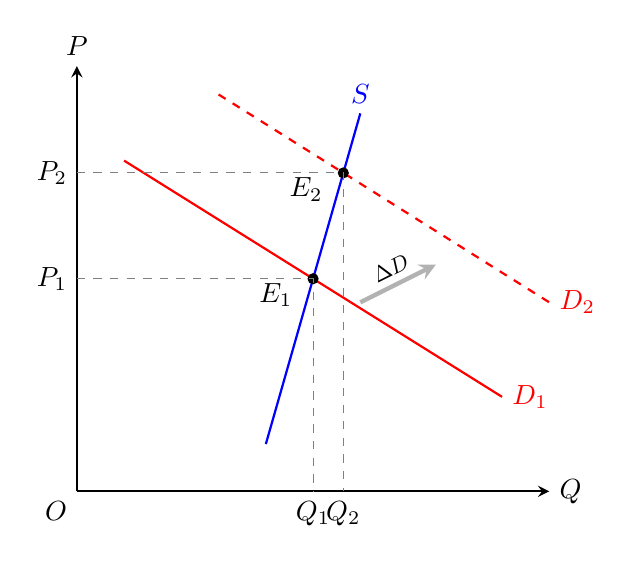
\begin{tikzpicture}[scale=1.2, >=stealth]
				% 坐标轴
				\draw[->, thick] (0,0) -- (5,0) node[right] {$Q$};
				\draw[->, thick] (0,0) -- (0,4.5) node[above] {$P$};
				\node[below left] at (0,0) {$O$};
				
				\draw[thick, blue] (2,0.5) -- (3,4) node[above] {$S$};
				
				% 初始需求曲线 D1
				\draw[thick, red] (0.5,3.5) -- (4.5,1) node[right] {$D_1$};
				
				% 新需求曲线 D2
				\draw[thick, red, dashed] (1.5,4.2) -- (5,2) node[right] {$D_2$};
				
				% 均衡点标注 
				\filldraw (2.5,2.25) circle (1.5pt) node[left, xshift=-4pt,yshift=-6pt] {$E_1$};
				\filldraw (2.82,3.37) circle (1.5pt) node[left, xshift=-4pt,yshift=-6pt] {$E_2$};
				
				% 价格与数量辅助线
				\draw[dashed, gray] (0,2.25) node[left, black] {$P_1$} -- (2.5,2.25) -- (2.5,0) node[below, black] {$Q_1$};
				\draw[dashed, gray] (0,3.37) node[left, black] {$P_2$} -- (2.82,3.37) -- (2.82,0) node[below, black] {$Q_2$};
				
				% 需求移动箭头
				\draw[->, ultra thick, gray!60] (3.0,2.0) -- (3.8,2.4) node[midway, sloped, above, scale=0.8, black] {$\Delta D$};
			\end{tikzpicture}
		\end{center}
		
		在短期内，由于生产商的产能和库存难以迅速调整，供给曲线通常表现得非常陡峭（即缺乏弹性）。当需求曲线从 $D_1$ 右移至 $D_2$ 时，在原均衡价格 $P_1$ 水平上会出现显著的短缺。
		
		这种短缺压力会促使未买到商品的消费者竞相出价，同时零售商也会随之提高售价。随着价格的攀升，一部分需求被抑制，最终在更高的价格水平 $P_2$ 上重新实现供需平衡。
		
			\item \textbf{运用供给曲线和需求曲线说明以下各事件会怎样影响黄油的价格以及黄油的销售量、购买量：}
			\begin{enumerate}[label=(\alph*), leftmargin=2em]
				\item \textbf{人造黄油价格上升；}
				\item \textbf{牛奶价格上升；}
				\item \textbf{平均收入水平下降。}
			\end{enumerate}
			
			\textbf{答：}
			分析这些事件对均衡价格（$P$）和均衡数量（$Q$）的影响，需识别受冲击的是需求侧还是供给侧。
			
				(a)人造黄油与黄油互为替代品。人造黄油价格上升，消费者会转而消费黄油，导致黄油需求增加，价格与销量同步上升。
				
				(b)牛奶是生产黄油的核心原材料。牛奶价格上涨抬高了生产成本，导致供给减少，表现为供给曲线向左上方移动。
				
				(c)黄油通常被视为正常商品。收入水平下降导致消费者购买力减弱，需求曲线向左下方移动。
			
			\item \textbf{如果玉米片的价格上升3\%致使其需求量下降6\%，那么玉米片的需求价格弹性是多少？}
			
			\textbf{答：}
			需求价格弹性的核心定义式如下：
				$$ E_d = \frac{\Delta Q / Q}{\Delta P /P} $$
			
			已知需求量变动 $-6\%$，价格变动 $3\%$。代入公式计算得：
				$$ E_d = \frac{-6\%}{3\%} = -2 $$
			由于 $|E_d| = 2 > 1$，说明玉米片的需求是富有弹性的。

			\item \textbf{试解释供给曲线的移动和沿着供给曲线的移动之间的区别。}
			
			\textbf{答：}
			这两者的根本区别在于引发变动的因素不同。
			
			沿着供给曲线的移动由商品自身价格变动引起。供给曲线整体位置保持不变，仅均衡点在原有供给曲线上上下滑动，仅改变供给数量，不改变供给整体水平。
			
			供给曲线的移动由生产成本、技术、相关品价格、预期等非价格因素变动引起。商品每一价格对应的供给数量整体发生改变，表现为整条供给曲线向左或向右平移，代表供给整体增加或减少。
			
			图形直观对比示意见下：
			
		\begin{center}
			\begin{tikzpicture}[scale=1.1, >=stealth]
				% --- 左图：供给曲线整体移动 ---
				\draw[->, thick] (0,0) -- (3.5,0) node[right] {$Q$};
				\draw[->, thick] (0,0) -- (0,3.5) node[above] {$P$};
				\draw[thick] (0.8,0.5) -- (3.2,3.2) node[above] {$S_1$};
				\draw[thick, dashed, blue] (0.2,0.5) -- (2.6,3.2) node[above] {$S_2$};
				
				\draw[->, blue, thick] (1.6,1.5) -- (1.2,1.5);
				\node[below] at (1.7, -0.4) {\textbf{(a) 曲线的移动 (线变动)}};
				
				% --- 右图：沿供给曲线点移动 ---
				\begin{scope}[xshift=5.5cm]
					\draw[->, thick] (0,0) -- (3.5,0) node[right] {$Q$};
					\draw[->, thick] (0,0) -- (0,3.5) node[above] {$P$};
					\draw[thick] (0.8,0.5) -- (3.2,3.2) node[above] {$S$};

					\coordinate (A) at (1.5,1.29);
					\coordinate (B) at (2.5,2.41);
					
					\fill (A) circle (1.5pt) node[below right] {$A$};
					\fill (B) circle (1.5pt) node[below right] {$B$};

					\draw[->, red, thick, bend right=25, shorten <=3pt, shorten >=3pt] (A) to (B);
					
					\node[below] at (1.7, -0.4) {\textbf{(b) 沿着曲线移动 (点变动)}};
				\end{scope}
			\end{tikzpicture}
		\end{center}
		\item \textbf{试解释为什么许多商品的长期需求弹性要大于短期需求弹性。}
		
		\textbf{答：}
		商品长期需求弹性大于短期需求弹性，核心源于消费者调整行为的时间差异。短期中，消费习惯与消费结构难以快速改变，替代品选择有限，面对价格波动，需求量仅能小幅调整，需求弹性较小。长期条件下，消费者可充分调整消费偏好、更换替代商品、优化消费方案，对价格变化做出充分反应。相同价格变动幅度下，长期需求量的调整幅度更大，因此长期需求弹性更高。
		
		\newpage
		\item \textbf{为什么长期需求弹性与短期需求弹性会有不同？考虑两种商品：纸巾和电视机。哪一种是耐用品？你觉得纸巾的短期需求价格弹性大，还是长期需求价格弹性大？为什么？电视机的需求价格弹性又是怎样的？}
		
		\textbf{答：}
		长期需求弹性与短期需求弹性存在差异，核心在于消费者调整行为所需的时间。电视机属于耐用品，纸巾为日常非耐用消耗品。二者的弹性特征对比如下表所示：
		
		\begin{center}
			\begin{tabularx}{\textwidth}{>{\centering\arraybackslash}X >{\centering\arraybackslash}X >{\centering\arraybackslash}X}
				\toprule
				\textbf{商品类别} & \textbf{短期需求价格弹性} & \textbf{长期需求价格弹性} \\
				\midrule
				纸巾（非耐用消耗品） & 较小 & 较大 \\
				电视机（耐用品） & 较大 & 较小 \\
				\bottomrule
			\end{tabularx}
		\end{center}

		\textbf{纸巾（非耐用消耗品）：长期需求价格弹性更大。}在短期内，人们的生活习惯和消费结构可能很难改变，对价格变化并没有太多反应；但是在长期中，人们会有充足的时间寻找替代品（如改用抹布)或者是改变自己的生活习惯，因此在这个过程中，需求量对于价格的反映就会变得更加灵敏一些。
		
		\textbf{电视机（耐用品）：短期需求价格弹性更大。}因为电视机购买往往具有一定延迟性。当电视机的价格短期上涨时，人们完全可以选择继续使用旧电视而不换新，其短期需求量会剧烈下降（弹性大）；但是在长期里，旧电视将最终报废，即便面临高昂的成本也必须要购买，所以从长期来看，它只有相对较小的需求量（弹性小）。
		
		\item \textbf{以下陈述是否正确？请解释。\\
			a. 需求的价格弹性等于需求曲线的斜率。\\
			b. 交叉价格弹性总是为正。\\
			c. 公寓的短期供给弹性要低于其长期供给弹性。}
		
		\textbf{答：}
		
		\textbf{a. 错误。}
		
		需求价格弹性核心公式如下：

			$$E_d = \frac{\Delta Q/Q}{\Delta P/P} = \frac{\Delta Q}{\Delta P} \cdot \frac{P}{Q}$$

		
		需求曲线斜率为 $\frac{\Delta P}{\Delta Q}$，二者并不等同。弹性除受斜率影响外，还受 $P/Q$ 比值影响。线性需求曲线上斜率恒定，但不同点位的 $P$ 和 $Q$ 不同，因此每一点需求价格弹性均不相等。
		
		\textbf{b. 错误。}
		
		交叉价格弹性核心公式如下：

			$$E_{XY} = \frac{\Delta Q_X/Q_X}{\Delta P_Y/P_Y}$$

		
		交叉价格弹性可正、可负，并非恒为正数。具体分类及其经济学含义如下表所示：
		
		\begin{center}
			\renewcommand{\tabularxcolumn}[1]{m{#1}}
			\begin{tabularx}{\textwidth}{>{\centering\arraybackslash}X >{\centering\arraybackslash}X >{\centering\arraybackslash}X}
				\toprule
				\textbf{商品关系} & \textbf{交叉价格弹性符号} & \textbf{特征描述} \\
				\midrule
				替代品 & 正数（$E_{XY} > 0$） & 一种商品价格上升，导致另一种商品需求量增加 \\
				互补品 & 负数（$E_{XY} < 0$） & 一种商品价格上升，导致另一种商品需求量减少 \\
				\bottomrule
			\end{tabularx}
		\end{center}

		\textbf{c. 正确。}
		
		公寓属于长期建设的不动产，短期房屋数量、楼栋规模难以调整，供给刚性强，短期供给弹性小；长期可通过新建、改造、盘活房源等方式调整供给数量，供给调整空间更大，因此长期供给弹性更高。
		
		\item \textbf{政府对牛肉、鸡肉实施低于市场出清水平的价格管制，分析其对市场及替代品的影响。}
		
		\textbf{答：}
		
		市场短缺状态的形成机制如下：
		\begin{tcolorbox}[colback=white, colframe=black!10, sharp corners, boxrule=0.5pt]
			$$\text{当 } P_{\text{限价}} < P_{\text{均衡}} \text{ 时，} Q_D > Q_S \implies \text{市场出现短缺}$$
		\end{tcolorbox}
		
		政府对牛肉、鸡肉实施低于市场出清水平的价格管制，属于最高限价政策。在管制低价下，生产者利润被压缩，供给量减少；消费者购买成本下降，需求量增加。由此形成 $Q_D > Q_S$ 的市场状态，出现商品短缺。短缺的规模由需求价格弹性与供给价格弹性共同决定：供需弹性越小，供需数量调整幅度越有限，短缺问题越突出。
		
		牛肉、鸡肉与猪肉互为替代品，前者因限价出现供给短缺时，消费者会转向消费猪肉，推动猪肉需求曲线右移，最终导致猪肉均衡价格上升。长期过低的行政限价，还会引发排队抢购、黑市交易、非价格配给等市场乱象，降低资源配置效率。
		
		\begin{center}
			\begin{tikzpicture}[scale=1.2, >=stealth]
				% --- 1. 定义坐标点  ---
				\coordinate (O) at (0,0);
				\coordinate (E) at (2.75, 2.75); 
				\coordinate (P_max_line) at (0, 1.75); 
				\coordinate (Qs_point) at (1.75, 1.75); 
				\coordinate (Qd_point) at (3.75, 1.75); 
				
				% --- 2. 绘制坐标轴 ---
				\draw[->, thick] (O) -- (6,0) node[right] {$Q$};
				\draw[->, thick] (O) -- (0,5) node[above] {$P$};
				\node[below left] at (O) {$O$};
				
				% --- 3. 绘制供给 S 与需求 D 曲线 ---
				\draw[thick] (0.8, 0.8) -- (4.5, 4.5) node[right] {$S$};
				\draw[thick] (0.8, 4.7) -- (4.8, 0.7) node[right] {$D$};
				
				% --- 4. 标注原均衡价格 P0 ---
				\draw[dashed, gray] (0, 2.75) node[left, black] {$P_0$} -- (E);
				\filldraw[black] (E) circle (1.5pt) node[above=2pt] {$E$};
				
				% --- 5. 绘制最高限价 (Price Ceiling) ---
				\draw[thick, blue] (0, 1.75) node[left] {$P_{\text{限价}}$} -- (5, 1.75);
				
				% 标注交点并投影到横轴
				\filldraw (Qs_point) circle (1.5pt);
				\filldraw (Qd_point) circle (1.5pt);
				
				\draw[dashed] (Qs_point) -- (1.75, 0) node[below] {$Q_s$};
				\draw[dashed] (Qd_point) -- (3.75, 0) node[below] {$Q_d$};
				
				% --- 6. 标注短缺区间 (Shortage) ---
				% 将箭头放在限价线上方一点，避免遮挡Q轴投影
				\draw[<->, red, thick] (1.75, 1.2) -- (3.75, 1.2) 
				node[midway, above, black, font=\small] {短缺};
				
			\end{tikzpicture}
		\end{center}
		\newpage
		\item \textbf{假设初始租房市场的市场出清租金为每月 700 美元。随着城市发展，租房需求增加，无管制的自由市场中新均衡租金上升至每月 900 美元。如果政府实施租金管制，设定最高租金限制为 700 美元。请分析：（1）租金变化与市场均衡情况；（2）租金管制是否对所有学生有利？}
		
		\textbf{答：}
		
		(1)租金变化与市场均衡分析
		
		初始租房市场自发均衡，市场出清租金为每月 700 美元。随城市发展，租房需求增加，需求曲线向右平移，在无管制的自由市场中，新均衡租金上升至每月 900 美元。
		
		政府实施租金管制，设定最高租金限制为 700 美元，该价格低于新市场均衡价格，属于限制性价格上限。短期住房供给弹性极低、供给数量近似固定；管制低价刺激租房需求进一步扩张，供给意愿小幅下降，市场出现供不应求与房源短缺。
		
		租金变动总结：自由市场下租金先由 700 美元上涨至 900 美元，管制政策将价格强行锁定在 700 美元，整体表现为先上升、后被管制压低。
		
		\begin{center}
			\begin{tikzpicture}[scale=0.8, >=stealth, thick, 
				dot/.style={circle, fill=black, inner sep=1pt}, every node/.style={scale=0.85}]
				
				% --- 1. 坐标轴 ---
				\draw[->] (0,0) coordinate(O) -- (7.5,0) node[right] {$Q$ \small (住房数量)};
				\draw[->] (0,0) -- (0,5.5) node[above] {$P$ \small (月租金/美元)};
				\node[below left] at (O) {$O$};
				
				% --- 2. 坐标点定义 ---
				\coordinate (E0) at (3, 2.5);     % 初始均衡点
				\coordinate (E1) at (3.5, 3.5);   % 新均衡点
				\coordinate (Qd_p) at (4.5, 2.5); % 限价下的新需求量点
				
				% --- 3. 绘制供需曲线 ---
				% 供给曲线 S
				\draw[black, ultra thick] (2, 0.5) -- (4.25, 5) node[right] {$S$};
				% 初始需求 D0
				\draw[black, thick] (1, 4.5) -- (5, 0.5) node[right] {$D_0$};
				% 新需求 D1
				\draw[blue, thick, dashed] (2.5, 4.5) -- (6.5, 0.5) node[right] {$D_1$};
				
				% --- 4. 需求曲线移动箭头 ---
				% 在上方空白处增加指示箭头，颜色与 D1 一致
				\draw[->, blue!80!black, thick] (1.9, 3.8) -- (3.0, 3.8) node[midway, above, font=\small] {};
				
				% --- 5. 价格上限线 (红色) ---
				\draw[red, ultra thick] (0, 2.5) -- (6.8, 2.5) 
				node[pos=0.1, above, text=red, font=\small\bfseries] {价格上限};
				
				% --- 6. 绘制垂直投影虚线 ---
				% 使用正交语法保证垂直
				\draw[dashed, gray] (E0) -- (E0 |- O) node[below, black] {$Q_0$};
				\draw[dashed, gray] (E1) -- (E1 |- O) node[below, black] {$Q_1$};
				\draw[dashed, gray] (Qd_p) -- (Qd_p |- O) node[below, black] {$Q_d$};
				
				% 仅保留 P1 的纵轴投影，移除 P0 投影
				\draw[dashed, gray] (E1) -- (O |- E1) node[left, black] {$P_1=900$};
				% 轴上的价格刻度（不需要虚线引导）
				\node[left] at (0, 2.5) {$P_0=700$};
				
				% --- 7. 标注交点 (调整位置防止遮挡) ---
				\node[dot] at (E0) {};
				\node[below left, xshift=-2pt] at (E0) {$E_0$}; % 移至左下方，避开 S 线
				
				\node[dot] at (E1) {};
				\node[right, xshift=3pt] at (E1) {$E_1$}; % 移至右侧，避开 D1 线
				
				\node[dot] at (Qd_p) {};
				
				% --- 8. 短缺标注 ---
				\draw[<->, red, very thick] ([yshift=-12pt]E0) -- ([yshift=-12pt]Qd_p) 
				node[midway, fill=white, inner sep=2pt, font=\small\bfseries] {短缺};
				
			\end{tikzpicture}
		\end{center}
		
		(2)租金管制是否对所有学生有利？
		
		否，政策带来福利分化，并非全体学生受益。对于已租房的在校学生，若无管制，房租将上涨至 900 美元/月；价格上限锁定租金为 700 美元，直接降低居住成本，福利改善。而对于尚未租房的潜在租客，短期住房供给刚性、房源总量有限。管制低价催生超额需求，房源竞争加剧，大量学生难以租到住房；同时易出现居住条件下降、隐性收费等问题，该群体利益受损。
		
		\item \textbf{某大学官员宣称，学费上涨并未减少申请入学的人数，反而由于该校声誉和教育质量的提升，申请人数显著增加。他据此认为该校的入学需求是完全无弹性的。请评述该官员的观点。}
		
		\textbf{答：}
		该大学官员的观点是错的。其核心在于混淆了“需求量的变动”与“需求的变动”，未能遵循经济学分析中“其他条件不变”的准则。
		
		该官员认为学费上涨没有减少申请人数，证明需求完全无弹性（即需求曲线是垂直的）。然而，经济学原理告诉我们，在其他条件不变的前提下，学费作为价格，其上涨必然导致需求量下降。
		
		现实中申请人数不降反升，并不是因为需求没有弹性，而是因为需求曲线发生了整体右移。该官员提到的“声誉提升”和“质量改善”，以及居民收入增加等因素，都是影响需求的非价格变量。这些因素的正面冲击足以抵消学费上涨带来的需求量缩减，导致最终观察到的均衡数量增加。
		
		市场变动示意图如下：
		\begin{center}
			\begin{tikzpicture}[scale=0.8, >=stealth, thick, 
				dot/.style={circle, fill=black, inner sep=1pt}, every node/.style={scale=0.85}]
				
				% --- 1. 坐标轴 ---
				\draw[->] (0,0) coordinate(O) -- (7,0) node[right] {$Q$ \small (申请人数)};
				\draw[->] (0,0) -- (0,5.5) node[above] {$P$ \small (学费)};
				\node[below left] at (O) {$O$};
				
				% --- 2. 坐标点 (根据直线方程求解) ---
				\coordinate (E0) at (3, 3);
				\coordinate (Qa) at (1.933, 3.8); 
				\coordinate (E1) at (3.433, 3.8); 
				
				% --- 3. 需求曲线 ---
				% 原需求 D0 (黑色)
				\draw[black, thick] (1, 4.5) -- (5, 1.5) node[below right] {$D_0$};
				% 新需求 D1 (蓝色虚线，代表右移)
				\draw[blue, thick, dashed] (2.5, 4.5) -- (6.5, 1.5) node[below right] {$D_1$};
				% 官员脑补的垂直需求曲线 (灰色点线)
				\draw[gray, dotted, ultra thick] (3, 0.5) -- (3, 5) node[above, font=\small, text=gray] {官员假设的 $D$};
				
				% --- 4. 均衡点与投影 ---
				% 初始均衡 E0
				\draw[dashed, gray] (E0) -- (0, 3) node[left, black] {$P_0$};
				\draw[dashed, gray] (E0) -- (3, 0) node[below, black] {$Q_0$};
				\node[dot] at (E0) {};
				\node[below left] at (E0) {$E_0$};
				
				% 涨价后的横向价格线 P1，贯穿 Qa 和 E1
				\draw[dashed, gray] (0, 3.8) node[left, black] {$P_1$} -- (E1);
				
				% 沿 D0 移动的 Qa 点 (价格效应终点)
				\draw[dashed, gray] (Qa) -- (Qa |- O) node[below, black] {$Q'$};
				\node[dot] at (Qa) {};
				
				% 最终新均衡 E1
				\draw[dashed, gray] (E1) -- (E1 |- O) node[below, black] {$Q_1$};
				\node[dot] at (E1) {};
				\node[above right] at (E1) {$E_1$};
				
				% --- 5. 动态标注 ---
				% 需求移动箭头
				\draw[->, blue!80!black, ultra thick] (3.8, 2.4) -- (5.2, 2.4) ;
				
				% 价格上涨引起的点动箭头
				\draw[->, red, very thick, bend right=15, shorten <=3pt, shorten >=3pt] (E0) to (Qa);
				
			\end{tikzpicture}
		\end{center}
		
		结论：该官员将“需求的变动”（曲线右移）错误地解读为“需求完全无弹性”。如果该校保持学费不变，申请人数本应增加更多（增加到 $D_1$ 在 $P_0$ 对应的水平）。因此，不能依据学费和人数同步增长的事实来断定需求缺乏弹性。

		\item \textbf{假设某种商品的需求曲线为 $Q=10-2P+P_S$，其中，$P$ 是该商品的价格，$P_S$ 是某种替代品的价格。已知该替代品的价格是 $2.00$ 美元。a. 如果 $P=1.00$ 美元，需求的价格弹性等于多少？交叉价格弹性又等于多少？b. 如果该商品的价格 $P$ 上升至 $2.00$ 美元，那么现在需求的价格弹性又是多少？交叉价格弹性呢？}
		
		\textbf{答：}
		将已知替代品价格 $P_S = 2.00$ 代入需求函数，可得化简后的商品需求方程：
		$$Q = 12 - 2P$$
		根据点弹性定义，建立需求价格弹性与交叉价格弹性的核心计算公式：

			$$
			\begin{aligned}
				E_d &= \frac{\partial Q}{\partial P} \cdot \frac{P}{Q}\\
				E_{xy} &= \frac{\partial Q}{\partial P_S} \cdot \frac{P_S}{Q}
			\end{aligned}
			$$

		
		a.当商品价格 $P = 1.00$ 时，对应的市场需求量为 $Q = 10$。代入核心公式计算可得：
		$$
		\begin{aligned}
			E_d &= -2 \times \frac{1.00}{10} = -0.2 \\
			E_{xy} &= \frac{2.00}{10} = 0.2
		\end{aligned}
		$$
		此时 $|E_d| < 1$，表明该价格水平下需求缺乏弹性；$E_{xy} > 0$ 则验证了两种商品互为替代品的经济关系。
		
		b.当商品价格上升至 $P = 2.00$ 时，需求量缩减为 $Q = 8$。重新测算两类弹性：
		$$
		\begin{aligned}
			E_d &= -2 \times \frac{2.00}{8} = -0.5 \\
			E_{xy} &= \frac{2.00}{8} = 0.25
		\end{aligned}
		$$
		计算结果表明，随着价格沿线性需求曲线向上攀升，需求价格弹性的绝对值逐渐增大，消费者对价格变动的敏感度提升。

		\item \textbf{已知铜市场的初始需求曲线为 $Q_d = 27 - 3P$，初始供给曲线为 $Q_s = -9 + 9P$。若生产成本下降导致供给曲线向右移动 40\%，请推导新的供给曲线，计算新的市场均衡，并结合图形分析市场的具体变动。}
		
		\textbf{答：}
		在原有市场结构下，若生产成本发生下降，生产者在任何给定的价格水平下都有能力且愿意提供更多的产品。根据题意，供给曲线整体向右移动 40\%，等价于新供给量等于原供给量的 1.4 倍。由此可推导出新的供给函数方程：
			$$Q'_s = 1.4(-9 + 9P) = -12.6 + 12.6P$$
		
		市场出清原则要求新的总供给量必须等于总需求量。令原需求曲线 $Q_d$ 与新供给曲线 $Q'_s$ 相等，构建均衡等式进行求解：
		$$
		\begin{aligned}
			Q_d &= Q'_s \\
			P &\approx 2.54 \text{ 美元/磅}
		\end{aligned}
		$$
		将计算得到的新均衡价格代回原需求方程，可求得此时的新均衡交易量为 $Q \approx 27 - 3(2.54) = 19.38 \text{ 百万公吨/年}$。

		\begin{center}
			\begin{tikzpicture}[x=0.1875cm, y=0.9cm, >=stealth, every node/.style={scale=0.85}]
				% 坐标轴
				\draw[->, thick] (0,0) -- (28,0) node[right] {$Q \text{ (百万公吨/年)}$};
				\draw[->, thick] (0,0) -- (0,5.5) node[above] {$P \text{ (美元/磅)}$};
				
				% 原需求曲线 D: P = 9 - Q/3 
				\draw[thick, name path=demand] (10, 5.67) -- (26, 0.33) node[below right] {$D$};
				
				% 原供给曲线 S: P = 1 + Q/9 
				\draw[thick, name path=supply0] (4.5, 1.5) -- (26, 3.89) node[above right] {$S$};
				
				% 新供给曲线 S': P = 1 + Q/12.6 
				\draw[thick, blue, dashed, name path=supply1] (6.3, 1.5) -- (26, 3.06) node[right] {$S'$};
				
				% 初始均衡点 E
				\coordinate (E0) at (18, 3);
				\fill (E0) circle (2pt) node[above=4pt, fill=white, inner sep=1pt] {$E$};
				\draw[dashed] (E0) -- (E0 |- 0,0) node[below, fill=white, inner sep=1pt] {$18$};
				\draw[dashed] (E0) -- (0,0 |- E0) node[left] {$3.00$};
				
				% 新均衡点 E'
				\coordinate (E1) at (19.38, 2.54);
				\fill (E1) circle (2pt) node[below left=2pt, fill=white, inner sep=1pt] {$E'$};
				\draw[dashed] (E1) -- (E1 |- 0,0) node[below, fill=white, inner sep=1pt] {$19.38$};
				\draw[dashed] (E1) -- (0,0 |- E1) node[left] {$2.54$};
				
				\coordinate (A) at (9, 2);
				\coordinate (B) at (12, 2);
				\draw[->, thick, blue, shorten <=3pt, shorten >=3pt] (A) -- (B);
			\end{tikzpicture}
		\end{center}

		\item \textbf{假设天然气的需求是完全无弹性的，那么对天然气的价格控制可能会导致什么样的后果？}
		
		\textbf{答：}
		如果天然气的需求完全没有弹性，无论价格怎么变，消费者购买的数量固定。在坐标轴里，需求曲线就是一条垂直的直线。
		
		这时，如果政府干预价格，市场失衡的程度主要取决于供给方的反应。限价或保价政策，会引向截然不同的局面。供应越灵活，市场缺口（无论是短缺还是过剩）就拉得越大。以下是两种政策下的市场变动分析：
		\begin{center}
			\begin{tikzpicture}[scale=1.1, >=stealth]
				% ---------- 左图：最低限价（供给过剩） ----------
				\begin{scope}[shift={(0,0)}]
					% 坐标轴
					\draw[->, thick] (0,0) -- (4.5,0) node[right] {$Q$};
					\draw[->, thick] (0,0) -- (0,4.5) node[above] {$P$};
					
					% 完全无弹性需求曲线 D（垂直，基准线黑）
					\draw[thick, name path=demand1] (2,0) -- (2,4.3) node[above] {$D$};
					
					% 供给曲线 S（基准线黑）
					\draw[thick, name path=supply1] (0.5,0.5) -- (3.5,3.5) node[above right] {$S$};
					
					% 均衡点 E
					\coordinate (E1) at (2,2);
					\fill (E1) circle (1.5pt) node[above left] {$E$};
					\draw[dashed] (E1) -- (E1 |- 0,0) node[below] {$Q^*$};
					\draw[dashed] (E1) -- (0,0 |- E1) node[left] {$P^*$};
					
					% 最低限价 Pmin (政策限制线，红粗)
					\draw[very thick, red] (0,3) node[left] {$P_{\min}$} -- (4,3);
					
					% 供给点与需求点投影
					\coordinate (S1) at (3,3);
					\coordinate (D1) at (2,3);
					\fill (S1) circle (1.5pt);
					\fill (D1) circle (1.5pt);
					\draw[dashed] (S1) -- (S1 |- 0,0) node[below] {$Q_s$};
					
					% 标识失衡区间
					\draw[<->, thick, shorten <=2pt, shorten >=2pt] (2, 0.5) -- (3, 0.5) node[midway, below] {\small 过剩};
				\end{scope}
				
				% ---------- 右图：最高限价（供给短缺） ----------
				\begin{scope}[shift={(6,0)}]
					% 坐标轴
					\draw[->, thick] (0,0) -- (4.5,0) node[right] {$Q$};
					\draw[->, thick] (0,0) -- (0,4.5) node[above] {$P$};
					
					% 完全无弹性需求曲线 D（垂直，基准线黑）
					\draw[thick, name path=demand2] (2,0) -- (2,4.3) node[above] {$D$};
					
					% 供给曲线 S（基准线黑）
					\draw[thick, name path=supply2] (0.5,0.5) -- (3.5,3.5) node[above right] {$S$};
					
					% 均衡点 E
					\coordinate (E2) at (2,2);
					\fill (E2) circle (1.5pt) node[above left] {$E$};
					\draw[dashed] (E2) -- (E2 |- 0,0) node[below] {$Q^*$};
					\draw[dashed] (E2) -- (0,0 |- E2) node[left] {$P^*$};
					
					% 最高限价 P_max (政策限制线，红粗)
					\draw[very thick, red] (0,1) node[left] {$P_{\max}$} -- (4,1);
					
					% 供给点与需求点投影
					\coordinate (S2) at (1,1);
					\coordinate (D2) at (2,1);
					\fill (S2) circle (1.5pt);
					\fill (D2) circle (1.5pt);
					\draw[dashed] (S2) -- (S2 |- 0,0) node[below] {$Q_s$};
					
					% 标识失衡区间
					\draw[<->, thick, shorten <=2pt, shorten >=2pt] (1, 0.5) -- (2, 0.5) node[midway, below] {\small 短缺};
				\end{scope}
			\end{tikzpicture}
		\end{center}
	\end{enumerate}
	\newpage
	\section{练习题}
		\begin{enumerate}[label=\textbf{\arabic*.}, leftmargin=*]
			\item \textbf{假设某种商品的需求曲线是 $Q=300-2P+4I$，其中 $I$ 是以千美元计量的收入。供给曲线是 $Q=3P-50$。请分别求解当 $I=25$ 和 $I=50$ 时的市场出清价格与数量，并画图说明。}
			
			\textbf{答：}
			当 $I=25$ 时，代入需求函数可得当期需求曲线为 $Q_d = 400 - 2P$。根据市场出清条件 $Q_d = Q_s$，直接列式：
			$$ 400 - 2P = 3P - 50 \implies P = 90,\ Q = 220 $$
			当 $I=50$ 时，需求曲线变动为 $Q_d = 500 - 2P$。同理：
			$$ 500 - 2P = 3P - 50 \implies P = 110,\ Q = 280 $$
			由此可见，收入增加使得需求曲线整体右移，带动市场均衡价格与数量双双上升。其市场供需变动图形如下：
			\begin{center}
				\begin{tikzpicture}[x=0.0225cm, y=0.0375cm, >=stealth, every node/.style={scale=0.8}]
					% 坐标轴
					\draw[->, thick] (0,0) -- (350,0) node[right] {$Q$};
					\draw[->, thick] (0,0) -- (0,150) node[above] {$P$};
					
					% 供给与需求曲线
					\draw[thick, name path=S] (50, 33.33) -- (320, 123.33) node[above right] {$S$};
					\draw[thick, name path=D1] (100, 150) -- (300, 50) node[below right] {$D_1 (I=25)$};
					\draw[thick, blue, dashed, name path=D2] (160, 170) -- (320, 90) node[right] {$D_2 (I=50)$};
					
					% 均衡点 E1
					\coordinate (E1) at (220, 90);
					\fill (E1) circle (1.5pt) node[below left=2pt, fill=white, inner sep=1pt] {$E_1$};
					\draw[dashed] (E1) -- (E1 |- 0,0) node[below] {$220$};
					\draw[dashed] (E1) -- (0,0 |- E1) node[left] {$90$};
					
					% 均衡点 E2
					\coordinate (E2) at (280, 110);
					\fill (E2) circle (1.5pt) node[above right=2pt, fill=white, inner sep=1pt] {$E_2$};
					\draw[dashed] (E2) -- (E2 |- 0,0) node[below] {$280$};
					\draw[dashed] (E2) -- (0,0 |- E2) node[left] {$110$};
					
					% 需求右移指示箭头
					\draw[->, thick, blue, shorten <=4pt, shorten >=4pt] (160, 120) -- (250, 120) node[midway, below, fill=white, inner sep=1pt] {\small \text{需求增加}};
				\end{tikzpicture}
			\end{center}
			
			
			\item \textbf{考虑一个竞争性市场，在不同价格下，需求量和供给量如下表所示。请计算价格在 80 美元至 100 美元区间的需求/供给价格弹性，指出均衡状态，并分析 80 美元最高限价的政策影响。}
			\begin{center}
				\begin{tabularx}{\textwidth}{>{\centering\arraybackslash}X >{\centering\arraybackslash}X >{\centering\arraybackslash}X}
					\toprule
					\textbf{价格（美元）} & \textbf{需求量（百万）} & \textbf{供给量（百万）} \\
					\midrule
					60 & 22 & 14 \\
					80 & 20 & 16 \\
					100 & 18 & 18 \\
					120 & 16 & 20 \\
					\bottomrule
				\end{tabularx}
			\end{center}
			
			\textbf{答：}
			首先，计算需求与供给价格弹性。在 80 至 100 美元区间，需求曲线斜率为$-0.1$，供给曲线斜率为 $0.1$。用点弹性核心公式进行计算：
				$$ E = \frac{\Delta Q}{\Delta P} \cdot \frac{P}{Q} $$
			将对应数据代入公式，直接求解得出：
			$$
			\begin{aligned}
				\text{当 } P=80 \text{ 时：} & E_d = -0.1 \times \frac{80}{20} = -0.4, \quad E_s = 0.1 \times \frac{80}{16} = 0.5 \\
				\text{当 } P=100 \text{ 时：} & E_d = -0.1 \times \frac{100}{18} \approx -0.56, \quad E_s = 0.1 \times \frac{100}{18} \approx 0.56
			\end{aligned}
			$$
			
			由表格数据直观可知，当价格 $P=100$ 美元时，市场需求量等于供给量，即均衡价格 $P^* = 100$，均衡数量 $Q^* = 18$。
			
			若政府设定80美元的最高限价，该价格低于均衡价格，属于有效价格干预。此时市场需求量上升至20，而供给量降低至16，直接列式计算短缺缺口：
			$$ \text{短缺量} = Q_d - Q_s = 20 - 16 = 4 $$
			\begin{center}
				\begin{tikzpicture}[x=0.3cm, y=0.0375cm, >=stealth, every node/.style={scale=0.8}]
					% 坐标轴
					\draw[->, thick] (0,0) -- (26,0) node[right] {$Q \text{ (百万)}$};
					\draw[->, thick] (0,0) -- (0,150) node[above] {$P \text{ (美元)}$};
					
					% 需求与供给曲线
					\draw[thick, name path=demand] (14, 140) -- (24, 40) node[below right] {$D$};
					\draw[thick, name path=supply] (12, 40) -- (22, 140) node[above right] {$S$};
					
					% 均衡点 E
					\coordinate (E) at (18, 100);
					\fill (E) circle (1.5pt) node[above=4pt] {$E$};
					\draw[dashed] (E) -- (E |- 0,0) node[below] {$18$};
					\draw[dashed] (E) -- (0,0 |- E) node[left] {$100$};
					
					% 最高限价 (政策线，红粗)
					\draw[very thick, red] (0, 80) node[left] {$80$} -- (25, 80) node[right] {$P_{\max}$};
					
					% 短缺投影与标识
					\coordinate (Qs) at (16, 80);
					\coordinate (Qd) at (20, 80);
					\fill (Qs) circle (1.5pt);
					\fill (Qd) circle (1.5pt);
					\draw[dashed] (Qs) -- (Qs |- 0,0) node[below] {$16$};
					\draw[dashed] (Qd) -- (Qd |- 0,0) node[below] {$20$};
					
					% 调整短缺标识的比例
					\draw[<->, thick, shorten <=2pt, shorten >=2pt] (16, 20) -- (20, 20) node[midway, below, fill=white, inner sep=1pt] {\small $\text{短缺}$};
				\end{tikzpicture}
			\end{center}
			
			\item \textbf{在 1998 年，美国对小麦的需求函数为 $Q_d = 3244 - 283P$，本国供给函数为 $Q_s = 1944 + 207P$。假设巴西和印度尼西亚开放市场后，美国小麦的需求增加了 200 百万蒲式耳。求新的完全竞争均衡价格与产量。}
			
			\textbf{答：}
			国际市场的开放导致美国小麦需求增加。这表现为在任何给定的价格水平下，需求量均增加 200 百万蒲式耳。因此，新的市场需求函数方程变为：
			$$Q'_d = (3244 - 283P) + 200 = 3444 - 283P$$
			
			在供给曲线 $Q_s = 1944 + 207P$ 保持不变的情况下，令新需求等于供给 $Q'_d = Q_s$，直接列式计算新的市场出清状态：
			$$3444 - 283P = 1944 + 207P \implies P \approx 3.06 \text{ 美元},\ Q \approx 2577 \text{ 百万蒲式耳}$$
			
			外部市场开放带来的需求扩张直接拉高了小麦的市场价格，并同时推高了总产出规模。

			\item \textbf{一种植物纤维在竞争性的世界市场上进行贸易，世界市场价格为9美元/磅。在该价格下，美国可以得到无限多的进口商品。在不同的价格水平下，美国国内市场的供给和需求如下表所示：}
			
			\begin{center}
				\begin{tabularx}{\textwidth}{>{\centering\arraybackslash}X >{\centering\arraybackslash}X >{\centering\arraybackslash}X}
					\toprule
					\textbf{价格} & \textbf{美国的供给（百万磅）} & \textbf{美国的需求（百万磅）} \\
					\midrule
					3  & 2  & 34 \\
					6  & 4  & 28 \\
					9  & 6  & 22 \\
					12 & 8  & 16 \\
					15 & 10 & 10 \\
					18 & 12 & 4  \\
					\bottomrule
				\end{tabularx}
			\end{center}
			
			\textbf{a. 求出需求方程和供给方程。\\
				b. 在价格等于9美元处，需求的价格弹性是多少？在价格等于12美元处呢？\\
				c. 在价格等于9美元处，供给的价格弹性是多少？在价格等于12美元处呢？\\
				d. 在自由市场上，植物纤维在美国的价格是多少？此时的进口数量是多少？}
			
			\textbf{答：}
			
			(a) 联立表格数据得：
				$$Q_d = 40 - 2P,\quad Q_s = \frac{2}{3}P$$
			(b) 需求价格弹性：
				$$E_d = \frac{dQ_d}{dP} \cdot \frac{P}{Q_d}$$
				
				$P=9$ 时：$Q_d=22 \implies E_d = -0.82$\\
				$P=12$ 时：$Q_d=16 \implies E_d = -1.5$\\
			(c) 供给价格弹性：
				$$E_s = \frac{dQ_s}{dP} \cdot \frac{P}{Q_s}$$

				$P=9$ 时：$Q_s=6 \implies E_s = 1$\\
				$P=12$ 时：$Q_s=8 \implies E_s = 1$

			(d) 自由市场价格与进口量
			
			1. 封闭国内均衡：令 $Q_d = Q_s$，解得国内自给自足均衡价 $P=15$ 美元。
			
			2. 开放自由市场：世界价格 $9$ 美元更低，美国国内价格等于世界价格 $P=9$ 美元。
			
			3. 进口量计算：
				$$\text{进口} = Q_d - Q_s = 22 - 6 = 16 \text{（百万磅）}$$
				
			\item \textbf{对美国农产品的需求很多是来自其他国家。如在1998年，小麦的总需求是 $Q=3244-283P$，其中美国国内的需求为 $Q_D=1700-107P$，国内的供给是 $Q_S=1944+207P$。假设小麦的出口需求下降了40\%。\\
				a. 美国农民注意到出口需求下降了，这对于美国小麦的自由市场价格会产生什么影响？农民有理由担心吗？\\
				b. 现在假设美国政府想要购买足够的小麦使得价格上升至3.50美元/蒲式耳，如果没有出口需求，政府需要购买多少小麦？政府的购买行为需要支付多少货币？}
			
			\textbf{答：}
			
			(a) 出口需求下降对自由市场价格的影响
			
			计算原出口需求和下降后的新总需求：
				$$Q_{ex0} = Q - Q_D = 1544 - 176P$$
				$$Q_{ex1} = 0.6 \cdot Q_{ex0} = 926.4 - 105.6P$$
				$$Q' = Q_D + Q_{ex1} = 2626.4 - 212.6P$$
			
			计算原均衡价格（令 $Q = Q_S$）与新均衡价格（令 $Q' = Q_S$）：
				$$3244 - 283P_0 = 1944 + 207P_0 \implies P_0 \approx 2.65$$
				$$2626.4 - 212.6P_1 = 1944 + 207P_1 \implies P_1 \approx 1.63$$
			
			自由市场价格从约 2.65 美元/蒲式耳下降至约 1.63 美元/蒲式耳。由于价格大幅下跌会导致农民收入显著减少，因此农民有理由担心。
			
			(b) 政府干预下的购买量与支出（无出口需求，目标价格 $P=3.50$）
			
			当价格为 $P=3.50$ 时，国内的供给量与需求量：
				$$Q_D = 1700 - 107(3.5) = 1325.5$$
				$$Q_S = 1944 + 207(3.5) = 2668.5$$
			
			政府为了维持该价格需要购买过剩的供给，其购买量与总支出为：
				$$Q_{gov} = Q_S - Q_D = 2668.5 - 1325.5 = 1343$$
				$$\text{支出} = 1343 \times 3.5 = 4700.5$$

			结论：政府需要购买 1343 单位小麦，总购买行为需要支付 4700.5 美元。
			
			\item \textbf{纽约市住房总需求为 $Q_D = 160 - 8P$（单位：万间套房），住房供给为 $Q_S = 70 + 7P$（$P$：月租金，单位：百美元）。已知每套住房对应一个三口之家。\\
				a. 求自由市场均衡价格，并计算设定 300 美元租金上限对住房短缺及人口的影响。\\
				b. 若政府设定租金为 900 美元，且由此增加的住房供给中有 50\% 来自新建筑，求需建造的新住房数量。}
			
			\textbf{答：}
			
			(a) 自由市场均衡与租金上限影响：
			$$160 - 8P = 70 + 7P \implies P = 6,\ Q = 112$$
			自由市场月租金为 600 美元，住房数量为 112 万间。
			
			租金上限 $P=3$：$Q_D=136,\ Q_S=91 \implies \text{短缺} = 45$ 万间。
			
			$45 \times 3 = 135$ 万人。因住房短缺，纽约市人口将减少 135 万人。
			
			(b) 900 美元租金下的住房建设需求（$P=9$）：
			$$Q_S = 133,\quad \Delta Q_S = 133 - 112 = 21$$
			
			新建比例 50\%：$Q_{\text{新建}} = 21 \times 50\% = 10.5$ 万间。
			
			\begin{center}
				\begin{minipage}[t]{0.48\textwidth}
					\centering
					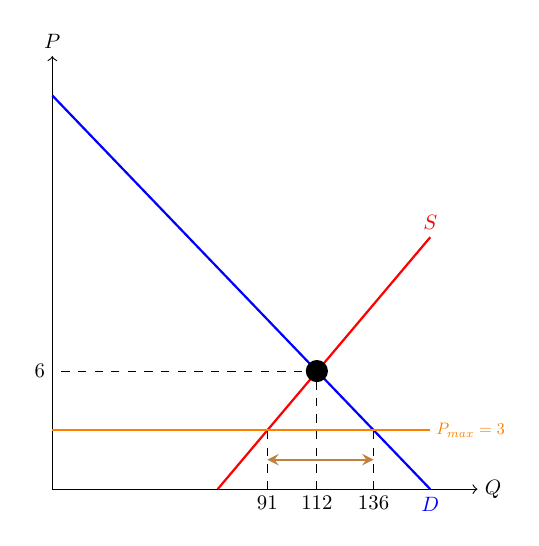
\begin{tikzpicture}[x=0.3cm, y=0.25cm, every node/.style={scale=0.75}]
						% 坐标轴
						\draw[->] (0,0) -- (18,0) node[right] {$Q$};
						\draw[->] (0,0) -- (0,22) node[above] {$P$};
						% 需求曲线 P = 20 - 0.125Q (Q=160, P=20)
						\draw[thick, blue] (0,20) -- (16,0) node[below] {$D$};
						% 供给曲线 P = (Q-70)/7 (Q=160, P~12.8)
						\draw[thick, red] (7,0) -- (16,12.8) node[above] {$S$};
						% 均衡点 E(112, 6)
						\draw[dashed] (11.2,0) node[below] {112} -- (11.2,6) -- (0,6) node[left] {6};
						\fill (11.2,6) circle (4pt);
						% 租金上限 P=3
						\draw[thick, orange] (0,3) -- (16,3) node[right, scale=0.8] {$P_{max}=3$};
						\draw[dashed] (9.1,0) node[below] {91} -- (9.1,3);
						\draw[dashed] (13.6,0) node[below] {136} -- (13.6,3);
						% 短缺箭头
						\draw[<->, >=stealth, thick, brown] (9.1,1.5) -- (13.6,1.5);
					\end{tikzpicture}
					
					\vspace{0.5em}
					{\small (a) 租金上限与短缺}
				\end{minipage}%
				\hfill
				\begin{minipage}[t]{0.48\textwidth}
					\centering
					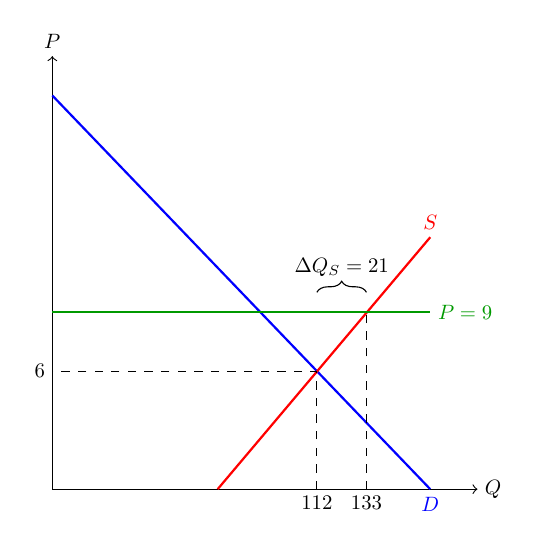
\begin{tikzpicture}[x=0.3cm, y=0.25cm, every node/.style={scale=0.75}]
						% 坐标轴
						\draw[->] (0,0) -- (18,0) node[right] {$Q$};
						\draw[->] (0,0) -- (0,22) node[above] {$P$};
						% 需求与供给
						\draw[thick, blue] (0,20) -- (16,0) node[below] {$D$};
						\draw[thick, red] (7,0) -- (16,12.8) node[above] {$S$};
						% 原均衡点参考
						\draw[dashed, black] (11.2,0) node[below] {112} -- (11.2,6) -- (0,6) node[left] {6};
						% 价格设定 P=9
						\draw[thick, green!60!black] (0,9) -- (16,9) node[right] {$P=9$};
						\draw[dashed] (13.3,0) node[below] {133} -- (13.3,9);
						% 供给增量括号
						\draw[decorate, decoration={brace, amplitude=4pt}] (11.2,10) -- (13.3,10) node[midway, above=4pt] {$\Delta Q_S=21$};
					\end{tikzpicture}
					
					\vspace{0.5em}
					{\small (b) 租金上升与供给增加}
				\end{minipage}
			\end{center}
			
			\newpage
			\item \textbf{2010年，美国人总共消费了3150亿支香烟，合157.5亿包。香烟的每包零售价（含税）大约平均为5美元。统计研究表明，需求的价格弹性是$-0.4$，供给的价格弹性是$0.5$。}
			
			\textbf{(a)根据这些信息，请推导香烟市场的线性需求曲线和线性供给曲线。}
			
			\textbf{答：}
			首先明确线性供需曲线的通用形式：
				$$ \text{需求曲线：} Q_d = a - bP $$
				$$ \text{供给曲线：} Q_s = c + dP $$
			
			根据已知均衡点 $Q^* = 157.5$，$P^* = 5$，推导过程如下：
			
			1. 求解需求曲线 \\
			利用点弹性公式 $$E_d = \frac{dQ_d}{dP} \cdot \frac{P^*}{Q^*}$$
			代入数据：
			$$ -0.4 = -b \cdot \frac{5}{157.5} \implies b = 12.6 $$
			将均衡点代入需求方程求解截距 $a = 220.5$\\
			得线性需求曲线为：$Q_d = 220.5 - 12.6P$。
			
			2. 求解供给曲线 \\
			利用点弹性公式 $$E_s = \frac{dQ_s}{dP} \cdot \frac{P^*}{Q^*}$$
			代入数据：
			$$ 0.5 = d \cdot \frac{5}{157.5} \implies d = 15.75 $$
			将均衡点代入供给方程求解截距 $c = 78.75$\\
			得线性供给曲线为：$\boldsymbol{Q_s = 78.75 + 15.75P}$。
			
			 \textbf{(b)1998年，美国人共消费了235亿包香烟，每包零售价为2美元。1998—2010年，香烟消费下降的部分原因是人们更多地认识到吸烟对健康的危害，部分原因是价格的上升。假设消费下降的所有原因都是价格上升，你可以推断出需求的价格弹性具有什么特征吗？}
			
			若假定消费下降完全由价格上涨导致，则意味着需求曲线未发生位移，观测到的变动完全是沿着同一条需求曲线的点移动。基于此假设，我们计算需求弧弹性：

				$$ E_d = \frac{\Delta Q}{\Delta P} \cdot \frac{(P_1 + P_2)/2}{(Q_1 + Q_2)/2} $$
			
			已知 1998 年数据为 $(P_1, Q_1) = (2, 235)$，2010 年数据为 $(P_2, Q_2) = (5, 157.5)$：
			$$ \Delta Q = 157.5 - 235 = -77.5, \quad \Delta P = 5 - 2 = 3 $$
			代入弧弹性公式：
			$$ \begin{aligned}
				E_d &= \frac{-77.5}{3} \cdot \frac{(2 + 5)/2}{(235 + 157.5)/2} \\
				& \approx -0.46
			\end{aligned} $$
			
			根据计算结果，可以推断该需求具有以下特征：
			\begin{enumerate}
				\item \textbf{需求缺乏弹性}：由于 $|E_d| \approx 0.46 < 1$，香烟需求表现为缺乏弹性。这意味着价格大幅上升仅引起消费量较小幅度的下降。
				\item \textbf{刚需属性}：长期来看，即便将所有消费降幅归结为价格因素，弹性系数依旧偏低。这印证了香烟作为成瘾性商品，消费者对其价格敏感度较低。
				\item \textbf{长期与短期的差异}：对比 2010 年的短期点弹性（$-0.4$）与该长期弧弹性（约 $-0.46$），可以看出随着时间推移，消费者通过调整习惯等方式，对价格的反应会比短期稍微灵敏一些。
			\end{enumerate}

			\item \textbf{在例2.8中，通过第2.6节中推导出来的线性供给曲线和线性需求曲线，我们研究了铜的需求量下降20\%对铜价的影响。假设铜的长期价格弹性是$-0.75$，而非$-0.5$。例题已知初始条件：铜的供给曲线 $Q_s = -9 + 9P$；初始均衡价格 $P^* = 3$ 美元/磅，均衡数量 $Q^* = 18$ 百万公吨/年。}
			
			\begin{enumerate}[label=\textbf{\alph*.}, leftmargin=2em]
				\item \textbf{如前假定，均衡价格和数量为 $P^* = 3$ 美元/磅，$Q^* = 18$ 百万公吨/年，试推导出与更小的需求弹性相一致的线性需求曲线。}
				\item \textbf{运用这一需求曲线，重新计算铜的需求下降55\%对铜价的影响。}
			\end{enumerate}
			
			\textbf{答：}
			
			\textbf{a.} 首先推导新的线性需求曲线。设线性需求曲线为：
				$$ Q_d = a - bP $$
			
			根据需求价格点弹性的定义公式 
			$$E_d = \frac{dQ_d}{dP} \cdot \frac{P}{Q}$$
			将已知的均衡点 $(P^*, Q^*) = (3, 18)$ 以及新的需求价格弹性 $E_d = -0.75$ 代入公式计算：
			$$ -0.75 = -b \cdot \frac{3}{18} $$
			解得 $b = 4.5$。
			
			接着，将市场均衡点和求得的斜率系数代入需求曲线方程，得解截距 $a = 31.5 $

			因此，与更小需求弹性相一致的新线性需求曲线方程为：
			$$ Q_d = 31.5 - 4.5P $$
			
			\vspace{1em}
			
			\textbf{b.} 接下来重新计算铜的需求下降 $55\%$ 对铜价的影响。
			
			当铜的市场需求整体下降 $55\%$ 时，意味着在任何既定的价格水平下，新的需求量仅为原需求量的 $45\%$。基于此，我们推导新的需求曲线方程：
				$$ Q_d' = 0.45 \times (31.5 - 4.5P) = 14.175 - 2.025P $$
			
			已知短期内铜的供给曲线保持不变，仍为 $Q_s = -9 + 9P$。在新的市场均衡状态下，供给量等于变动后的需求量（即 $Q_s = Q_d'$）。联立供需方程求解新的均衡价格：
			$$ \begin{aligned}
				-9 + 9P &= 14.175 - 2.025P \\
				P' &\approx 2.10
			\end{aligned} $$
			
			最后分析价格的变动幅度。初始均衡价格为 $P^* = 3$ 美元/磅，在需求大幅下降 $55\%$ 后，市场均衡价格跌至约 $2.10$ 美元/磅。对应的价格下跌幅度为：
			$$ \frac{3 - 2.10}{3} \times 100\% = 30\% $$
			
			由此可见，当长期的需求变得更加缺乏弹性时，需求量的大幅下降最终会导致铜的市场均衡价格出现显著下跌（降幅达 $30\%$）。
			
			\item \textbf{我们在例2.8中讨论了近几年铜的全球需求的下降，部分归因于中国不断下降的消费。不过，如果中国的需求上升了会怎么样呢？已知初始需求曲线 $Q_D = 27 - 3P$，初始供给曲线 $Q_S = -9 + 9P$；初始均衡价格 $P^* = 3$ 美元/磅，$Q^* = 18$ 百万公吨/年。}
			
			\begin{enumerate}[label=\textbf{\alph*.}, leftmargin=2em]
				\item \textbf{利用初始的需求弹性和供给弹性（即 $E_S = 1.5$ 且 $E_D = -0.5$），计算铜的需求增加20\%对铜价的影响。}
				\item \textbf{计算该需求增加对均衡数量 $Q^*$ 的影响。}
				\item \textbf{正如我们在例2.8中所讨论的，美国铜产量在2000—2003年下降了。计算铜的需求增加20\%且铜的供给下降20\%对均衡价格和产量的影响。}
			\end{enumerate}
			
			\textbf{答：}
			
			\textbf{a.} 当铜的需求整体增加 $20\%$ 时，意味着在任意既定价格下，新需求量变为原需求量的 $1.2$ 倍。推导新需求曲线如下：
				$$ Q_D' = 1.2 \times (27 - 3P) = 32.4 - 3.6P $$
			在短期供给曲线不变（$Q_S = -9 + 9P$）的情况下，联立新的供需方程求解新均衡价格 $P'$：
			$$ \begin{aligned}
				32.4 - 3.6P &= -9 + 9P \\
				P' &\approx 3.29 \text{ 美元/磅}
			\end{aligned} $$
			由此可见，需求增加 $20\%$ 会导致铜的均衡价格从 $3$ 美元上涨至约 $3.29$ 美元/磅。
			
			\vspace{1em}
			\textbf{b.} 将求得的新均衡价格 $P' \approx 3.29$ 代入供给曲线，计算新的均衡数量 $Q'$：
			$$ Q' = -9 + 9 \times 3.29 \approx 20.61 \text{ 百万公吨/年} $$
			均衡数量的变动量为 $\Delta Q = 20.61 - 18 = 2.61 \text{ 百万公吨/年}$。这意味着均衡产量较初始水平提升了约 $14.5\%$。
			
			\vspace{1em}
			\textbf{c.} 当铜的供给整体下降 $20\%$ 时，新的供给量变为原供给量的 $0.8$ 倍。推导新供给曲线如下：
			
				$$ Q_S' = 0.8 \times (-9 + 9P) = -7.2 + 7.2P $$
				
			结合 a 问中右移的新需求曲线 $Q_D' = 32.4 - 3.6P$，再次联立求解全新的市场均衡：
			$$ \begin{aligned}
				32.4 - 3.6P &= -7.2 + 7.2P \\
				P'' &\approx 3.67 \text{ 美元/磅}
			\end{aligned} $$
			将 $P''$ 代入新供给曲线求均衡数量：
			$$ Q'' = -7.2 + 7.2 \times 3.67 \approx 19.22 \text{ 百万公吨/年} $$
			结论：在需求增加 $20\%$ 且供给减少 $20\%$ 的双重冲击下，铜的供不应求状况加剧，均衡价格将进一步推高至约 $3.67$ 美元/磅，而均衡产量变为约 $19.22$ 百万公吨/年。
			
			\newpage
			
			\item \textbf{例2.9分析了世界石油市场。利用该例所提供的数据：}
			\begin{enumerate}[label=\textbf{\alph*.}, leftmargin=2em]
				\item \textbf{证明短期需求曲线和竞争性供给曲线的确是如下形式：$D = 36.75 - 0.035P$，$S_C = 21.85 + 0.023P$}
				\item \textbf{证明长期需求曲线和竞争性供给曲线的确是如下形式：$D = 45.5 - 0.210P$，$S_C = 16.1 + 0.138P$}
				\item \textbf{在例2.9中，我们考察了沙特阿拉伯的石油减产对石油价格的影响。假设由于沙特阿拉伯开发了新油田，从而欧佩克（OPEC）的产量每年增加20亿桶。计算石油产量增加对短期和长期石油价格的影响。}
			\end{enumerate}
			
			\textbf{答：}
			
			\textbf{a.} 根据原例题数据，世界石油市场初始短期均衡价格 $P=50$ 美元/桶，总需求 $Q=35$ 十亿桶/年；短期需求价格弹性 $E_D = -0.05$。
			设短期线性需求曲线为 $D = a - bP$。由点弹性公式推导斜率 $-b$：
			$$ E_D = -b \cdot \frac{P}{Q} \implies b = 0.035 $$
			代入均衡点求截距 $a$：
			$$ 35 = a - 0.035 \times 50 \implies a = 36.75 $$
			因此，短期需求曲线证明为 $D = 36.75 - 0.035P$。
			
			对于短期竞争性供给曲线 $S_C = c + dP$（已知短期竞争性供给弹性 $E_S = 0.05$），若按照给定系数 $d = 0.023$ 反向验证：
			将 $P=50$ 代入目标方程 $S_C = 21.85 + 0.023P$，得非欧佩克竞争性供给量 $S_C = 23$。此时加上欧佩克设定的固定产量（$12$ 十亿桶），总供给刚好为 $23 + 12 = 35$，符合市场出清条件，曲线得证。(也可以用弹性定义求)
			
			\vspace{1em}
			\textbf{b.} 根据例题长期数据，长期需求价格弹性 $E_D = -0.3$。
			设长期线性需求曲线为 $D = a - bP$。推导斜率 $-b$：
			$$ E_D = -b \cdot \frac{P}{Q} \implies b = 0.210 $$
			代入均衡点求截距 $a$：
			$$ 35 = a - 0.210 \times 50 \implies a = 45.5 $$
			因此，长期需求曲线证明为 $D = 45.5 - 0.210P$。
			
			设长期竞争性供给曲线为 $S_C = c + dP$。已知欧佩克产量为 $12$，故市场对竞争性供给的需求为 $23$。若按给定方程验证：
			将 $P=50$ 代入 $S_C = 16.1 + 0.138P$，得到 $S_C = 23$。这与长期供给弹性设定的理论值高度吻合，曲线得证。(也可以用弹性定义求)
			
			\vspace{1em}
			\textbf{c.}当欧佩克产量每年增加 $20$ 亿桶时，意味着其固定供给量由原先的 $12$ 十亿桶/年增加至 $14$ 十亿桶/年。全新的世界总供给曲线变为 $S_T = S_C + 14$。
			
			短期油价影响计算：
			新的短期总供给曲线为：
			$$ S_{T} = (21.85 + 0.023P) + 14 = 35.85 + 0.023P $$
			联立短期供需均衡条件 $S_{T} = D$：
				$$ 35.85 + 0.023P = 36.75 - 0.035P $$
			$$ \implies P \approx 15.52 \text{ 美元/桶} $$
			短期内由于供需双侧均极度缺乏弹性，即便只是 $20$ 亿桶的产能释放，也会导致市场严重供过于求，迫使石油价格从初始的 $50$ 美元/桶大幅暴跌至约 $15.52$ 美元/桶。
			
			长期油价影响计算：
			新的长期总供给曲线为：
			$$ S_{T} = (16.1 + 0.138P) + 14 = 30.1 + 0.138P $$
			联立长期供需均衡条件 $S_{T} = D$：
				$$ 30.1 + 0.138P = 45.5 - 0.210P $$
			$$  \implies P \approx 44.25 \text{ 美元/桶} $$
			结论：长期来看，需求和非欧佩克供给变得更加富有弹性，市场自我调节与吸收过剩产能的能力显著增强。因此石油价格会有所回升，长期均衡价格将稳定在约 $44.25$ 美元/桶，相比初始的 $50$ 美元/桶仅呈现温和下跌。
			
			\item \textbf{参见例2.10，该例分析了价格控制对天然气的影响。a. 利用该例中的数据，证明下述供给曲线和需求曲线的确描述了2005—2007年的市场：供给：$Q=15.90+0.72P_G+0.05P_O$，需求：$Q=0.02-1.8P_G+0.69P_O$。其中，$P_G$和$P_O$分别是天然气和石油的价格。另外请证实，如果石油价格为50美元，这些曲线意味着天然气的自由市场价格为6.40美元。b. 假设天然气的调控价格是4.50美元/千立方英尺，而非3美元/千立方英尺，那么超额需求会是多少？c. 假设天然气的市场并没有受到调控，如果石油价格从50美元涨至100美元，天然气的自由市场价格又将会发生什么变化？}
			
			\textbf{答：}
			本题已知2005-2007年天然气市场基准均衡数据：
			
			均衡数量 $Q=23$ 万亿立方英尺，天然气均衡价格 $P_G=6.40$ 美元/千立方英尺，石油价格 $P_O=50$ 美元/桶；核心弹性数据：天然气需求价格弹性 $E_d=-0.5$，供给价格弹性 $E_s=0.2$，天然气需求对石油的交叉价格弹性 $E_{d,PO}=1.5$，供给对石油的交叉价格弹性 $E_{s,PO}=0.1$。
			
			线性曲线点弹性核心公式如下：
				$$E = \frac{dQ}{dP} \cdot \frac{P}{Q}$$
			
			a. 
			
			步骤1：推导需求曲线\\
			线性需求曲线形式为 $Q_D = a - bP_G + fP_O$
			
			代入需求价格弹性公式：
			$$E_d = -b \cdot \frac{P_G}{Q} = -0.5$$
			解得 $b \approx 1.8$
	
			代入交叉价格弹性公式：
			$$E_{d,PO} = f \cdot \frac{P_O}{Q} = 1.5$$
			解得 $f = 0.69$
			
			将均衡数据、$b=1.8$、$f=0.69$ 代入需求方程：
			$$23 = a - 1.8 \times 6.40 + 0.69 \times 50$$
			解得 $a = 0.02$
			
			最终需求曲线如下：
				$$Q_D = 0.02 - 1.8P_G + 0.69P_O$$
			
			\newpage
			步骤2：推导供给曲线\\
			线性供给曲线形式为 $Q_S = c + dP_G + eP_O$

			代入供给价格弹性公式：
			$$E_s = d \cdot \frac{P_G}{Q} = 0.2$$
			解得 $d \approx 0.72$
			
			代入交叉价格弹性公式：
			$$E_{s,PO} = e \cdot \frac{P_O}{Q} = 0.1$$
			解得 $e = 0.05$
			
			将均衡数据、$d=0.72$、$e=0.05$ 代入供给方程：
			$$23 = c + 0.72 \times 6.40 + 0.05 \times 50$$
			解得 $c \approx 15.90$
			最终供给曲线如下：

				$$Q_S = 15.90 + 0.72P_G + 0.05P_O$$
			
			步骤3：验证自由市场均衡价格\\
			令 $Q_S=Q_D$，代入 $P_O=50$ 美元/桶：
			$$15.90 + 0.72P_G + 0.05 \times 50 = 0.02 - 1.8P_G + 0.69 \times 50$$ 
			$$P_G \approx 6.40$$
			
			b. 调控价格 4.50 美元/千立方英尺时的超额需求
			
			将 $P_G=4.50$、$P_O=50$ 代入供需曲线：
			$$Q_S = 15.90 + 0.72 \times 4.50 + 0.05 \times 50 = 21.64$$
			$$Q_D = 0.02 - 1.8 \times 4.50 + 0.69 \times 50 = 26.42$$
			超额需求的计算如下：
				$$\text{超额需求} = Q_D - Q_S = 26.42 - 21.64 = 4.78 \text{ 万亿立方英尺}$$
			
			c. 石油价格涨至 100 美元/桶的市场变化
			
			求新的自由市场均衡：令 $Q_S=Q_D$，代入 $P_O=100$ 美元/桶：
				$$
				\begin{aligned}
					15.90 + 0.72P_G + 0.05 \times 100 &= 0.02 - 1.8P_G + 0.69 \times 100 \\
					P_G &\approx 19.10 \text{ 美元/千立方英尺}
				\end{aligned}
				$$
			石油价格翻倍后，天然气的自由市场均衡价格从 6.40 大幅上涨至约 19.10 美元/千立方英尺，涨幅近200\%。
			\newpage
			\item \textbf{下表显示的是速溶咖啡和烘焙咖啡两年中的零售价格和销售量。a. 使用下面的数据，估计烘焙咖啡需求的短期价格弹性，并推导烘焙咖啡的线性需求曲线。b. 估计速溶咖啡需求的短期价格弹性，并推导速溶咖啡的线性需求曲线。c. 哪一种咖啡的短期需求价格弹性大一些？你认为这是什么原因？}
			
			\begin{center}
				\renewcommand{\tabularxcolumn}[1]{m{#1}}
				\begin{tabularx}{\textwidth}{>{\centering\arraybackslash}X >{\centering\arraybackslash}X >{\centering\arraybackslash}X >{\centering\arraybackslash}X >{\centering\arraybackslash}X}
					\toprule
					\textbf{年份} & \textbf{速溶咖啡零售价格（美元/磅）} & \textbf{速溶咖啡销售量（百万磅）} & \textbf{烘焙咖啡零售价格（美元/磅）} & \textbf{烘焙咖啡销售量（百万磅）} \\
					\midrule
					第一年 & 10.35 & 75 & 4.11 & 820 \\
					第二年 & 10.48 & 70 & 3.76 & 850 \\
					\bottomrule
				\end{tabularx}
			\end{center}
			
			\textbf{答：}
			本题采用短期弧弹性计算，线性需求曲线通用形式为 $Q = a - bP$
			弹性核心公式如下：
				$$E_d = \frac{\Delta Q / Q_1}{\Delta P / P_1}$$
			其中 $Q_1$、$P_1$ 为第一年的销量与价格。
			
			a. 烘焙咖啡的需求价格弹性与线性需求曲线\\
			已知烘焙咖啡数据：$P_1=4.11$，$Q_1=820$；$P_2=3.76$，$Q_2=850$\\

			$$E_d = \frac{(Q_2-Q_1)/Q_1}{(P_2-P_1)/P_1}\approx -0.43$$

			斜率 $b \approx 85.71$
			代入第一年数据求截距 $a$：
			$$820 = a - 85.71 \times 4.11$$
			解得 $a \approx 1172.27$。最终线性需求曲线如下：
				$$Q = 1172.27 - 85.71P$$

			
			b. 速溶咖啡的需求价格弹性与线性需求曲线\\
			已知速溶咖啡数据：$P_1=10.35$，$Q_1=75$；$P_2=10.48$，$Q_2=70$

			$$E_d = \frac{(Q_2-Q_1)/Q_1}{(P_2-P_1)/P_1} \approx -5.29$$

			斜率 $b \approx 38.46$
			代入第一年数据求截距 $a$：
			$$75 = a - 38.46 \times 10.35$$
			解得 $a \approx 473.06$。最终线性需求曲线如下：
				$$Q = 473.06 - 38.46P$$

			c. 弹性对比与原因\\
			速溶咖啡的短期需求价格弹性远大于烘焙咖啡。可能的原因是：速溶咖啡产品同质化程度高，市场上可替代的饮品、品牌丰富，消费者对价格变动的敏感度更高；烘焙咖啡（现磨/现煮咖啡）具有更强的消费黏性、品牌与品质偏好，日常刚需属性更突出，消费者对其价格变动的容忍度更高，因此需求对价格变化的反应更小。
		\end{enumerate}
	% =======================================================
	%                   第 3 章：消费者行为
	% =======================================================
	\chapter{消费者行为}
	
	\section{复习题}
		\begin{enumerate}[label=\textbf{\arabic*.}, leftmargin=*]
			\item \textbf{个人偏好的四个基本假设是什么？}
			
			\textbf{答：}
			个人偏好的四个基本假设是构建理性消费者行为理论的基础。
				$$ A \succ B \quad \text{（严格偏好）}, \quad A \sim B \quad \text{（无差异）} $$
			
			假设如下：
			\begin{enumerate}
				\item 完备性：消费者能对任意两个商品组合 $A$、$B$ 进行明确排序，要么 $A \succ B$，要么 $B \succ A$，要么 $A \sim B$，不存在无法比较的情况。
				\item 传递性：若 $A \succ B$ 且 $B \succ C$，则必有 $A \succ C$。这保证了偏好的一致性，避免循环矛盾。
				\item 单调性（非餍足性）：对正常商品，消费者总是偏好数量更多的组合。若组合 $A$ 中商品数量不小于 $B$，且至少一种商品数量严格大于 $B$，则 $A \succ B$。当消费超过餍足点后，商品会转变为厌恶品，此时“越多越好”不再成立。
				\item 凸性：偏好是凸的，即两个无差异组合的加权平均，至少与原组合一样好。这等价于边际替代率递减，保证无差异曲线凸向原点。
			\end{enumerate}
			
			四个基本假设的直观图示如下：
			\begin{center}
				\begin{tikzpicture}[scale=0.85, every node/.style={scale=0.9}]
					% 1. 完备性
					\begin{scope}[xshift=0cm]
						\draw[->] (0,0) -- (3.2,0) node[right] {$x_1$};
						\draw[->] (0,0) -- (0,3.2) node[above] {$x_2$};
						\fill (1,1) circle (2pt) node[below left] {$A$};
						\fill (2.2,2.2) circle (2pt) node[above right] {$B$};
						% 缩短箭头并倾斜文本以防止字体遮挡
						\draw[thick,->,red,shorten >=3pt,shorten <=3pt] (1,1) -- (2.2,2.2) node[midway,sloped,above] {$A \prec B$};
						\node[below] at (1.5,-0.5) {完备性};
					\end{scope}
					
					% 2. 传递性
					\begin{scope}[xshift=4.5cm]
						\draw[->] (0,0) -- (3.2,0) node[right] {$x_1$};
						\draw[->] (0,0) -- (0,3.2) node[above] {$x_2$};
						\fill (0.6,0.6) circle (2pt) node[below right] {$C$};
						\fill (1.4,1.4) circle (2pt) node[below right] {$B$};
						\fill (2.2,2.2) circle (2pt) node[above left] {$A$};
						\draw[thick,->,blue,shorten >=3pt,shorten <=3pt] (0.6,0.6) -- (1.4,1.4);
						\draw[thick,->,blue,shorten >=3pt,shorten <=3pt] (1.4,1.4) -- (2.2,2.2);
						% 增加辅助虚线和斜向文本展示传递结果
						\draw[thick,->,blue,dashed,shorten >=3pt,shorten <=3pt] (0.6,0.6) to[bend left=20] node[midway,sloped,above] {$C \prec A$} (2.2,2.2);
						\node[below] at (1.5,-0.5) {传递性};
					\end{scope}
					
					% 3. 单调性（非餍足性）
					\begin{scope}[xshift=9cm]
						\draw[->] (0,0) -- (3.2,0) node[right] {$x_1$};
						\draw[->] (0,0) -- (0,3.2) node[above] {$x_2$};
						\fill (1.2,1.2) circle (2pt) node[below left] {$B$};
						\fill (2.2,2.2) circle (2pt) node[above right] {$A$};
						% 增加阴影区域直观展示非餍足性特征
						\fill[green!10, opacity=0.7] (1.2,1.2) rectangle (3.0,3.0);
						\draw[dashed] (1.2,1.2) -- (3.0,1.2);
						\draw[dashed] (1.2,1.2) -- (1.2,3.0);
						\draw[thick,->,green!60!black,shorten >=3pt,shorten <=3pt] (1.2,1.2) -- (2.2,2.2) node[midway,sloped,below] {$A \succ B$};
						\node[below] at (1.5,-0.5) {单调性};
					\end{scope}
					
					% 4. 凸性（无差异曲线凸向原点）
					\begin{scope}[xshift=13.5cm]
						\draw[->] (0,0) -- (3.2,0) node[right] {$x_1$};
						\draw[->] (0,0) -- (0,3.2) node[above] {$x_2$};
						
						% 绘制真正严格凸向原点的无差异曲线 (双曲线 y = 1.7/x)
						\draw[thick, domain=0.6:2.8, samples=50] plot (\x, {1.7/\x}) node[below] {$U_1$};
						
						% 定义位于曲线上的两点及其连线中点
						\coordinate (X) at (0.7, 2.428);
						\coordinate (Y) at (2.428, 0.7);
						\coordinate (Z) at (1.564, 1.564); % (X+Y)/2 中点
						
						% 绘制连线及点
						\draw[dashed] (X) -- (Y);
						\fill (X) circle (2pt) node[above right] {$X$};
						\fill (Y) circle (2pt) node[above right] {$Y$};
						\fill (Z) circle (2pt) node[above right] {$Z$};
						
				        % 延伸 U2 曲线的 domain 到 3.0，使 label 右移，远离点 Y 及其标注
				        \draw[dashed, gray, domain=0.8:3.3, samples=50] plot (\x, {2.446/\x}) node[right] {$U_2$};
						
						\node[below] at (1.5,-0.5) {凸性};
					\end{scope}
				\end{tikzpicture}
			\end{center}
			
			\item \textbf{一组正常商品的无差异曲线能否向上倾斜？试说明理由。}
			
			\textbf{答：}
			对于正常商品而言，无差异曲线不能向上倾斜。其逻辑矛盾可以通过偏好的基本假设进行证明：
				$$ \text{假设 } A, B \text{ 位于同一条向上倾斜的 } U \implies U(A) = U(B) $$
				$$ \text{若 } B \text{ 位于 } A \text{ 的右上方，则 } B > A \implies U(B) > U(A) \quad (\text{单调性假设}) $$
			上述结论直接违背了单调性（非餍足性）假设，即消费者总是偏好数量更多的商品组合。
			
			若其中一种商品为厌恶品（如噪音、空气污染），为了抵消厌物品带来的效用损失，必须增加另一种正常商品的消费以维持原有效用，此时无差异曲线会向上倾斜。此外，若存在餍足点，当消费量超过该点后，商品转变为厌恶品，无差异曲线将呈现围绕餍足点的闭合环状。
			
			\begin{center}
				\begin{tikzpicture}[scale=0.85, every node/.style={scale=0.9}]
					% 左图：向上倾斜的矛盾
					\begin{scope}[xshift=0cm]
						\draw[->] (0,0) -- (3.5,0) node[right] {$x_1$};
						\draw[->] (0,0) -- (0,3.5) node[above] {$x_2$};
						% 绘制向上倾斜的无差异曲线
						\draw[thick, red] (0.5,0.5) -- (3,3) node[right] {$U$};
						\fill (1,1) circle (2pt) node[below right] {$A$};
						\fill (2.2,2.2) circle (2pt) node[above left] {$B$};
						
						% 采用参考画法：增加阴影区域与虚线边界直观展示更优区域
						\fill[green!10, opacity=0.7] (1,1) rectangle (3.2,3.2);
						\draw[dashed] (1,1) -- (3.2,1);
						\draw[dashed] (1,1) -- (1,3.2);
						\node[green!60!black, font=\bfseries] at (2.4,1.4) {更优区域};
						
						\node[below] at (1.75,-0.6) {违背单调性};
					\end{scope}
					
					% 右图：厌物品/餍足点
					\begin{scope}[xshift=6cm]
						\draw[->] (0,0) -- (3.5,0) node[right] {$x_1$};
						\draw[->] (0,0) -- (0,3.5) node[above] {$x_2$};
						\coordinate (S) at (1.75,1.75);
						\fill (S) circle (2pt); 
						% 绘制环状无差异曲线
						\draw[thick, blue!70] (S) circle (0.6);
						\draw[thick, blue!50] (S) circle (1.1);
						\draw[thick, blue!30] (S) circle (1.6);
						% 从圆心拉出箭头指向外部空白处
						\node (satiation_text) at (4.2, 2.8) {餍足点};
						\draw[->, >=stealth, dashed, gray] (S) -- (satiation_text);
						\node[below] at (1.75,-0.6) {环状无差异曲线};
					\end{scope}
				\end{tikzpicture}
			\end{center}
			
			\item \textbf{解释两条无差异曲线为什么不能相交。}
			
			\textbf{答：}
			两条无差异曲线相交会同时违背偏好的传递性与单调性假设。证明如下：

				$$ \begin{cases} A \sim B \quad (\text{均在无差异曲线 } U_2 \text{ 上}) \\ A \sim C \quad (\text{均在无差异曲线 } U_1 \text{ 上}) \end{cases} \implies B \sim C \quad (\text{传递性}) $$
				$$ \text{观察图示：} B \text{ 位于 } C \text{ 的右上方 } \implies B > C \implies B \succ C \quad (\text{单调性}) $$

			由于逻辑推导出的“无差异”与观察事实得出的“偏好”产生了矛盾，因此两条无差异曲线在同一偏好体系下绝不可能相交。
			
			\begin{center}
				\begin{tikzpicture}[scale=1.2, every node/.style={scale=0.9}]
					\draw[->] (0,0) -- (4.5,0) node[right] {$x_1$};
					\draw[->] (0,0) -- (0,4.5) node[above] {$x_2$};
					
					% 重新设计曲线函数，确保夹角足够大且点绝对落在曲线上
					% U1: y = 4/x (蓝色)
					\draw[thick, blue, domain=1:4.2, samples=100] plot (\x, {4/\x}) node[right] {$U_1$};
					% U2: y = 1.5/x + 1.5 (红色)
					\draw[thick, red, domain=0.6:4.2, samples=100] plot (\x, {1.5/\x + 1.5}) node[right] {$U_2$};
					
					% 交点 A 位于 (1.667, 2.4)，精确计算保证在曲线上
					\coordinate (A) at (1.667, 2.4);
					\fill (A) circle (1.8pt) node[below left] {$A$};
					
					% 取点 C 和 B，直接使用数学函数坐标确保绝对在线上
					% 点 C 位于 U1 上，设 x=2.8，y = 4/2.8 = 1.428
					\coordinate (C) at (2.8, {4/2.8});
					% 点 B 位于 U2 上，设 x=3.5，y = 1.5/3.5 + 1.5 = 1.928
					\coordinate (B) at (3.5, {1.5/3.5 + 1.5});
					
					\fill (B) circle (1.8pt) node[above right] {$B$};
					\fill (C) circle (1.8pt) node[below left] {$C$};
					
					% 绘制辅助虚线，清晰展示 B 完全处于 C 的右上方（x、y均更大）
					\draw[dashed, gray!80] (C) -| (B);
					\node[gray, font=\tiny] at (3.15, 1.6) {$\Delta > 0$};
					
					\node at (2.25, -0.6) {相交无差异曲线的矛盾};
				\end{tikzpicture}
			\end{center}
			
			\item \textbf{乔恩总是愿意以一听可口可乐换取一听雪碧，或者以一听雪碧换取一听可口可乐。\\ a. 你如何看待乔恩的边际替代率？\\ b. 画出乔恩的一组无差异曲线。\\ c. 画出两条斜率不一样的预算线，并说明效用最大化的选择。从中你能得出什么结论？}
			
			\textbf{答：}
			
			a. 边际替代率（$MRS$）衡量消费者在维持效用不变的前提下，愿意用一种商品交换另一种商品的比例。

				$$MRS_{xy} = - \frac{\Delta y}{\Delta x} = 1$$

			由于乔恩认为一听可口可乐与一听雪碧在效用上是完全等同的（1:1 交换），这意味着两种商品对他而言是完全替代品。因此，他的边际替代率是一个常数，且恒等于 $1$。
			
			b. 对于完全替代品，其效用函数可表示为 $U(x, y) = ax + by$。在本题中，$a=b=1$，即 $U = x + y$。其无差异曲线是一组斜率为 $-1$ 的平行直线。
			
			c. 效用最大化的选择取决于预算线的斜率（即相对价格比 $P_x/P_y$）与无差异曲线斜率（$MRS$）的比较。
			
			对于完全替代品，消费者的最优决策通常表现为角点解，即消费者会将其全部收入集中用于购买价格相对较低的那种商品，以实现效用最大化。

			\begin{center}
				\begin{tikzpicture}[scale=1.2, every node/.style={scale=0.9}]
					% --- 图 (1): 无差异曲线 (仅一条线表示 U=x+y) ---
					\begin{scope}[xshift=0cm]
						\draw[->] (0,0) -- (3,0) node[right] {雪碧 ($x$)};
						\draw[->] (0,0) -- (0,3) node[above] {可乐 ($y$)};
						% 无差异曲线: x + y = 2.5
						\draw[thick, blue] (0,2.5) -- (2.5,0) node[above right] {$U$};
						\node[below] at (1.5,-0.5) {(1) 无差异曲线 $U=x+y$};
					\end{scope}
					
					% --- 图 (2): 价格低的情况 (Px < Py) ---
					\begin{scope}[xshift=4.5cm]
						\draw[->] (0,0) -- (3,0) node[right] {$x$};
						\draw[->] (0,0) -- (0,3) node[above] {$y$};
						% 相同的无差异曲线 (蓝色)
						\draw[thick, blue] (0,2.5) -- (2.5,0);
						% 预算线 (红色): 较平缓 (斜率 < 1)，且在 x 轴与无差异曲线交于同一点
						% 设预算线为 y = 1.5 - 0.6x，则 x 截距为 2.5
						\draw[thick, red] (0,1.5) -- (2.5,0);
						% 标注最优解
						\fill[red] (2.5,0) circle (2pt);
						\node[below] at (2.5,0) {\small 最优解};
						\node[below] at (1.5,-0.5) {(2) $P_x < P_y$ (全部买 $x$)};
					\end{scope}
					
					% --- 图 (3): 价格高的情况 (Px > Py) ---
					\begin{scope}[xshift=9cm]
						\draw[->] (0,0) -- (3,0) node[right] {$x$};
						\draw[->] (0,0) -- (0,3) node[above] {$y$};
						% 相同的无差异曲线 (蓝色)
						\draw[thick, blue] (0,2.5) -- (2.5,0);
						% 预算线 (红色): 较陡峭 (斜率 > 1)，且在 y 轴与无差异曲线交于同一点
						% 设预算线为 y = 2.5 - 1.6x，则 y 截距为 2.5
						\draw[thick, red] (0,2.5) -- (1.56,0);
						% 标注最优解
						\fill[red] (0,2.5) circle (2pt);
						\node[left] at (0,2.5) {\small 最优解};
						\node[below] at (1.5,-0.5) {(3) $P_x > P_y$ (全部买 $y$)};
					\end{scope}
				\end{tikzpicture}
			\end{center}
			
			\item \textbf{当你沿着一条凸的无差异曲线移动时，边际替代率如何变化？如果是一条线性的无差异曲线呢？}
			
			\textbf{答：}
			
			1. 凸向原点的无差异曲线：。含义：消费者每增加一单位横轴商品，愿意放弃的纵轴商品数量越来越少，边际替代率持续递减。
			
			2. 线性无差异曲线：线性无差异曲线斜率固定不变，边际替代率为恒定常数，其数值大小等于无差异曲线斜率的绝对值，不存在递减规律，对应完全替代品偏好。
			
			\begin{center}
				\begin{tikzpicture}[scale=1.1, every node/.style={scale=0.9}]
					% --- 左图：凸性无差异曲线 (MRS 递减) ---
					\begin{scope}[xshift=0cm]
						\draw[->] (0,0) -- (4,0) node[right] {$x_1$};
						\draw[->] (0,0) -- (0,4) node[above] {$x_2$};
						
						% 增加曲率的凸曲线 (y = 1.8/x 类型的变体)
						\draw[thick, blue] (0.45,3.6) .. controls (0.6,1.2) and (1.2,0.6) .. (3.6,0.45) node[right] {$U$};
						
						% 第一组梯度 (较陡)
						\draw[dashed, red] (0.6,2.8) -- (1.1,2.8) node[midway, above, scale=0.7] {$\Delta x$};
						\draw[dashed, red] (1.1,2.8) -- (1.1,1.5) node[midway, right, scale=0.7] {$\Delta y_1$};
						\draw[thick, red, ->] (0.6,2.8) -- (1.1,1.5);
						
						% 第二组梯度 (较平)
						\draw[dashed, red] (2.1,0.8) -- (2.6,0.8) node[midway, above, scale=0.7] {$\Delta x$};
						\draw[dashed, red] (2.6,0.8) -- (2.6,0.65) node[midway, right, scale=0.7] {$\Delta y_2$};
						\draw[thick, red, ->] (2.1,0.8) -- (2.6,0.65);
						
						\node[below] at (2,-0.5) {(a) 凸性无差异曲线};
					\end{scope}
					
					% --- 右图：线性无差异曲线 (MRS 恒定) ---
					\begin{scope}[xshift=6cm]
						\draw[->] (0,0) -- (4,0) node[right] {$x_1$};
						\draw[->] (0,0) -- (0,4) node[above] {$x_2$};
						
						% 线性曲线
						\draw[thick, blue] (0,3.5) -- (3.5,0) node[above right] {$U$};
						
						% 第一组梯度
						\draw[dashed, red] (0.5,3.0) -- (1.0,3.0) node[midway, above, scale=0.7] {$\Delta x$};
						\draw[dashed, red] (1.0,3.0) -- (1.0,2.5) node[midway, right, scale=0.7] {$\Delta y$};
						\draw[thick, red, ->] (0.5,3.0) -- (1.0,2.5);
						
						% 第二组梯度
						\draw[dashed, red] (2.0,1.5) -- (2.5,1.5) node[midway, above, scale=0.7] {$\Delta x$};
						\draw[dashed, red] (2.5,1.5) -- (2.5,1.0) node[midway, right, scale=0.7] {$\Delta y$};
						\draw[thick, red, ->] (2.0,1.5) -- (2.5,1.0);
						
						\node[below] at (2,-0.5) {(b) 线性无差异曲线};
					\end{scope}
				\end{tikzpicture}
			\end{center}
			\newpage
			\item \textbf{说明为什么当消费者实现最大化满足时，两种商品的边际替代率必定等于商品的价格比率。}
			
			\textbf{答：}
			
			核心均衡条件如下：
				$$MRS_{12} = \frac{P_1}{P_2}$$
			
			消费者实现效用最大化的均衡条件为无差异曲线与预算线相切。\\
			1. 无差异曲线斜率的经济含义为边际替代率，切点处满足 $$MRS_{12} = - \frac{\text{d}x_2}{\text{d}x_1}$$\\
			2. 预算约束线表达式为 $P_1x_1 + P_2x_2 = I$，其斜率绝对值等于两种商品价格之比 $$|k| = \frac{P_1}{P_2}$$\\
			3. 二者相切时切点斜率相等，因此效用最大化满足上述等式。若边际替代率与价格比率不相等，消费者可通过调整消费组合，进一步提升自身效用水平。
			
			\begin{center}
				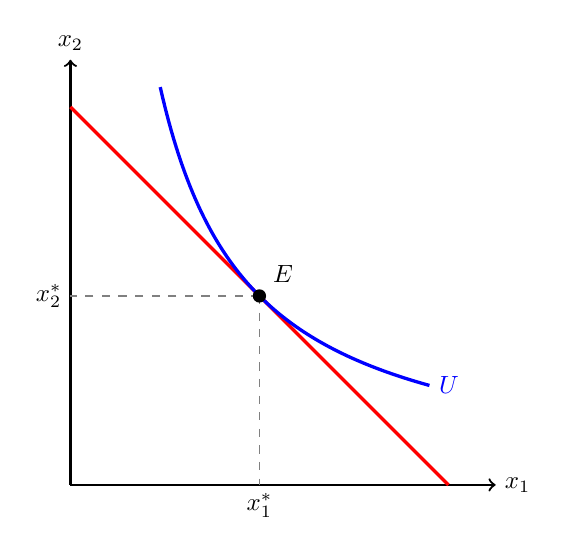
\begin{tikzpicture}[scale=1.2, every node/.style={scale=0.9}]
					% 坐标轴
					\draw[->, thick] (0,0) -- (4.5,0) node[right] {$x_1$};
					\draw[->, thick] (0,0) -- (0,4.5) node[above] {$x_2$};
					
					% 预算线: x1 + x2 = 4 (斜率为 -1)
					\draw[very thick, red] (0,4) -- (4,0);;
					
					% 无差异曲线: 使用 y = 4/x 确保在 (2,2) 处完美相切
					% domain 控制绘制范围，samples 保证曲线圆滑
					\draw[very thick, blue, domain=0.95:3.8, samples=100] 
					plot (\x, {4/\x}) node[right] {$U$};
					
					% 均衡点辅助虚线
					\draw[dashed, gray] (2,2) -- (2,0) node[below, black] {$x_1^*$};
					\draw[dashed, gray] (2,2) -- (0,2) node[left, black] {$x_2^*$};
					
					% 切点标注与防止遮挡
					\fill[black] (2,2) circle (2pt);
					\node[above right, xshift=2pt, yshift=2pt] at (2,2) {$E$};
					
				\end{tikzpicture}
			\end{center}
			\newpage
			\item \textbf{描述与互为完全替代品的两种商品相对应的无差异曲线。假如为完全互补品又怎么样呢？}
			
			\textbf{答：}
			
			1. 完全替代品：两种商品能够按照固定比例相互替代，其无差异曲线是一组相互平行、向右下方倾斜的直线，边际替代率恒定不变。
			
			2. 完全互补品：两种商品必须按照固定搭配比例一同消费，无法单独替代，对应的无差异曲线呈现直角弯折（L型）形态，直角的拐点代表最优搭配的消费组合。
			
			\begin{center}
				\begin{tikzpicture}[scale=1.1, every node/.style={scale=0.9}]
					% --- 左图：完全替代品 ---
					\begin{scope}[xshift=0cm]
						\draw[->] (0,0) -- (3.5,0) node[right] {\text{商品 }$1$};
						\draw[->] (0,0) -- (0,3.5) node[above] {\text{商品 }$2$};
						
						% 修改了节点位置：通过 anchor 和适度偏移，将 U1, U2, U3 整体向上提，避免与横轴重叠
						\draw[thick, blue] (0,2.5) -- (2.5,0) node[anchor=south west, xshift=-9pt, yshift=2pt] {$U_3$};
						\draw[thick, blue] (0,1.8) -- (1.8,0) node[anchor=south west, xshift=-9pt, yshift=2pt] {$U_2$};
						\draw[thick, blue] (0,1.1) -- (1.1,0) node[anchor=south west, xshift=-9pt, yshift=2pt] {$U_1$};
						
						\node[below] at (1.75,-0.5) {(a) 完全替代品};
					\end{scope}
					
					% --- 右图：完全互补品 ---
					\begin{scope}[xshift=6cm]
						\draw[->] (0,0) -- (3.5,0) node[right] {\text{商品 }$1$};
						\draw[->] (0,0) -- (0,3.5) node[above] {\text{商品 }$2$};
						
						% L型无差异曲线
						\draw[thick, red] (1.0,3.0) -- (1.0,1.0) -- (3.0,1.0) node[right] {$U_1$};
						\draw[thick, red] (1.7,3.0) -- (1.7,1.7) -- (3.0,1.7) node[right] {$U_2$};
						\draw[thick, red] (2.4,3.0) -- (2.4,2.4) -- (3.0,2.4) node[right] {$U_3$};
						
						% 拐点射线（固定搭配比例）
						\draw[dashed, gray] (0,0) -- (3.0,3.0);
						
						\node[below] at (1.75,-0.5) {(b) 完全互补品};
					\end{scope}
				\end{tikzpicture}
			\end{center}
			
			\item \textbf{序数效用和基数效用的区别是什么？解释对消费者选择进行排序时为什么不需要基数效用的假定。}
			
			\textbf{答：}
			
			序数效用与基数效用的核心区别在于对“效用是否可以量化”的认知不同。
			
			基数效用论认为，效用是可以具体量化和精确度量的。就像长度有“米”、重量有“千克”一样，效用也可以用明确的绝对数值（如 10 个效用单位）来表示满足程度的高低。这种理论主要采用边际效用分析法来研究消费者行为。
			
			序数效用论则认为，效用只是一种主观心理感受，无法精准量化。在现实中，消费者只需要也能对不同商品组合的偏好程度进行相对高低的“排序”（比如第一、第二、第三），而不需要明确知道具体高出多少数值。该理论主要使用无差异曲线与预算线作为核心分析工具。
			
			在对消费者选择进行分析时，之所以不需要基数效用的假定，是因为基数效用依赖的主观数值度量在现实中缺乏统一且客观的衡量标准，理论显得不够严谨。只要明确消费者对不同商品组合的偏好次序（即能判断出“更喜欢 A 还是 B”，或者“两者无差异”），就可以画出完整的无差异曲线。结合预算约束，这已经足够推导出消费者的最优选择和需求规律。由于序数效用足以完成全部的逻辑推导，且更加贴合人们现实的决策直觉，因此经济学就不再需要引入复杂且难以证伪的基数效用假定了。
			
			\newpage
			\item \textbf{画一条预算线，然后再画一条无差异曲线来说明与两种商品相对应的满足最大化选择。利用图形回答下述问题：\\ a. 假定其中一种商品实施配给。解释为什么消费者的境况可能变坏。\\ b. 假定其中一种商品被固定在当前市场价格以下水平，因此消费者不能想买多少就买多少。你能判断消费者的境况是变好了还是变坏了吗？}
			
			\textbf{答：}
			
			在没有任何限制的市场中，消费者通过寻找无差异曲线和预算线的切点来实现效用最大化。
			
			a.配给对福利的影响：当政府设置配给额度$\bar{x}_1$时，预算线会从配给点处垂直弯折，如果消费者原先的最优消费量超出了该额度，那么其可以得到的消费组合集将成为原来那个额度下的一个真子集。这样消费者不能停留在原来的最优无差异曲线上面，而是必须向左下方移动去寻找新的次优均衡点。由于新的最优决策点意味着更低水平的无差异曲线使消费者的总体效用降低，因此他们变坏。
			
			b.最高限价与短缺的不确定性：最高限价使商品的价格下降，预算线也随之变得更加平缓，增加了消费者的潜在购买力，但由于低廉的供给造成了供给短缺的存在，结果就是消费者的实际消费量被限定在供给配额$x_s$内。如果限价带来的收入足够弥补由购买限制导致的效用损失，那么消费者的福利水平可能提升；相反如果供给限制非常严厉，消费者的最好消费将极易偏离自己的喜好轨迹，使自身境况甚至比限价前还糟糕。所以限价政策对消费者产生的影响依赖于供给短缺程度的大小。
			
			\begin{center}
				\begin{tikzpicture}[scale=0.8, every node/.style={scale=0.75}]
					% --- 图 (a): 商品配给 (境况变坏) ---
					\begin{scope}[xshift=0cm]
						\draw[->] (0,0) -- (4,0) node[right] {$x_1$};
						\draw[->] (0,0) -- (0,4) node[above] {$x_2$};
						% 原预算线: x + y = 3
						\draw[dashed, gray] (0,3) -- (3,0);
						% 原均衡点: xy = 2.25 (1.5, 1.5)
						\draw[thick, blue!40, domain=0.8:2.8] plot (\x, {2.25/\x}) node[above] {$U_0$};
						\fill (1.5,1.5) circle (2pt) node[above right] {$E_0$};
						% 现在的预算线：配给 x=1。转折点 (1, 2)
						\draw[very thick, red] (0,3) -- (1,2); 
						\draw[very thick, red] (1,2) -- (1,0);   
						\draw[dashed, red] (1,2) -- (3,0);   
						\node[red, below] at (1,0) {$\bar{x}_1$};
						% 新均衡点: 落在垂直线上 (1, 2)。U = xy = 2
						\draw[thick, blue, domain=0.6:2.8] plot (\x, {2/\x}) node[right] {$U_R$};
						\fill (1,2) circle (2pt) node[above right] {$E_R$};
						\node[below] at (2,-0.8) {(a) 配给};
					\end{scope}
					
					% --- 图 (b): 最高限价 (境况变好) ---
					\begin{scope}[xshift=5.2cm]
						\draw[->] (0,0) -- (4,0) node[right] {$x_1$};
						\draw[->] (0,0) -- (0,4) node[above] {$x_2$};
						% 原预算线: x + y = 2.5。均衡 xy = 1.5625
						\draw[gray] (0,2.5) -- (2.5,0);
						\draw[thick, blue!30] plot[domain=0.7:2.4] (\x, {1.56/\x});
						\fill (1.25,1.25) circle (1.8pt) node[below left] {$E_0$};
						% 限价后预算线: 0.5x + y = 2.5。x_s = 2 时, y = 1.5。转折点 (2, 1.5)
						\draw[very thick, red] (0,2.5) -- (2,1.5); 
						\draw[very thick, red] (2,1.5) -- (2,0);   
						\draw[dashed, red] (2,1.5) -- (5,0);  
						\node[red, below] at (2,0) {$x_s$};
						% 新均衡点: (2, 1.5)。U = xy = 3
						\fill (2,1.5) circle (2pt) node[above right] {$E_1$};
						\draw[thick, blue] plot[domain=1.1:3.2] (\x, {3/\x}) node[right] {$U_1$};
						\node[below] at (2,-0.8) {(b) 限价：福利改善};
					\end{scope}
					
					% --- 图 (c): 最高限价 (境况变差) ---
					\begin{scope}[xshift=10.4cm]
						\draw[->] (0,0) -- (4,0) node[right] {$x_1$};
						\draw[->] (0,0) -- (0,4) node[above] {$x_2$};
						% 原预算线同上
						\draw[gray] (0,2.5) -- (2.5,0);
						\draw[thick, blue!30] plot[domain=0.7:2.9] (\x, {1.56/\x});
						\fill (1.25,1.25) circle (1.8pt) node[above right,yshift=-5pt] {$E_0$};
						% 限价同上。但供给极度匮乏: x_s = 0.5。转折点 (0.5, 2.25)
						\draw[very thick, red] (0,2.5) -- (0.5,2.25); 
						\draw[very thick, red] (0.5,2.25) -- (0.5,0); 
						\draw[dashed, red] (0.5,2.25) -- (5,0);   
						\node[red, below] at (0.5,0) {$x_s$};
						% 新均衡点: (0.5, 2.25)。U = xy = 1.125
						\fill (0.5,2.25) circle (2pt) node[above right] {$E_2$};
						\draw[thick, blue, domain=0.3:2.9] plot (\x, {1.12/\x}) node[right] {$U_2$};
						\node[below] at (2,-0.8) {(c) 限价：福利受损};
					\end{scope}
				\end{tikzpicture}
			\end{center}
			
			\newpage
			\item \textbf{描述边际相等原则。解释一下，为什么如果一种或两种商品的消费具有递增的边际效用，这一原则可能并不成立。}
			
			\textbf{答：}
			
			1. 边际相等原则：这是消费者效用最大化的核心准则。它指的是在收入与商品价格既定的条件下，消费者最优消费组合必须满足：两种商品的边际替代率等于商品的价格之比，这也等价于花费在每一种商品上的最后一单位货币所获得的边际效用彼此相等。其数学表达式如下：

				$$MRS_{12} = \frac{P_1}{P_2} = \frac{MU_1}{MU_2} \implies \frac{MU_1}{P_1} = \frac{MU_2}{P_2} = \lambda$$

			其中 $\lambda$ 为货币的边际效用。在此条件下，消费者无法通过调整消费组合进一步提升总效用，从而达到均衡状态。
			
			2. 边际效用递增时原则失效的原因：常规商品满足边际效用递减规律，存在内点最优解，因此边际相等原则成立。但如果商品存在边际效用递增的特征（例如成瘾性物品），消费者增加消费量时，额外获得的边际效用会持续上升。此时，消费者会产生不断加大单一商品消费的动机，其最优选择通常为角点解（即将其全部收入集中用于购买边际效用递增的商品），不再遵循将消费均等分配的等边际规则。因此，在这种情况下，边际相等原则不再成立。
			
			\begin{center}
				\begin{tikzpicture}[scale=1.2, every node/.style={scale=0.9}]
					% --- 左图：正常商品 (凸向原点，内点解) ---
					\begin{scope}[xshift=0cm]
						% 坐标轴
						\draw[->, thick] (0,0) -- (4,0) node[right] {商品 $1$};
						\draw[->, thick] (0,0) -- (0,4) node[above] {商品 $2$};
						
						% 预算线: x + y = 3
						\draw[thick, red] (0,3) -- (3,0);;
						
						% 无差异曲线 (凸向原点) 
						\draw[very thick, blue, domain=0.75:3.4, samples=100] 
						plot (\x, {2.25/\x}) node[right] {$U_1$};
						
						% 均衡点标注
						\fill (1.5,1.5) circle (2pt);
						\node[above right, xshift=2pt] at (1.5,1.5) {$E$};
						
						\node[below] at (1.75,-0.6) {(a) 边际效用递减};
					\end{scope}
					
					% --- 右图：成瘾商品 (凹向原点，角点解) ---
					\begin{scope}[xshift=6cm]
						% 坐标轴
						\draw[->, thick] (0,0) -- (4,0) node[right] {普通商品};
						\draw[->, thick] (0,0) -- (0,4) node[above] {成瘾商品};
						
						% 预算线: x + y = 3
						\draw[thick, red] (0,3) -- (3,0);
						
						% 较低的无差异曲线 (切点效用极小)
						% 使用 arc 画完美圆弧：半径 sqrt(4.5) ≈ 2.1213，确保严丝合缝
						\draw[thick, blue!40] (2.1213,0) arc (0:90:2.1213);
						\node[blue!40] at (2.3, 0.4) {$U_1$};
						
						\fill[gray] (1.5,1.5) circle (1.5pt);
						\node[above right, xshift=0pt, yshift=-2pt, gray] at (1.5,1.5) { $E'$ };
						
						% 较高的无差异曲线 (角点效用极大)
						% 使用 arc 画完美圆弧：半径 3，完美连接 (3,0) 和 (0,3)
						\draw[very thick, blue] (3,0) arc (0:90:3);
						\node[blue] at (3.3, 0.4) {$U_2$};
						
						% 角点解标注 (全部收入购买成瘾商品)
						\fill[red] (0,3) circle (2.5pt);
						\node[right, xshift=1pt, yshift=6pt] at (0,3) {$E^*$ （最优点）};
						
						\node[below] at (1.75,-0.6) {(b) 边际效用递增};
					\end{scope}
				\end{tikzpicture}
			\end{center}
			\newpage
			\item \textbf{在过去20年中计算机的价格已经大幅下跌。请用这一价格下跌的情况解释为什么消费者价格指数可能在很大程度上高估了那些密集使用计算机的人的生活成本指数。}
			
			\textbf{答：}
			
			消费者价格指数（CPI）本质上是一种拉氏价格指数，它采用固定基期的商品消费篮子来计算价格变动。这种计算方式存在两类系统性偏误，导致其在面对计算机价格大幅下跌时，会高估密集使用计算机人群的真实生活成本：
			
			1. 替代偏误：拉氏指数固定了基期的消费篮子，没有考虑消费者的替代行为。在计算机价格大幅下跌后，消费者理性的选择是增加计算机的购买量，以替代其他价格相对更高的商品。然而，CPI 仍然以基期的固定权重进行计算，无法反映消费者通过调整消费结构所带来的成本节约，因此高估了实际的生活成本。
			
			2. 质量变化偏误：CPI 未能充分核算商品质量的提升。在过去20年中，计算机价格下跌的同时，其性能、算力和功能等质量指标出现了飞跃式的提升。CPI 往往将这种质量提升带来的巨大效用增益，误判为单纯的商品价格下降，从而低估了消费者的真实购买力，这也进一步导致了对生活成本的高估。
			
			\item \textbf{解释为什么帕氏指数通常会低估理想生活成本指数。}
			
			\textbf{答：}
			
			1. 核心定义：
			帕氏指数是以当期消费组合为权重的价格指数，即用当期价格购买当期组合的成本，与基期价格购买当期组合的成本之比。其核心计算公式如下：

				$$\text{帕氏指数} = \frac{\sum P_t Q_t}{\sum P_0 Q_t}$$

			相对而言，理想生活成本指数是指以当期价格实现基期效用水平所需的最小成本，与基期实现该效用的成本之比。
			
			2. 低估原因：
			帕氏指数采用当期消费组合 $Q_t$ 作为权重，而 $Q_t$ 是消费者在当期价格下，已经根据价格变动完成了消费替代（即减少购买涨价商品、增加购买降价商品）之后的最终结果。这种替代行为自然压低了涨价商品在总消费中的权重，使得帕氏指数计算出的成本变化，低于消费者“维持基期效用不变”所需要面临的真实成本变化。因此，帕氏指数通常会系统性地低估理想生活成本指数。
		\end{enumerate}
		\newpage
	\section{练习题}
		\begin{enumerate}[label=\textbf{\arabic*.}, leftmargin=*]		
			\item \textbf{在本章中，对于不同商品的消费者偏好在分析中没有发生变化。不过在有些情况下，消费时偏好的确会变化。讨论一下，就消费下述这两种商品而言，偏好为什么以及怎样在一段时间后可能会变化。\\ a. 卷烟；\\b. 在一家有特色菜肴的餐厅里初次用餐。}
			
			\textbf{答：}
			
			a. 卷烟为成瘾性商品，消费后尼古丁依赖增强，边际效用递增，对卷烟的偏好随消费次数增加而持续增强。
			
			b. 特色餐厅初次用餐为体验品，偏好随体验结果变化：体验良好则偏好正向增强，体验不佳则偏好减弱甚至消失。
			
			\begin{center}
				\begin{tikzpicture}[scale=0.8, every node/.style={scale=0.8}]
					% --- 图 (a)：卷烟 (偏好增强) ---
					\begin{scope}[xshift=0cm]
						\draw[->, thick] (0,0) -- (3.5,0) node[right] {卷烟};
						\draw[->, thick] (0,0) -- (0,3.5) node[above] {其他商品};
						% 初始 U1
						\draw[thick, gray] (0.5,2.5) -- (2.5,0.5);
						\node[gray, right, fill=white, inner sep=1pt] at (2.5,0.5) {$U_1$};
						% 变动后 U2 (更陡)
						\draw[thick, red, dashed] (0.5,3.0) -- (2.2,0.3);
						\node[red, right, yshift=5pt, fill=white, inner sep=1pt] at (1.5,0.3) {$U_2$};
						\node[below] at (1.75,-0.6) {\textbf{(a) 卷烟：偏好增强}};
					\end{scope}
					
					% --- 图 (b)：餐厅 (体验良好 -> 偏好增强) ---
					\begin{scope}[xshift=5.8cm]
						\draw[->, thick] (0,0) -- (3.5,0) node[right] {餐厅};
						\draw[->, thick] (0,0) -- (0,3.5) node[above] {其他};
						% 初始 U1
						\draw[thick, gray] (0.5,2.5) -- (2.5,0.5);
						\node[gray, right, fill=white, inner sep=1pt] at (2.5,0.5) {$U_1$};
						% 变动后 U2 (斜率变陡，标注上移)
						\draw[thick, blue, dashed] (0.5,3.2) -- (2.0,0.8);
						\node[blue, right, yshift=8pt, fill=white, inner sep=1pt] at (1.7,1.4) {$U_2$};
						\node[below] at (1.75,-0.6) {\textbf{(b) 餐厅：体验良好}};
					\end{scope}
					
					% --- 图 (c)：餐厅 (体验不佳 -> 偏好减弱) ---
					\begin{scope}[xshift=11.6cm]
						\draw[->, thick] (0,0) -- (3.5,0) node[right] {餐厅};
						\draw[->, thick] (0,0) -- (0,3.5) node[above] {其他};
						% 初始 U1
						\draw[thick, gray] (0.5,2.5) -- (2.5,0.5);
						\node[gray, right, fill=white, inner sep=1pt] at (2,1.5) {$U_1$};
						% 变动后 U2 (斜率变平缓，标注上移)
						\draw[thick, red, dashed] (0.5,1.8) -- (3.2,0.2);
						\node[red, right, yshift=8pt, fill=white, inner sep=1pt] at (3.2,0.2) {$U_2$};
						\node[below] at (1.75,-0.6) {\textbf{(c) 餐厅：体验不佳}};
					\end{scope}
				\end{tikzpicture}
			\end{center}
		
			\item \textbf{画出下述两种商品个人偏好的无差异曲线：汉堡包和软饮料。指出个人满足（或效用）增加的方向。\\ a. 乔的无差异曲线为凸的，汉堡包和软饮料都不喜欢。\\ b. 简喜欢汉堡包，但不喜欢软饮料。如果服务员给她一份软饮料，她会不喝倒掉。\\ c. 鲍勃喜欢汉堡包，但不喜欢软饮料。但是如果服务员给他一份软饮料，为了礼貌起见他会喝掉。\\ d. 莫利喜欢汉堡包和软饮料，但坚持精确地按照两个汉堡包搭配一份软饮料来吃。\\ e. 比尔喜欢汉堡包，但对软饮料无所谓喜欢或不喜欢。\\ f. 玛丽从额外一份汉堡包中获得的满足是从额外一份软饮料中所获得满足的两倍。}
			
			\textbf{答：}
			
			a. 两者均为厌物品，无差异曲线凸向原点，效用向原点方向（左下方）增加。
			
			b. 软饮料为厌物品，汉堡包为喜好品。无差异曲线向右上方倾斜，效用随汉堡增加、软饮料减少（向右下方）而增加。
			
			c. 同 b，软饮料对其依然产生负效用（需要强迫自己喝掉），无差异曲线向右上方倾斜，效用向右下方增加。
			
			d. 汉堡与软饮料为完全互补品，无差异曲线为直角形，直角拐点在 $H = 2S$ 射线上，效用向右上方增加。
			
			e. 软饮料为中性商品，无差异曲线为垂直于汉堡包轴的直线（若汉堡在横轴则为垂直线，若在纵轴则为水平线。本图示将其置于纵轴则为水平线，效用向右方增加）。
			
			f. 汉堡与软饮料为完全替代品，无差异曲线为斜率恒定的直线，斜率绝对值为 $1/2$（横轴为汉堡时），效用向右上方增加。
			
			\begin{center}
				\begin{tikzpicture}[scale=0.8, every node/.style={scale=0.85}]
					% ==================== 第一行 ====================
					
					% --- a. 乔：双厌物品 ---
					\begin{scope}[xshift=0cm, yshift=0cm]
						\draw[->, thick] (0,0) -- (3.5,0) node[right] {汉堡};
						\draw[->, thick] (0,0) -- (0,3.5) node[above] {软饮};
						
						% U1 (外侧，效用较低)
						\draw[thick, blue, domain=0.8:2.8, samples=50] plot (\x, {2.25/\x}) node[right] {$U_1$};
						% U2 (内侧，效用较高，靠近原点)
						\draw[thick, blue, domain=0.4:2.5, samples=50] plot (\x, {1/\x}) node[below,xshift=8pt,yshift=5pt] {$U_2$};
						
						% 效用增加箭头 (严格在两线之间，向左下方)
						\draw[->, red, thick] (1.3, 1.3) -- (1.1, 1.1);
						
						\node[below] at (1.75,-0.6) {(a) 乔：都讨厌};
					\end{scope}
					
					% --- b. 简：厌软饮 ---
					\begin{scope}[xshift=5.2cm, yshift=0cm]
						\draw[->, thick] (0,0) -- (3.5,0) node[right] {汉堡};
						\draw[->, thick] (0,0) -- (0,3.5) node[above] {软饮};
						
						% U1 (左上方，效用较低)
						\draw[thick, blue] (0.5, 1.5) -- (2.0, 3.0) node[right] {$U_1$};
						% U2 (右下方，效用较高)
						\draw[thick, blue] (1.5, 0.5) -- (3.0, 2.0) node[right] {$U_2$};
						
						% 效用增加箭头 (严格在两线之间，向右下方)
						\draw[->, red, thick] (1.2, 1.9) -- (1.9, 1.2);
						
						\node[below] at (1.75,-0.6) {(b) 简：讨厌软饮};
					\end{scope}
					
					% --- c. 鲍勃：厌软饮 ---
					\begin{scope}[xshift=10.4cm, yshift=0cm]
						\draw[->, thick] (0,0) -- (3.5,0) node[right] {汉堡};
						\draw[->, thick] (0,0) -- (0,3.5) node[above] {软饮};
						
						% U1 (左上方，效用较低)
						\draw[thick, blue] (0.5, 1.5) -- (2.0, 3.0) node[right] {$U_1$};
						% U2 (右下方，效用较高)
						\draw[thick, blue] (1.5, 0.5) -- (3.0, 2.0) node[right] {$U_2$};
						
						% 效用增加箭头 (严格在两线之间，向右下方)
						\draw[->, red, thick] (1.2, 1.9) -- (1.9, 1.2);
						
						\node[below] at (1.75,-0.6) {(c) 鲍勃：讨厌软饮};
					\end{scope}
					
					% ==================== 第二行 ====================
					% 增大 yshift 的负值（从 -4.5cm 改为 -6.0cm），彻底避免与第一行重叠
					
					% --- d. 莫利：完全互补 ---
					\begin{scope}[xshift=0cm, yshift=-6.0cm]
						\draw[->, thick] (0,0) -- (3.5,0) node[right] {汉堡};
						\draw[->, thick] (0,0) -- (0,3.5) node[above] {软饮};
						
						% 比例射线
						\draw[dashed, gray] (0,0) -- (2.5,1.25);
						
						% U1 (靠近原点)
						\draw[thick, blue] (0.8, 2.5) -- (0.8, 0.4) -- (2.5, 0.4) node[right] {$U_1$};
						% U2 (远离原点)
						\draw[thick, blue] (1.6, 2.5) -- (1.6, 0.8) -- (2.5, 0.8) node[right] {$U_2$};
						
						% 效用增加箭头 (沿比例射线向右上方)
						\draw[->, red, thick] (1.1, 0.55) -- (1.4, 0.7) ;
						
						\node[below] at (1.75,-0.6) {(d) 莫利：完全互补};
					\end{scope}
					
					% --- e. 比尔：中性商品 ---
					\begin{scope}[xshift=5.2cm, yshift=-6.0cm]
						\draw[->, thick] (0,0) -- (3.5,0) node[right] {汉堡};
						\draw[->, thick] (0,0) -- (0,3.5) node[above] {软饮};
						
						% U1 (靠左)
						\draw[thick, blue] (1.0, 0) -- (1.0, 2.8) node[above] {$U_1$};
						% U2 (靠右)
						\draw[thick, blue] (2.0, 0) -- (2.0, 2.8) node[above] {$U_2$};
						
						% 效用增加箭头 (向右方)
						\draw[->, red, thick] (1.2, 1.5) -- (1.8, 1.5) ;
						
						\node[below] at (1.75,-0.6) {(e) 比尔：中性商品};
					\end{scope}
					
					% --- f. 玛丽：完全替代 ---
					\begin{scope}[xshift=10.4cm, yshift=-6.0cm]
						\draw[->, thick] (0,0) -- (3.5,0) node[right] {汉堡};
						\draw[->, thick] (0,0) -- (0,3.5) node[above] {软饮};
						
						% U1 (靠近原点，斜率为 -2)
						\draw[thick, blue] (0, 2.0) -- (2.0, 0) node[right,xshift=-2pt,yshift=6pt] {$U_1$};
						% U2 (远离原点，斜率为 -2)
						\draw[thick, blue] (0, 3.0) -- (3, 0) node[right,xshift=-4pt,yshift=9pt] {$U_2$};
						
						% 效用增加箭头 (向右上方)
						\draw[->, red, thick] (1, 1) -- (1.45, 1.45);		
						\node[below] at (1.75,-0.6) {(f) 玛丽：完全替代};
					\end{scope}
				\end{tikzpicture}
			\end{center}
			
			\item \textbf{假如简目前愿意以4张电影票来换取1张篮球赛门票，那么与电影相比，她肯定更喜欢篮球。这一说法是对还是错？请解释。}
			
			\textbf{答：}
			
			该说法错误。
			
			边际替代率（$MRS$）反映的仅仅是消费者在特定消费组合下的边际意愿：
				$$MRS = \frac{MU_{\text{篮球}}}{MU_{\text{电影}}} = 4$$
			这仅说明在现有持有量下，额外 $1$ 张篮球赛门票带来的边际效用是 $1$ 张电影票的 $4$ 倍，不能等同于她整体更喜欢篮球。根据边际效用递减规律，如果简当前手里有大量电影票而几乎没有篮球票，电影票的边际效用会被拉低，自然愿意用多张电影票换 $1$ 张篮球票，这种高边际替代率是由初始资源禀赋决定的，而非绝对偏好排序。此外，她愿意换票也不一定是因为喜欢篮球运动本身，可能是为了陪同亲友、观看赛场偶像等衍生需求，这些因素同样会提高篮球票对她的边际效用。因此，仅凭边际交换意愿无法判定她与电影相比更喜欢篮球，题干说法不成立。
			
			\begin{center}
				\begin{tikzpicture}[scale=1.2, every node/.style={scale=0.9}]
					% 坐标轴
					\draw[->, thick] (0,0) -- (4.5,0) node[right] {电影票};
					\draw[->, thick] (0,0) -- (0,4.5) node[above] {篮球门票};
					
					% 无差异曲线 (y = 2/x)
					\draw[very thick, blue, domain=0.55:4, samples=100] 
					plot (\x, {2/\x}) node[right, fill=white, inner sep=1pt] {$U$};
					
					% 切线标注与延长 (在 x=3 处，斜率约为 -0.22)
					% 为了视觉平衡，绘制一段较长的切线
					\draw[dashed, red, thick] (1.5, 1.0) -- (4.2, 0.4);
					
					% 切点 A 及其标注
					\fill[black] (3.0, 0.67) circle (2pt);
					\node[above right, fill=white, inner sep=1pt, yshift=3pt] at (3.0, 0.67) {$A$ (此处 $MRS=4$)};
					
	
					
				\end{tikzpicture}
			\end{center}
			
			\item \textbf{加内勒和布赖恩每个人计划花费20000美元在汽车的款式和油耗这两个性能上。他们可以选择款式，也可以选择油耗，或者是两者的组合。加内勒对款式无所谓，但是希望油耗尽可能地低。布赖恩对两者的喜欢程度相同，想在每样性能上花费相同数额的钱。利用无差异曲线和预算线，说明两人各将做怎样的选择。}
			
			\textbf{答：}
			
			加内勒：款式对她而言是中性商品，她仅偏好低油耗（即高燃油经济性）。因此，她的无差异曲线是水平线。她的最优选择是角点解，即将全部 $20000$ 美元预算用于购买高燃油经济性，而在款式上的支出为 $0$。
			
			布赖恩：款式与燃油经济性对他而言是完全替代品，且偏好程度等同。如果两者价格一致，他的最优选择是内点解，比如在款式和燃油经济性上各花费 $10000$ 美元。
			
			\begin{center}
				\begin{tikzpicture}[scale=1.1, every node/.style={scale=0.9}]
					% --- 左图：加内勒 (款式中性，偏好低油耗) ---
					\begin{scope}[xshift=1.2cm]
						\draw[->, thick] (0,0) -- (3.5,0) node[right] {款式};
						\draw[->, thick] (0,0) -- (0,3.5) node[above] {燃油经济性};
						
						% 预算线
						\draw[very thick, black] (0,3) -- (3,0);
						
						% 无差异曲线族 (水平线)
						\draw[thick, blue] (0,1.8) -- (3.2,1.8) node[right] {$U_1$};
						\draw[thick, blue] (0,3) -- (3.2,3) node[right] {$U_2$};
						
						% 效用增加箭头 (添加文字说明，避免空箭头)
						\draw[->, red, thick] (2.2, 2.0) -- (2.2, 2.8);
						
						% 均衡点标注
						\fill[red] (0,3) circle (2.5pt);
						\node[left, xshift=-4pt, fill=white, inner sep=1pt] at (0,3) {最优解 (角点)};
						
						\node[below] at (1.75,-0.7) {\textbf{(a) 加内勒：单方面偏好}};
					\end{scope}
					
					% --- 右图：布赖恩 (完全替代且均等消费) ---
					\begin{scope}[xshift=8cm]
						\draw[->, thick] (0,0) -- (4,0) node[right] {款式};
						\draw[->, thick] (0,0) -- (0,4) node[above] {燃油经济性};
						
						% 预算线
						\draw[very thick, black] (0,3) -- (3,0);
						
						% 支出相等线 (y=x)
						\draw[dashed, gray!80, thick] (0,0) -- (3.2,3.2);
						
						% 无差异曲线 U1
						\draw[thick, blue] (0,1.5) -- (1.5,0) node[right, font=\footnotesize, fill=white,yshift=9pt,xshift=-1pt] {$U_1$};
						
						% 最优无差异曲线 U2 (与预算线重合)
						\draw[thick, blue] (0,3) -- (3,0);
						\node[blue, above right, fill=white, inner sep=1pt] at (2.2,0.9) {$U_2$ （和预算线重合）};
						
						% 效用增加箭头 (添加文字说明)
						\draw[->, red, thick] (0.8, 0.8) -- (1.2, 1.2);
						
						% 投影虚线
						\draw[dashed, gray] (1.5,0) node[below, black] {\small 10000} -- (1.5,1.5) -- (0,1.5) node[left, black] {\small 10000};
						
						% 均衡点及文字标注 (修复点：补全了 {} 及其中的内容)
						\fill[red] (1.5,1.5) circle (2.5pt);
						
						\node[below] at (1.75,-0.7) {\textbf{(b) 布赖恩：均衡偏好}};
					\end{scope}
				\end{tikzpicture}
			\end{center}
			
			\item \textbf{假如布里奇特和艾玲的收入花在两种商品上——食品（$F$）和衣服（$C$）。布里奇特的偏好效用函数 $U(F, C) = 10FC$ 表示，而艾玲的偏好用效用函数 $U(F, C) = 0.20F^2C^2$ 表示。\\ a. 以食品为横轴，以衣服为纵轴，在图上找到能给予布里奇特与组合（10，5）相同效用水平的点集。在另一幅图上为艾玲找到相同的点集。\\ b. 在同样两幅图中，分别找出能给予布里奇特和艾玲与组合（15，8）一样效用水平的点集。\\ c. 你认为布里奇特和艾玲的偏好相同吗？请解释。}
			
			\textbf{答：}
			
			a. 对于组合 $(10, 5)$：
	
				布里奇特的效用为 $U_B = 10 \times 10 \times 5 = 500$，无差异曲线方程为 $FC = 50$。\\
				艾玲的效用为 $U_E = 0.20 \times 10^2 \times 5^2 = 500$，无差异曲线方程同样为 $FC = 50$。
	
			二者在此组合下的点集完全重合。
			
			b. 对于组合 $(15, 8)$：
	
				布里奇特的效用为 $U_B = 10 \times 15 \times 8 = 1200$，无差异曲线方程为 $FC = 120$。\\
				艾玲的效用为 $U_E = 0.20 \times 15^2 \times 8^2 = 2880$，无差异曲线方程化简后同样为 $FC = 120$。
	
			二者在此组合下的点集依然完全重合。
			\newpage
			c. 布里奇特和艾玲的偏好完全相同。
	
				$$U_E = 0.20(FC)^2 = 0.20 \left(\frac{U_B}{10}\right)^2 = 0.002 U_B^2$$
	
			由于 $U_B > 0$，艾玲的效用函数是布里奇特效用函数的严格正单调变换。序数效用论认为，效用函数的绝对数值并不重要，只要单调性一致，它们所反映的商品组合的排序偏好以及无差异曲线族就是完全相同的。
			
			\begin{center}
				\begin{tikzpicture}[scale=1.1, every node/.style={scale=0.9}]
					% --- 左图：组合 (10, 5) ---
					\begin{scope}[xshift=0cm]
						\draw[->, thick] (0,0) -- (4,0) node[right] {\text{食品 }$F$};
						\draw[->, thick] (0,0) -- (0,4) node[above] {\text{衣服 }$C$};
						
						\draw[very thick, blue, domain=0.4:3.5, samples=100] plot (\x, {1.5/\x});
						
						\fill (1.5,1.0) circle (2pt);
						\node[above right] at (1.5,1.0) {$(10,5)$};
						\node[below] at (2,-0.5) {\text{点集 }$FC=50$};
					\end{scope}
					
					% --- 右图：组合 (15, 8) ---
					\begin{scope}[xshift=6cm]
						\draw[->, thick] (0,0) -- (4,0) node[right] {\text{食品 }$F$};
						\draw[->, thick] (0,0) -- (0,4) node[above] {\text{衣服 }$C$};
						
						\draw[very thick, red, domain=0.8:3.8, samples=100] plot (\x, {3.0/\x});
						
						\fill (2.0,1.5) circle (2pt);
						\node[above right] at (2.0,1.5) {$(15,8)$};
						\node[below] at (2,-0.5) {\text{点集 }$FC=120$};
					\end{scope}
				\end{tikzpicture}
			\end{center}
			
			\item \textbf{假设琼斯和史密斯已决定每年花1000美元在曲棍球赛或摇滚音乐会这两种形式的娱乐上。他们都喜欢这两种商品，将会选择消费正数量的这两种商品。但对这两种形式的娱乐，琼斯和史密斯在他们的偏好方面分歧很大，琼斯更偏好曲棍球赛，而史密斯则更偏好摇滚音乐会。\\ a. 为琼斯画一组无差异曲线，为史密斯画第二组曲线。\\ b. 运用边际替代率概念解释为什么这两组曲线彼此不一样。}
			
			\textbf{答：}
			
			a. 设横轴为摇滚音乐会场次 $R$，纵轴为曲棍球赛场次 $H$。琼斯更偏好曲棍球赛，史密斯更偏好摇滚音乐会，两人的无差异曲线特征如下：
			
			\begin{center}
				\begin{tikzpicture}[scale=1.1, every node/.style={scale=0.9}]
					% --- 琼斯的无差异曲线 (偏好 H，曲线较平缓) ---
					\begin{scope}[xshift=0cm]
						\draw[->, thick] (0,0) -- (4.5,0) node[right] {\text{摇滚音乐会} $R$};
						\draw[->, thick] (0,0) -- (0,4.5) node[above] {\text{曲棍球赛} $H$};
						
						\draw[very thick, blue] plot[smooth, tension=0.8] coordinates {(0.5, 2.5) (1.5, 1.5) (3.5, 0.8)};
						\node[right, blue] at (3.5, 0.8) {$U_1$};
						
						\draw[very thick, blue] plot[smooth, tension=0.8] coordinates {(0.8, 3.5) (2.0, 2.2) (4.0, 1.4)};
						\node[right, blue] at (4.0, 1.4) {$U_2$};
						
						\node[below] at (2.25,-0.6) {\textbf{(a) 琼斯：偏好曲棍球（平缓）}};
					\end{scope}
					
					% --- 史密斯的无差异曲线 (偏好 R，曲线较陡峭) ---
					\begin{scope}[xshift=6.5cm]
						\draw[->, thick] (0,0) -- (4.5,0) node[right] {\text{摇滚音乐会} $R$};
						\draw[->, thick] (0,0) -- (0,4.5) node[above] {\text{曲棍球赛} $H$};
						
						\draw[very thick, red] plot[smooth, tension=0.8] coordinates {(0.5, 3.5) (1.0, 1.5) (2.5, 0.5)};
						\node[right, red] at (2.5, 0.5) {$U_1$};
						
						\draw[very thick, red] plot[smooth, tension=0.8] coordinates {(1.0, 4.2) (1.6, 2.4) (3.5, 1.0)};
						\node[right, red] at (3.5, 1.0) {$U_2$};
						
						\node[below] at (2.25,-0.6) {\textbf{(b) 史密斯：偏好摇滚（陡峭）}};
					\end{scope}
				\end{tikzpicture}
			\end{center}
			
			b. 边际替代率（$MRS$）的定义为消费者在保持总效用不变的前提下，为多获得一单位某种商品而愿意放弃的另一种商品的数量。在本题中：
	
				$$MRS_{RH} = - \frac{\Delta H}{\Delta R}$$
	
			此公式表示为多获得 1 单位摇滚音乐会（$R$），愿意放弃的曲棍球赛（$H$）的数量，在几何上等于无差异曲线斜率的绝对值。
	
			对于琼斯：他更偏好曲棍球赛，因此曲棍球赛对他来说边际效用很高。为了让他放弃 1 单位的曲棍球赛，需要给他大量的摇滚音乐会作为补偿。反过来说，他愿意为增加 1 单位摇滚音乐会而放弃的曲棍球赛数量极少，即 $MRS_{RH}$ 较小，导致其无差异曲线平缓。\\
			对于史密斯：他更偏好摇滚音乐会。他愿意放弃大量的曲棍球赛来换取额外的 1 单位摇滚音乐会，即 $MRS_{RH}$ 较大，导致其无差异曲线较陡峭。
	
			\item \textbf{DVD的价格（$D$）是20美元，CD的价格（$C$）是10美元。菲利普有一笔100美元的预算，可以花在这两种商品上。假设他已购买了1张DVD和1张CD。另外，他其实还想再购买3张DVD和5张CD。\\ a. 在上述价格和收入下，以横轴表示CD，画出菲利普的预算约束。\\ b. 考虑菲利普已经购买的和仍然想要购买的这两种商品，找出他可以购买的三个不同的CD与DVD的组合。假定他只能购买整数单位。}
			
			\textbf{答：}
			
			a. 菲利普的预算约束方程为：

				$$20D + 10C = 100 \implies 2D + C = 10$$
			
			\begin{center}
				\begin{tikzpicture}[scale=1.1, every node/.style={scale=0.9}]
					\draw[->, thick] (0,0) -- (6,0) node[right] {$CD$};
					\draw[->, thick] (0,0) -- (0,4) node[above] {$DVD$};
					
					% 预算线: 2D + C = 10 -> 如果 C=10(放x轴), D=5(放y轴)
					% 比例设为 1单位 = 0.5cm
					\draw[very thick, blue] (5,0) node[below, black] {$10$} -- (0,2.5) node[left, black] {$5$};
					
					% 已购买组合 (1,1) -> 坐标 (0.5, 0.5)
					\fill[black] (0.5, 0.5) circle (2pt);
					\node[right, fill=white, inner sep=1pt] at (0.8, 0.5) {\text{已购买 } $(1,1)$};

					\fill[red] (3, 2) circle (2pt);
					\node[above right, fill=white, inner sep=1pt] at (3.1, 2) {计划购买$(6,4)$};
				\end{tikzpicture}
			\end{center}
			
			b. 他想要的总购买量为 $6$ 张 CD 和 $4$ 张 DVD，总花费将达到 $6 \times 10 + 4 \times 20 = 140$ 美元，显然超出了 $100$ 美元的预算约束。由于他已经购买了 $1$ 张 DVD 和 $1$ 张 CD（花费 $30$ 美元），剩余预算为 $70$ 美元。
			满足预算且数量为整数的可行组合如下表：
			
			\begin{center}
				\begin{tabularx}{0.8\textwidth}{>{\centering\arraybackslash}X >{\centering\arraybackslash}X >{\centering\arraybackslash}X}
					\toprule
					\textbf{CD 数量 ($C$)} & \textbf{DVD 数量 ($D$)} & \textbf{总花费 (美元)} \\
					\midrule
					8 & 1 & $8 \times 10 + 1 \times 20 = 100$ \\
					6 & 2 & $6 \times 10 + 2 \times 20 = 100$ \\
					4 & 3 & $4 \times 10 + 3 \times 20 = 100$ \\
					2 & 4 & $2 \times 10 + 4 \times 20 = 100$ \\
					\bottomrule
				\end{tabularx}
			\end{center}
			
			\newpage
			\item \textbf{安妮的工作要求她每四个星期中有三个星期要外出，假定她有一个年交通预算，可以乘火车或者坐飞机。她经常去的航空公司实施了一个里程积分项目，根据她的飞行里程对机票价格打折。当她一年内的飞行里程达到25000英里之后，航空公司在该年的剩余时间里对机票减价25\%；达到50000英里之后，减价50\%。以纵轴表示火车里程数，以横轴表示飞行里程数，画出安妮的预算线。}
			
			\textbf{答：}
			
			本题的核心在于分析价格折扣如何通过改变“相对价格比”来影响预算线的斜率。
   				$$ P_{F}F+P_{T}T=M $$
				$$ k = - \frac{P_{F}}{P_{T}}$$
			
			斜率代表了安妮多飞行 1 英里的“机会成本”，即她必须放弃的火车旅行英里数。随着飞行里程增加并触发折扣，飞行价格 $P_{F}$ 会分阶段下降，导致预算线在不同的里程关口发生“转折”：
			
			1. 0 至 25000 英里阶段：飞行价格为原价 $P_F$。此时预算线最陡峭，机会成本最高。\\
			2. 25000 至 50000 英里阶段：飞行价格降为 $0.75P_F$。由于分子变小，斜率的绝对值减小，预算线在 25000 英里处发生转折并变得平缓。\\
			3. 50000 英里以上阶段：飞行价格降为 $0.5P_F$。机会成本进一步降低，预算线在 50000 英里处第二次转折，变为最平缓的一段。
			
			最终，安妮面临的是一条由三段斜率不同的线段组成的、向外凸出的折线预算线。
			\begin{center}
				\begin{tikzpicture}[scale=0.75, every node/.style={scale=0.85}]
					\draw[->, thick] (0,0) -- (8,0) node[right] {\text{飞行里程 }$F$};
					\draw[->, thick] (0,0) -- (0,5.5) node[above] {\text{火车里程 }$T$};
					
					% 设定坐标点代表不同阶段的折扣
					% 0-25000: 原价 (较陡)
					\draw[very thick, blue] (0, 5) node[left, black] {$M/P_T$} -- (2.5, 3.5);
					\node[above right, rotate=-30] at (1.25, 4.25) {\text{原价}};
					
					% 25000-50000: 75折 (变平缓)
					\draw[very thick, blue] (2.5, 3.5) -- (5.0, 2.375);
					\node[above right, rotate=-24] at (3.75, 2.9375) {\text{75折}};
					
					% >50000: 5折 (最平缓)
					\draw[very thick, blue] (5.0, 2.375) -- (8.0, 1.25);
					\node[above right, rotate=-20] at (6.5, 1.8125) {\text{5折}};
					
					% 辅助虚线与坐标轴标记
					\draw[dashed, gray] (2.5, 0) node[below, black] {$25000$} -- (2.5, 3.5);
					\draw[dashed, gray] (5.0, 0) node[below, black] {$50000$} -- (5.0, 2.375);
				\end{tikzpicture}
			\end{center}
			
			\newpage
			\item \textbf{黛布拉去电影院的时候常常会购买软饮料，她有三个选择：8盎司的饮料要价1.50美元，12盎司的饮料要价2.00美元，16盎司的饮料要价2.25美元。画出黛布拉购买饮料时面临的预算约束。（假定黛布拉处理她不需要的软饮料时无须花费成本。）}
			
			\textbf{答：}
			
			非线性定价（数量折扣）通过改变价格比来影响预算线的斜率。
			
			设纵轴为其他商品 $Y$（假设单价 $P_Y = 1$ 美元），横轴为饮料盎司数 $Q$，总预算为 $M$。预算方程和斜率可表示为：
			$$ P_{Q}Q + Y = M $$
			$$ k = - \frac{P_{Q}}{P_{Y}} = - P_{Q} $$
			
			斜率代表了黛布拉多购买 1 盎司软饮料的“机会成本”，即她必须放弃的其他商品的价值（美元）。随着购买容量的增加，软饮料的边际价格 $P_Q$ 分阶段下降，导致预算线在不同的容量关口发生“转折”：
			
			1. 0 至 8 盎司阶段：总花费 1.50 美元，边际价格为 $1.50 / 8 = 0.1875$ 美元/盎司。此时预算线最陡峭，机会成本最高。\\
			2. 8 至 12 盎司阶段：增加 4 盎司需额外花费 0.50 美元，边际价格降为 $0.50 / 4 = 0.125$ 美元/盎司。由于边际价格变小，斜率的绝对值减小，预算线在 8 盎司处发生转折并变得平缓。\\
			3. 12 至 16 盎司阶段：增加 4 盎司仅需额外花费 0.25 美元，边际价格进一步降为 $0.25 / 4 = 0.0625$ 美元/盎司。机会成本最低，预算线在 12 盎司处第二次转折，变为最平缓的一段。
			
			最终，黛布拉面临的是一条由三段斜率不同的线段组成的、向外凸出的折线预算线。
			
			\begin{center}
				\begin{tikzpicture}[scale=1.2, every node/.style={scale=0.9}]
					% 坐标轴
					\draw[->, thick] (0,0) -- (6,0) node[right] {\text{饮料盎司数 }$Q$};
					\draw[->, thick] (0,0) -- (0,4.2) node[above] {\text{其他商品 }$Y$};
					
					% 预算线绘制 (纯净版，无多余文字)
					\draw[very thick, blue] (0, 3.5) node[left, black] {$M$} -- (2, 2.0);
					\draw[very thick, blue] (2, 2.0) -- (3, 1.5);
					\draw[very thick, blue] (3, 1.5) -- (4, 1.25);
					
					% 辅助虚线与横轴标记 (容量)
					\draw[dashed, gray] (2, 2.0) -- (2, 0) node[below, black] {$8$};
					\draw[dashed, gray] (3, 1.5) -- (3, 0) node[below, black] {$12$};
					\draw[dashed, gray] (4, 1.25) -- (4, 0) node[below, black] {$16$};
					
					% 辅助虚线与纵轴标记 (剩余预算直观表达)
					\draw[dashed, gray] (2, 2.0) -- (0, 2.0) node[left, black] {$M-1.50$};
					\draw[dashed, gray] (3, 1.5) -- (0, 1.5) node[left, black] {$M-2.00$};
					\draw[dashed, gray] (4, 1.25) -- (0, 1.25) node[left, black] {$M-2.25$};
					
					% 拐点强调
					\fill[red] (2, 2.0) circle (1.5pt);
					\fill[red] (3, 1.5) circle (1.5pt);
				\end{tikzpicture}
			\end{center}
			
			\newpage
			\item \textbf{安东尼奥在读大一时买了5本大学新教材，每本花了80美元。而二手教材每本只卖50美元。当书店宣布新教材涨价10\%、旧教材涨价5\%的时候，安东尼奥的父亲多给了他40美元。\\ a. 安东尼奥的预算线如何变动？以纵轴表示新教材进行说明。\\ b. 在价格变动之后，安东尼奥的境况是变好了还是变坏了？请解释。}
			
			\textbf{答：}
			
			a. 初始状态下，新教材（$N$）价格为 $80$ 美元，二手教材（$U$）价格为 $50$ 美元，总预算 $M = 5 \times 80 = 400$ 美元。
			涨价后，新教材价格变为 $88$ 美元，二手教材变为 $52.5$ 美元。由于父亲多给了 $40$ 美元，新预算为 $440$ 美元。
			
				$$ \text{原预算线：} 80N + 50U = 400 $$
				$$ \text{新预算线：} 88N + 52.5U = 440 $$
			
			计算可知，由于新增的补助恰好抵消了新教材的涨价成本，两条预算线的纵轴截距相同（均为 $N=5$）。但新预算线的横轴截距（$U \approx 8.38$）大于原横轴截距（$U=8$），预算线绕纵轴截距点向外旋转。
			
			\begin{center}
				\begin{tikzpicture}[scale=0.75, every node/.style={scale=0.85}]
					% 坐标轴
					\draw[->, thick] (0,0) -- (7.5,0) node[right] {\text{二手教材 }$U$};
					\draw[->, thick] (0,0) -- (0,6.5) node[above] {\text{新教材 }$N$};
					
					% 预算线 (视觉缩放比例: 原横轴截距8->4.5, 新横轴截距8.38->6.5)
					\draw[thick, dashed, gray] (0, 5) -- (4.5, 0) node[below, black] {$8$};
					\draw[very thick, blue] (0, 5) -- (6.5, 0) node[below, black] {$8.38$};
					
					% A点: 纵轴截距点 (价格变化旋转中心)
					\fill[black] (0,5) circle (1.5pt) node[left] {$5$};
					\node[above right] at (0,5) {$A$};
					
					% C点: 原最优选择 (内部切点，取 U=3.15, N=1.5)
					\coordinate (C) at (3.15, 1.5);
					\fill[red] (C) circle (2pt);
					\node[above right, black, fill=white, inner sep=1pt] at (C) {$C$};
					\draw[dashed, gray] (3.15, 0) node[below, black] {$U_C$} -- (C) -- (0, 1.5) node[left, black] {$N_C$};
					
					% B点: 新最优选择 (内部切点，取 U=3.9, N=2.0)
					% 严格满足 C 点在 B 点左下方的要求 (3.15 < 3.9 且 1.5 < 2.0)
					\coordinate (B) at (3.9, 2.0);
					\fill[red] (B) circle (2pt);
					\node[above right, black, fill=white, inner sep=1pt] at (B) {$B$};
					\draw[dashed, gray] (3.9, 0) node[below, black] {$U_B$} -- (B) -- (0, 2.0) node[left, black] {$N_B$};
					
					% 无差异曲线 IC1: 
					% 使用反比例函数，在 C(3.15, 1.5) 处与原预算线精确相切 (原预算线斜率为 -5/4.5 = -1.111)
					\draw[thick, orange, domain=0.8:4.2, samples=100] plot (\x, {27.77/(\x + 1.85) - 4.054});
					\node[orange, right] at (4.2, 0.5) {$IC_1$};
					
					% 无差异曲线 IC2: 
					% 使用反比例函数，在 B(3.9, 2.0) 处与新预算线精确相切 (新预算线斜率为 -5/6.5 = -0.769)
					\draw[thick, red, domain=1.0:6.0, samples=100] plot (\x, {19.225/(\x + 1.1) - 1.845});
					\node[red, right] at (6.0, 0.8) {$IC_2$};
				\end{tikzpicture}
			\end{center}
			
			b. 安东尼奥的境况变好了。
			
			新的预算约束完全覆盖了原来的消费组合（$5$ 本新教材、$0$ 本旧教材），这保证了他的效用底线不会下降。同时，新旧教材的相对价格发生改变，预算空间向外扩张。由于二手教材的相对价格变得更便宜，他可以通过减少新教材购买、增加二手教材购买，从而触及一条比原来更高水平的无差异曲线（从 $IC_1$ 提升至 $IC_2$），实现整体福利的改善。
			
			\item\textbf{在佐治亚，鳄梨的价格是桃子的两倍。不过，在加利福尼亚，两者的价格是一样的。假如两州的消费者都最大化了其效用，对他们来说，桃子对鳄梨的边际替代率是否相同？如果不同，哪个州的消费者该值更高？}
			
			\textbf{答：}
			令商品1=桃子，商品2=鳄梨。
			
			效用最大化时，消费者的边际替代率等于两种商品的价格之比：
				$$MRS_{12} = \frac{MU_1}{MU_2} = \frac{P_1}{P_2}$$
			
			佐治亚州：$P_2=2P_1$，因此
			$$MRS_{12} = \frac{P_1}{P_2} = \frac{1}{2}$$
			
			加利福尼亚州：$P_2=P_1$，因此
			$$MRS_{12} = \frac{P_1}{P_2} = 1$$
			
			两州消费者的边际替代率不相同，加利福尼亚州消费者的桃子对鳄梨的边际替代率更高。
			
			\item \textbf{本在两种商品间分配其预算：比萨饼和墨西哥玉米煎饼。
				a. 以横轴表示比萨饼，用图说明本的最优组合。
				b. 假定现在对比萨饼收税，使得其价格上涨了20\%，说明本现在的最优组合。
				c. 假定比萨饼现在实行配给制，在本要求的数量以下，说明此时的最优组合。}
			
			\textbf{答：}

			a. 初始最优组合：预算线与最高无差异曲线的切点 $E_1$ 即为最优消费组合，此时 $MRS_{XY}=P_X/P_Y$。
			
			b. 价格上涨后的最优组合：预算线绕纵轴向内旋转至 $AB'$，与更低的无差异曲线相切于 $E_2$。比萨饼消费量减少，效用水平下降。
			
			c. 配给制下的最优组合：配给量 $X_R$ 小于初始最优消费量，最优组合为预算线与配给线的交点 $E_3$，此时无差异曲线与预算线相交而非相切，效用水平低于初始最优。
			
			\begin{center}
				\begin{tikzpicture}[scale=0.85, every node/.style={scale=0.9}]
					
					% --- 图 (a): 初始最优组合 (相切均衡) ---
					\begin{scope}[xshift=0cm]
						\draw[->, thick] (0,0) -- (4.2,0) node[right] {$X$};
						\draw[->, thick] (0,0) -- (0,4.2) node[above] {$Y$};
						
						% 预算线: x + y = 3.5
						\draw[thick, black] (0,3.5) node[left] {$A$} -- (3.5,0) node[below] {$B$};
						
						% 无差异曲线 U1: y = 3.0625/x (在 1.75, 1.75 处完美相切)
						\draw[thick, blue, domain=0.85:3.8, samples=100] plot (\x, {3.0625/\x}) node[right] {$U_1$};
						
						% 最优点 E1
						\fill (1.75, 1.75) circle (2pt);
						\node[above right] at (1.75, 1.75) {$E_1$};
						
						\node[below] at (1.75,-0.6) {(a) 初始最优组合};
					\end{scope}
					
					% --- 图 (b): 价格上涨后的最优组合 (斜率变陡，切点左移) ---
					\begin{scope}[xshift=5.8cm]
						\draw[->, thick] (0,0) -- (4.2,0) node[right] {$X$};
						\draw[->, thick] (0,0) -- (0,4.2) node[above] {$Y$};
						
						% 原预算线 (参考) 与 新预算线 (更陡)
						\draw[thick, dashed, gray!60] (0,3.5) -- (3.5,0);
						\draw[thick, black] (0,3.5) node[left] {$A$} -- (2.1,0) node[below] {$B'$};
						
						% 原无差异曲线 U1 (参考)
						\draw[thick, blue!30, domain=1.0:3.8, samples=100] plot (\x, {3.0625/\x})
						node[right,xshift=-25pt,yshift=15pt] {$U_1$};
						
						% 新无差异曲线 U2: y = 1.9/x (在约 1.07, 1.71 处与新线相切)
						\draw[thick, blue, domain=0.6:3.5, samples=100] plot (\x, {1.85/\x}) node[right] {$U_2$};
						
						% 最优点 E2
						\fill (1.07, 1.73) circle (2pt);
						\node[above right] at (0.6, 1.0) {$E_2$};
						
						\node[below] at (1.75,-0.6) {(b) 价格上涨后的最优组合};
					\end{scope}
					
					% --- 图 (c): 配给制下的最优组合 (角点解/非相切) ---
					\begin{scope}[xshift=11.6cm]
						\draw[->, thick] (0,0) -- (4.2,0) node[right] {$X$};
						\draw[->, thick] (0,0) -- (0,4.2) node[above] {$Y$};
						
						% 预算线 (参考)
						\draw[thick, dashed, gray!60] (0,3.5) -- (3.5,0);
						% 配给制预算线: 在 X_R 处垂直
						\draw[thick, black] (0,3.5) node[left] {$A$} -- (1.2, 2.3);
						\draw[thick, black] (1.2, 2.3) -- (1.2, 0) node[below] {$X_R$};
						
						% 穿过配给点 (1.2, 2.3) 的无差异曲线 U2: y = 2.76/x
						\draw[thick, blue, domain=0.8:3.5, samples=100] plot (\x, {2.76/\x}) node[right] {$U_2$};
						% 原无差异曲线 U1 (更高，不可达)
						\draw[thick, blue!30, domain=1.0:3.5, samples=100] plot (\x, {3.0625/\x}) node[right,xshift=-25pt,yshift=15pt] {$U_1$};
						
						% 配给均衡点 E3 (在转折角上)
						\fill (1.2, 2.3) circle (2pt);
						\node[above right] at (1.2, 2.3) {$E_3$};
						
						\node[below] at (1.75,-0.6) {(c) 配给制下的最优组合};
					\end{scope}
					
				\end{tikzpicture}
			\end{center}
			
				\item \textbf{题目：布伦达打算购买新汽车，预算为25000美元。她新近发现了一本杂志，该杂志给每辆汽车就款式和油耗分别赋予一个指数，指数的区间为1\textasciitilde10，10代表最好的款式或者最低的油耗。通过观察汽车清单，她发现款式指数每上升一单位，汽车的价格就上升5000美元。她还发现，油耗指数每下降一单位，汽车的价格就上升2500美元。\\
					a. 以横轴表示油耗，说明布伦达在25000美元的预算下所能选择的款式（$S$）和油耗（$G$）的各种组合。\\
					b. 假定布伦达的偏好是这样的，即她从额外一单位款式中获得的满足总是从油耗中获得的三倍。布伦达将选择什么样的汽车？\\
					c. 假定布伦达的边际替代率（油耗对款式）等于 $S/(4G)$。她希望她的汽车的各项指数为多少呢？\\
					d. 假定布伦达的边际替代率（油耗对款式）等于 $3S/G$。她希望她的汽车的各项指数为多少呢？}
				
				\textbf{答：}
				
				\textbf{a.} 设款式指数为 $S$，油耗指数为 $G$（指数越高，油耗表现越差，即价格越低）。由题意可知，款式价格 $P_S = 5000$ 美元/单位；油耗价格 $P_G = -2500$ 美元/单位。
				
				$$ 5000S - 2500G = 25000 \implies 2S - G = 10 $$
				
				同时，指数存在客观的取值范围约束：$S, G \in [1, 10]$。布伦达在预算下的选择组合如下图所示：
				
				\begin{center}
					\begin{tikzpicture}[scale=0.55, >=stealth, every node/.style={scale=0.9}]
						% 坐标轴
						\draw[->, thick] (0,0) -- (11.5,0) node[right] {$G$};
						\draw[->, thick] (0,0) -- (0,11.5) node[above] {$S$};
						
						% 预算线 (2S - G = 10)
						\draw[very thick, black] (1, 5.5) -- (10, 10);
						
						% 约束点标注
						\fill[black] (1, 5.5) circle (2pt);
						\node[below right] at (1, 5.5) {$(1, 5.5)$};
						\fill[black] (10, 10) circle (2pt);
						\node[above left] at (10, 10) {$(10, 10)$};
						
						% 辅助虚线
						\draw[dashed, gray] (1,0) node[below, black] {$1$} -- (1,5.5) -- (0,5.5) node[left, black] {$5.5$};
						\draw[dashed, gray] (10,0) node[below, black] {$10$} -- (10,10) -- (0,10) node[left, black] {$10$};
					\end{tikzpicture}
				\end{center}
				
				\textbf{b.} 效用函数为 $U = 3S + G$，此时边际替代率为恒定常数：
				$$ MRS_{G,S} = \frac{1}{3} $$
				由于边际替代率小于价格比：
				$$ MRS_{G,S} < \frac{P_G}{P_S} $$
				说明款式的边际效用相对更高，消费者倾向于将全部预算用于购买款式。结合变量取值下限，最优解为角点解：
				$$ G = 1, \quad S = 5.5 $$
				
				\textbf{c.} 当 $MRS_{G,S} = S/(4G)$ 时，效用最大化条件要求 $MRS_{G,S} = P_G/P_S$：
				$$ \frac{S}{4G} = \frac{1}{2} \implies S = 2G $$
				代入预算方程 $2S - G = 10$ 中，解得：
				$$ G = \frac{10}{3}, \quad S = \frac{20}{3} $$
				
				\textbf{d.} 当 $MRS_{G,S} = 3S/G$ 时，效用最大化条件要求：
				$$ \frac{3S}{G} = \frac{1}{2} \implies G = 6S $$
				代入预算方程 $2S - G = 10$ 中，解得：
				$$ S = -2.5 $$
				该结果不符合 $S \ge 1$ 的客观约束，超出可行范围。此时对于消费者而言，油耗的边际效用极高，最优解必然发生在边界处，即角点解：
				$$ S = 10, \quad G = 10 $$
				
				\item \textbf{康妮每月将200美元的收入用于购买两种商品：肉和土豆。\\
					a. 假设肉每磅是4美元，土豆每磅是2美元，画出她的预算约束。\\
					b. 再假设她的效用函数由方程 $U(M,P)=2M+P$ 给出，她应该购买哪种肉和土豆的组合以使其效用最大化？（提示：肉和土豆是完全替代品。）\\
					c. 康妮去的超市有一项特价促销活动，如果她购买20磅土豆（每磅2美元），超市就免费再赠送她10磅土豆，这一赠送只限于她购买的最初20磅土豆。超过最初20磅以上的所有土豆（除了奖励的土豆之外）仍然是每磅2美元。画出她的预算约束。\\
					d. 假设一场使土豆腐烂的病害的爆发将土豆的价格抬至每磅4美元。超市结束了其促销活动。康妮现在的预算约束又会是怎样的呢？哪种肉和土豆的组合使其效用最大化？}
				
				\textbf{答：}
				
				\begin{center}
					\begin{tikzpicture}[scale=0.7, every node/.style={scale=0.8}]
						\begin{scope}[xshift=0cm]
							\draw[->, thick] (0,0) -- (6.0,0) node[right] {$P$};
							\draw[->, thick] (0,0) -- (0,6.0) node[above] {$M$};
							% 比例：M缩放为1/10 (50->5)，P缩放为1/20 (100->5)
							\draw[very thick, black] (0,5) node[left] {$50$} -- (5,0) node[below] {$100$};
							% 无差异曲线重合
							\draw[thick, blue, dashed] (0,5) -- (5,0) node[pos=0.8, above right] {$U_1$};
							\node[below] at (2.5, -0.8) {(1) 初始预算约束};
						\end{scope}

					\begin{scope}[xshift=8cm]
						\draw[->, thick] (0,0) -- (6.5,0) node[right] {$P$};
						\draw[->, thick] (0,0) -- (0,6.0) node[above] {$M$};
						% 预算线折线
						\draw[very thick, black] (0,5) node[left] {$50$} -- (1,4) -- (1.5,4) -- (5.5,0) node[below] {$110$};
						% 辅助线
						\draw[dashed, gray] (1,0) node[below, black] {$20$} -- (1,4) -- (0,4) node[left, black] {$40$};
						\draw[dashed, gray] (1.5,0) node[below, black] {$30$} -- (1.5,4);
						% 无差异曲线 U=110
						\draw[thick, blue, dashed] (0,5.5) -- (5.5,0) node[pos=0.2, above right] {$U_2=110$};
						\fill[red] (1.5,4) circle (2.5pt) node[above right] {$E$};
						\node[below] at (3.25, -0.8) {(2) 促销后的预算约束};
					\end{scope}
					
					\begin{scope}[xshift=16cm]
						\draw[->, thick] (0,0) -- (4.0,0) node[right] {$P$};
						\draw[->, thick] (0,0) -- (0,6.0) node[above] {$M$};
						% 新预算线 M=50-P
						\draw[very thick, black] (0,5) node[left] {$50$} -- (2.5,0) node[below] {$50$};
						% 无差异曲线 MRS=0.5 (较平缓)
						\draw[thick, blue, dashed] (0,5) -- (5,2.5) node[right] {$U_3$};
						\fill[red] (0,5) circle (2.5pt) node[right, xshift=2pt,yshift=5pt] {$E^*$};
						\node[below] at (2.0, -0.8) {(3) 价格上涨后的角点解};
					\end{scope}
					\end{tikzpicture}
				\end{center}
				
				\textbf{a.} 初始预算方程为：
				$$ 2M + P = 100 $$
				
				\textbf{b.} 对于完全替代品，其边际替代率为：
				$$ MRS_{P,M} = \frac{MU_P}{MU_M} = \frac{1}{2} $$
				由于此时边际替代率恰好等于市场价格比：
				$$ \frac{P_P}{P_M} = \frac{1}{2} $$
				康妮在预算线上的任何一点都能获得相同的最大化效用，即满足以下方程的任意 $(P, M)$ 组合均为最优解：
				$$ 2M + P = 100 $$
				
				\textbf{c.} 促销活动使得预算线变为非线性的折线，分为三个阶段：
					1. 当 $0 \le P \le 20$ 时，为正常价格阶段，方程为：
					$$ M = 50 - 0.5P $$
					2.当 $20 < P \le 30$ 时，为免费获赠阶段，不消耗额外预算，方程为：
					$$ M = 40 $$
					3.当 $P > 30$ 时，恢复原价阶段，继续购买需支付每磅 2 美元，方程为：
					$$ 4M + 2(P-10) = 200 \implies M = 55 - 0.5P $$
				
				\textbf{d.} 土豆涨价至 4 美元/磅后，新预算方程变为：
				$$ 4M + 4P = 200 \implies M = 50 - P $$
				此时边际替代率与价格比的关系为：
				$$ MRS_{P,M} = \frac{1}{2} < \frac{P_P}{P_M} = 1 $$
				这说明肉的相对边际效用高于其相对价格。效用最大化的结果是角点解，即康妮会将全部 200 美元用于购买肉：
				$$ M = 50, \quad P = 0 $$
				
				
				
				\item \textbf{简从国内旅游的天数（$D$）和国外旅游的天数（$F$）中获得效用，由效用函数 $U(D,F)=10DF$ 给出。另外，在国内旅游每天的价格为100美元，在国外旅游每天的价格为400美元，简旅游的年预算为4000美元。\\
					a. 分别说明与效用水平800和1200相对应的无差异曲线。\\
					b. 在同一幅图上画出简的预算线。\\
					c. 简有能力购买能给她800效用的组合吗？1200呢？\\
					d. 求简实现效用最大化时国内旅游的天数和国外旅游的天数的选择。}
				
				\textbf{答：}
				
				\begin{center}
					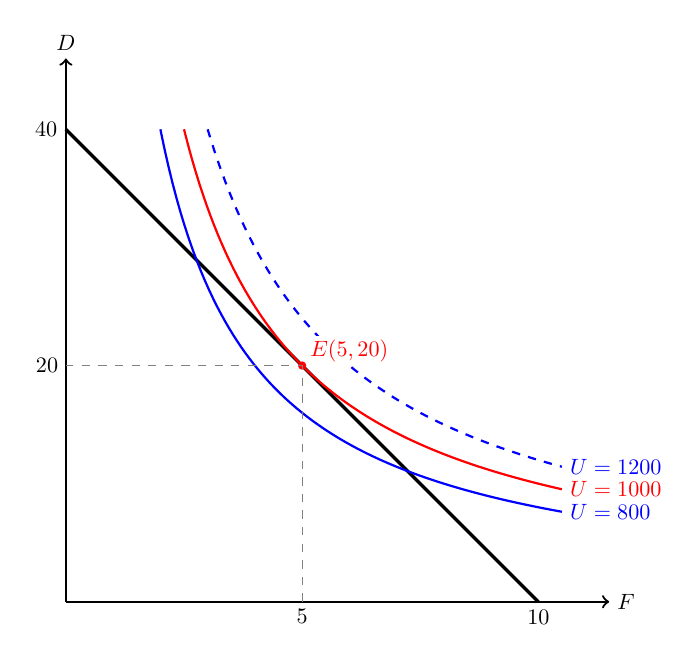
\begin{tikzpicture}[scale=0.6, every node/.style={scale=0.8}]
						\draw[->, thick] (0,0) -- (11.5,0) node[right] {$F$};
						\draw[->, thick] (0,0) -- (0,11.5) node[above] {$D$};
						
						% 缩放设定：纵轴 D 缩放为 1/4 (40->10)
						% 预算线 (y = 10 - x)
						\draw[very thick, black] (0,10) node[left] {$40$} -- (10,0) node[below] {$10$};
						
						% U=800 无差异曲线 (y' = 20/x)
						\draw[thick, blue, domain=2.0:10.5, samples=100] plot (\x, {20/\x}) node[right] {$U=800$};
						
						% U=1200 无差异曲线 (y' = 30/x)
						\draw[thick, blue, dashed, domain=3.0:10.5, samples=100] plot (\x, {30/\x}) node[right] {$U=1200$};
						
						% 最大效用 U=1000 无差异曲线，精确相切于 (5, 5) 对应实际的 (F=5, D=20)
						\draw[thick, red, domain=2.5:10.5, samples=100] plot (\x, {25/\x}) node[right] {$U=1000$};
						
						% 相切均衡点
						\fill[red] (5,5) circle (2.5pt);
						\node[above right, red, fill=white, inner sep=1.5pt,xshift=2pt] at (5,5) {$E(5, 20)$};
						
						% 辅助虚线
						\draw[dashed, gray] (5,0) node[below, black] {$5$} -- (5,5) -- (0,5) node[left, black] {$20$};
					\end{tikzpicture}
				\end{center}
				
				\textbf{a.} 根据效用函数，无差异曲线的数学表达式为：
				$$ U = 800 \implies 10DF = 800 \implies D = \frac{80}{F} $$
				$$ U = 1200 \implies 10DF = 1200 \implies D = \frac{120}{F} $$
				两者均为严格凸向原点的反比例双曲线，效用值为 1200 的曲线位于效用值为 800 的曲线的右上方。
				
				\textbf{b.} 预算约束方程为 $100D + 400F = 4000 \implies D = 40 - 4F$。
				
				\textbf{c.} 将预算线代入无差异曲线进行判断：
				由于最优效用发生在预算线与某条无差异曲线相切处，我们可以在 (d) 问中求得简能实现的最大效用为 $U = 1000$。
				因此，800 效用的无差异曲线与预算线有交点（例如 $D=20, F=4$），简有能力购买；而 1200 效用的曲线完全在预算线之外，简无法负担。
				
				\textbf{d.} 根据效用最大化的切点条件，边际替代率等于价格比：
				$$ MRS_{F,D} = \frac{MU_F}{MU_D} = \frac{D}{F} $$
				$$ \frac{D}{F} = \frac{P_F}{P_D} = 4 \implies D = 4F $$
				将其代入预算方程 $D + 4F = 40$，解得 $F = 5, D = 20$。最优组合为国内旅游 20 天，国外旅游 5 天。

				\item \textbf{朱利奥从消费食品（$F$）和衣服（$C$）中获得效用，由效用函数 $U(F,C)=FC$ 给出。另外，食品的价格为每单位2美元，衣服的价格为每单位10美元，朱利奥每星期的收入为50美元。\\
					a. 当朱利奥实现效用最大化时，食品对衣服的边际替代率是多少？请解释。\\
					b. 假设与效用最大化时的组合相比，朱利奥多购买了食品，少购买了衣服，他的食品对衣服的边际替代率会大于还是小于a部分的答案？请解释。}
				
				\textbf{答：}
				
				\textbf{a.}消费者实现效用最大化时，边际替代率等于市场价格比：
				$$ MRS_{F,C} = \frac{MU_F}{MU_C} = \frac{P_F}{P_C} = \frac{1}{5} $$
				在最优消费点处，由于价格约束，朱利奥主观上愿意放弃 $1$ 单位的衣服来换取额外 $5$ 单位的食品，这恰好等同于市场上购买 $1$ 单位食品所需要付出的衣服的真实机会成本。
				
				\textbf{b.}对于效用函数 $U(F,C) = FC$，其食品对衣服的边际替代率为：
				$$ MRS_{F,C} = \frac{MU_F}{MU_C} = \frac{C}{F} $$
				当朱利奥沿预算线向右下方移动（即 $F$ 增加、$C$ 减少）时，比值 $C/F$ 的分子减小、分母增大，因此 $MRS_{F,C}$ 会小于$0.2$。
				
				这反映了边际替代率递减规律。随着食品消费量的增加，食品的边际效用$MU_F$降低；同时衣服数量的减少使得衣服变得更为稀缺，其边际效用$MU_C$升高。因此，为获得额外一单位食品，他愿意放弃的衣服数量会越来越少（无差异曲线变得更加平缓）。

				\begin{center}
					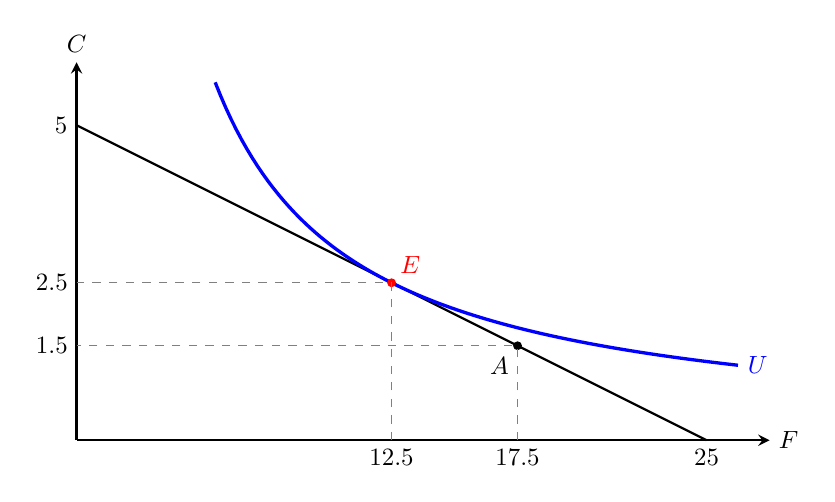
\begin{tikzpicture}[scale=0.8, >=stealth, every node/.style={scale=0.9}]

						\draw[->, thick] (0,0) -- (11,0) node[right] {$F$};
						\draw[->, thick] (0,0) -- (0,6) node[above] {$C$};

						\draw[thick, black] (0,5) node[left] {$5$} -- (10,0) node[below] {$25$};
						
						\draw[very thick, blue, domain=2.2:10.5, samples=100] plot (\x, {12.5/\x}) node[right] {$U$};
						
						\fill[red] (5,2.5) circle (2pt);
						\node[above right, red] at (5,2.5) {$E$};
						\draw[dashed, gray] (5,0) node[below, black] {$12.5$} -- (5,2.5) -- (0,2.5) node[left, black] {$2.5$};

						\fill[black] (7,1.5) circle (2pt);
						\node[above left,yshift=-15pt] at (7,1.5) {$A$};
						\draw[dashed, gray] (7,0) node[below, black] {$17.5$} -- (7,1.5) -- (0,1.5) node[left, black] {$1.5$};
					\end{tikzpicture}
				\end{center}
				
				\newpage
				\item \textbf{玛莉蒂斯从消费食品（$F$）和衣服（$C$）中得到的效用由 $U(F,C)=FC$ 给出。假设1990年她的收入为1200美元，食品和衣服的价格均为每单位1美元。但是到了2000年，食品价格上升至2美元，衣服价格上升至3美元。以100表示1990年的生活成本指数。请计算玛莉蒂斯在这样的偏好下，2000年的理想生活成本指数和拉氏指数。（提示：玛莉蒂斯将购买相同数量的食品和衣服。）}
				
				\textbf{答：}
				
				\textbf{1.计算基期（1990年）最优消费组合与效用水平}
				
				基期预算方程为 $F + C = 1200$。由效用最大化条件 $MRS_{F,C} = C/F = P_F/P_C = 1$，解得基期最优消费篮子为：
				$$ F_0 = 600, \quad C_0 = 600 $$
				玛莉蒂斯在基期获得的效用水平为：
				$$ U_0 = 600 \times 600 = 360000 $$
				
				\textbf{2.计算拉氏指数}
				
				拉氏指数采用基期的固定消费篮子 $(F_0, C_0)$ 作为权重，评估当期价格下购买该组合所需的成本涨幅：
				$$ \text{拉氏指数} = \frac{P_{F1}F_0 + P_{C1}C_0}{P_{F0}F_0 + P_{C0}C_0} \times 100 = \frac{2 \times 600 + 3 \times 600}{1200} \times 100 = 250 $$
				
				\textbf{3.计算理想生活成本指数}
				
				理想指数考量消费者为维持基期效用水平 $U_0 = 360000$ 不变时，在当期价格下所需的最小支出。
				在 2000 年的新价格下，最小化成本的切点条件为 $MRS_{F,C} = C/F = P_{F1}/P_{C1} = 2/3$，即 $C = 2F/3$。将其代入效用水平约束中：
				$$ F \times \left( \frac{2F}{3} \right) = 360000 \implies F_1 = 300\sqrt{6} \approx 734.85, \quad C_1 = 200\sqrt{6} \approx 489.90 $$
				维持该效用所需的当期最小总支出为：
				$$ E_1 = P_{F1}F_1 + P_{C1}C_1 = 2 \times 300\sqrt{6} + 3 \times 200\sqrt{6} \approx 2939.39 \text{ 美元} $$
				$$ \text{理想指数} = \frac{E_1}{E_0} \times 100 = \frac{2939.39}{1200} \times 100 \approx 245 $$
				
				拉氏指数为 250，理想生活成本指数约为 245。由于拉氏指数未能将消费者面对相对价格变化时进行的“消费替代行为”（用相对便宜的商品替代涨价商品）计算在内，它系统性地高估了真实的生活成本上升幅度。
		
		\end{enumerate}
	% =======================================================
	%                 第 4 章：个人需求与市场需求
	% =======================================================
	\chapter{个人需求与市场需求}
	
	\section{复习题}
	\begin{enumerate}[label=\textbf{\arabic*.}, leftmargin=*]
		\item \textbf{解释下面各项中每一项的区别：(1) 价格-消费曲线与需求曲线；(2) 个人需求曲线与市场需求曲线；(3) 收入-消费曲线与恩格尔曲线；(4) 收入效应与替代效应。}
		
		\textbf{答：}
		
		\textbf{(a) 价格-消费曲线 (PCC) 与需求曲线}
		
		价格-消费曲线是在消费者偏好、收入和其他商品价格不变的前提下，某一商品价格变动引起的效用最大化均衡点的轨迹，它反映了两种商品最优消费组合的变动路线。而需求曲线是由价格-消费曲线推导而来的，反映了单一商品需求量与其自身价格的一一对应关系，需求曲线上的每一点都满足效用最大化的均衡条件。
		\begin{center}
			\begin{tikzpicture}[scale=0.75, >=stealth, thick, every node/.style={scale=0.85}]
				% ==================== 左图：价格-消费曲线 (PCC) ====================
				\begin{scope}[xshift=0cm]
					% 横轴延长至9.5，防止标签重叠
					\draw[->] (0,0) -- (9.5,0) node[right] {$X$};
					\draw[->] (0,0) -- (0,5.5) node[above] {$Y$};
					
					% 预算线：假设 I=10, Py=2 (Y轴截距恒为5)
					% BL1: Px=2.5 (X截距=4)
					\draw[blue!60] (0,5) node[left, black] {$I/P_Y$} -- (4,0) node[below, black] {$P_{x1}$};
					% BL2: Px=1.66 (X截距=6)
					\draw[blue!60] (0,5) -- (6,0) node[below, black] {$P_{x2}$};
					% BL3: Px=1.11 (X截距=9)
					\draw[blue!60] (0,5) -- (9,0) node[below, black] {$P_{x3}$};
					
					% 均衡点：Y随X增加，使得PCC向右上方倾斜
					% E1: 在BL1上，选择 (2.0, 2.5)，斜率 m = 1.25
					\fill[black] (2.0, 2.5) circle (2pt) node[above right, fill=white, inner sep=1pt] {$E_1$};
					\draw[blue, domain=1.0:3.8, samples=100] plot (\x, {2.8125/(\x-0.5) + 0.625}) node[right] {$U_1$};
					
					% E2: 在BL2上，选择 (2.7, 2.75)，斜率 m = 5/6
					\fill[black] (2.7, 2.75) circle (2pt) node[above right, fill=white, inner sep=1pt] {$E_2$};
					\draw[blue, domain=1.6:5.0, samples=100] plot (\x, {(10/3)/(\x-0.7) + 13/12}) node[right] {$U_2$};
					
					% E3: 在BL3上，选择 (3.6, 3.0)，斜率 m = 5/9
					\fill[black] (3.6, 3.0) circle (2pt) node[above right, fill=white, inner sep=1pt] {$E_3$};
					\draw[blue, domain=2.2:7.5, samples=100] plot (\x, {4.05/(\x-0.9) + 1.5}) node[right] {$U_3$};
					
					% PCC 曲线：橙色，平滑连接且向右上方倾斜
					\draw[orange, dashed, ultra thick] plot[smooth] coordinates {(1.5, 2.1) (2.0, 2.5) (2.7, 2.75) (3.6, 3.0) (4.5, 3.25)} node[right, fill=white, inner sep=1pt] {PCC};
					
					% 辅助线
					\draw[dashed, gray] (2.0,0) -- (2.0, 2.5);
					\draw[dashed, gray] (2.7,0) -- (2.7, 2.75);
					\draw[dashed, gray] (3.6,0) -- (3.6, 3.0);
					
					\node[below] at (4.5,-1) {(a) 价格-消费曲线};
				\end{scope}
				
				% ==================== 右图：需求曲线推导 ====================
				\begin{scope}[xshift=11cm]
					\draw[->] (0,0) -- (9,0) node[right] {$Q_X$};
					\draw[->] (0,0) -- (0,5.5) node[above] {$P_X$};
					
					% 需求曲线：仅此线条为红色
					\draw[red, ultra thick] plot[smooth] coordinates {(1.2, 4.2) (2.0, 2.5) (2.7, 1.66) (3.6, 1.11) (6.0, 0.5)} node[right] {$D$};
					
					% 对应点：全黑
					\fill[black] (2.0, 2.5) circle (2pt) node[above right, fill=white, inner sep=1pt] {$E'_1$};
					\fill[black] (2.7, 1.66) circle (2pt) node[above right, fill=white, inner sep=1pt] {$E'_2$};
					\fill[black] (3.6, 1.11) circle (2pt) node[above right, fill=white, inner sep=1pt] {$E'_3$};
					
					% 辅助线与标注：黑色/灰色系
					\draw[dashed, gray] (2.0,0) node[below, black] {$X_1$} -- (2.0, 2.5) -- (0, 2.5) node[left, black] {$P_{x1}$};
					\draw[dashed, gray] (2.7,0) node[below, black] {$X_2$} -- (2.7, 1.66) -- (0, 1.66) node[left, black] {$P_{x2}$};
					\draw[dashed, gray] (3.6,0) node[below, black] {$X_3$} -- (3.6, 1.11) -- (0, 1.11) node[left, black] {$P_{x3}$};
					
					\node[below] at (4.5,-1) {(b) 需求曲线 };
				\end{scope}
			\end{tikzpicture}
		\end{center}
		
		\newpage
		\textbf{(b) 个人需求曲线与市场需求曲线}
		
		市场需求曲线是所有个体消费者需求曲线的水平加总。即在任意给定的价格水平下，市场总需求量等于该价格下所有个人的需求量之和。通常情况下，市场需求曲线比单条个人需求曲线更加平缓、更富有弹性。因为当价格下降时，不仅现有消费者会增加购买量，还会吸引新的消费者进入市场。
		\begin{center}
			\begin{tikzpicture}[scale=0.75, >=stealth, thick, every node/.style={scale=0.85}]
				\draw[->] (0,0) -- (12.5,0) node[right] {$Q$};
				\draw[->] (0,0) -- (0,5) node[above] {$P$};
				
				% 个人需求曲线 D_A: P = 4 - Q_A
				\draw[blue] (0,4) -- (4,0) node[below left, yshift=15pt,xshift=-5pt] {$D_A$};
				% 个人需求曲线 D_B: P = 4 - 0.5 Q_B
				\draw[red] (0,4) -- (8,0) node[below left,yshift=25pt] {$D_B$};
				% 市场需求曲线 D_M: Q_M = 12 - 3P => P = 4 - Q/3
				\draw[green!60!black, very thick] (0,4) -- (12,0) node[below left,yshift=25pt] {$D_{\text{市场}}$};
				
				% 水平加总示例 P=2
				\draw[dashed, gray] (0,2) node[left, black] {$P_0$} -- (6,2);
				\fill[black] (2,2) circle (1.5pt) node[above right] {$Q_A$};
				\fill[black] (4,2) circle (1.5pt) node[above right] {$Q_B$};
				\fill[black] (6,2) circle (1.5pt) node[above right] {$Q_A+Q_B$};
				
				\draw[dashed, gray] (2,2) -- (2,0) node[below, black] {$2$};
				\draw[dashed, gray] (4,2) -- (4,0) node[below, black] {$4$};
				\draw[dashed, gray] (6,2) -- (6,0) node[below, black] {$6$};
			\end{tikzpicture}
		\end{center}
		
		\textbf{(c) 收入-消费曲线 (ICC) 与恩格尔曲线}
		
		收入-消费曲线描绘的是商品相对价格不变时，随着人们收入水平的改变而产生最优选择的各种商品组合。恩格尔曲线则表示将其中的收入与单一商品的需求量单独提取出来画成的映射关系。两者区别主要在于：需求曲线考虑了价格对需求量的影响；恩格尔曲线考虑了收入对需求量的影响，正常品的恩格尔曲线向上倾斜，劣等品的恩格尔曲线向下倾斜。
		\begin{center}
			\begin{tikzpicture}[scale=0.8, >=stealth, thick, every node/.style={scale=0.85}]
				% ==================== 左图：收入-消费曲线 (ICC) ====================
				\begin{scope}[xshift=0cm]
					\draw[->] (0,0) -- (7,0) node[right] {$X$};
					\draw[->] (0,0) -- (0,7) node[above] {$Y$};
					
					% 预算线 (平行外移，截距缩小为 3, 4.5, 6，防溢出)
					\draw[red] (0,3) -- (3,0);
					\draw[red] (0,4.5) -- (4.5,0);
					\draw[red] (0,6) -- (6,0);
					
					% 无差异曲线 (精确相切计算，反比例系数分别为 2.25, 5.0625, 9)
					\draw[blue, domain=0.7:3.2, samples=100] plot (\x, {2.25/\x}) node[right] {$U_1$};
					\draw[blue, domain=1.2:4.7, samples=100] plot (\x, {5.0625/\x}) node[right] {$U_2$};
					\draw[blue, domain=1.6:6.0, samples=100] plot (\x, {9/\x}) node[right] {$U_3$};
					
					% ICC 曲线
					\draw[orange, dashed, very thick] (0,0) -- (4.5,4.5) node[above right, fill=white, inner sep=1pt] {ICC};
					
					% 均衡点 (1.5, 1.5), (2.25, 2.25), (3, 3)
					\fill (1.5,1.5) circle (2pt) node[above left, fill=white, inner sep=1pt] {$E_1$};
					\fill (2.25,2.25) circle (2pt) node[above left, fill=white, inner sep=1pt] {$E_2$};
					\fill (3,3) circle (2pt) node[above left, fill=white, inner sep=1pt] {$E_3$};
					
					% 投影辅助线 (明确标出 X_1, X_2, X_3)
					\draw[dashed, gray] (1.5,0) node[below, black] {$X_1$} -- (1.5,1.5);
					\draw[dashed, gray] (2.25,0) node[below, black] {$X_2$} -- (2.25,2.25);
					\draw[dashed, gray] (3,0) node[below, black] {$X_3$} -- (3,3);
					
					\node[below] at (3.5,-0.8) {(a) 收入-消费曲线};
				\end{scope}
				
				% ==================== 右图：恩格尔曲线 ====================
				\begin{scope}[xshift=8.5cm]
					\draw[->] (0,0) -- (6,0) node[right] {$X$};
					\draw[->] (0,0) -- (0,6) node[above] {$I$ (收入)};
					
					% 恩格尔曲线 (等比例映射在画布内)
					\draw[purple, very thick] (0,0) -- (4.5, 4.5) node[right, fill=white, inner sep=1pt] {恩格尔曲线};
					
					% 收入对应点
					\fill (1.5,1.5) circle (2pt) node[above left] {$A$};
					\fill (2.25,2.25) circle (2pt) node[above left] {$B$};
					\fill (3,3) circle (2pt) node[above left] {$C$};
					
					% 投影辅助线 (保持横坐标绝对一致)
					\draw[dashed, gray] (1.5,0) node[below, black] {$X_1$} -- (1.5,1.5) -- (0,1.5) node[left, black] {$I_1$};
					\draw[dashed, gray] (2.25,0) node[below, black] {$X_2$} -- (2.25,2.25) -- (0,2.25) node[left, black] {$I_2$};
					\draw[dashed, gray] (3,0) node[below, black] {$X_3$} -- (3,3) -- (0,3) node[left, black] {$I_3$};
					
					\node[below] at (3,-0.8) {(b) 恩格尔曲线 (正常品)};
				\end{scope}
			\end{tikzpicture}
		\end{center}
		
		\textbf{(d) 收入效应与替代效应}
		
		\textbf{答：}
		商品价格变动引发的总效应可分解为替代效应与收入效应。替代效应是纯粹由相对价格变动引起的需求量变化，表现为同一条无差异曲线上的点移动。收入效应是由实际购买力改变引起的需求量变化，表现为不同无差异曲线之间的跃迁。根据两者的方向与大小关系，商品可分为正常品（两者同向增加）、一般劣等品（收入效应反向但较弱）与吉芬品（收入效应反向且起主导作用）。
		
		\begin{center}
			\begin{tikzpicture}[scale=0.6, >=stealth, thick, every node/.style={scale=0.75}]
				% ==================== 图1：正常品 ====================
				\begin{scope}[xshift=0cm]
					\draw[->] (0,0) -- (8.5,0) node[right] {$X$};
					\draw[->] (0,0) -- (0,5.5) node[above] {$Y$};
					
					% 预算线
					\draw[red] (0,4) -- (4,0);
					\draw[red] (0,4) -- (8,0);
					\draw[red, dashed] (0,2.83) -- (5.66,0); 
					
					% 无差异曲线
					\draw[blue, domain=1.1:4.5, samples=100] plot (\x, {4/\x}) node[right] {$U_1$};
					\draw[blue, domain=2.2:7.5, samples=100] plot (\x, {8/\x}) node[right] {$U_2$};
					
					% 均衡点
					\fill (2,2) circle (2pt) node[above right] {$E_1$};
					\fill (2.83,1.41) circle (2pt) node[below left, xshift=-1pt] {$E_2$};
					\fill (4,2) circle (2pt) node[above right] {$E_3$};
					
					% 投影与标注
					\draw[dashed, gray] (2,2) -- (2,-0.2) node[below, black] {$x_1$};
					\draw[dashed, gray] (2.83,1.41) -- (2.83,-0.2) node[below, black] {$x_2$};
					\draw[dashed, gray] (4,2) -- (4,-0.2) node[below, black] {$x_3$};
					
					% 效应箭头
					\draw[->, orange] (2,-0.6) -- (2.83,-0.6) node[midway, below] {替代};
					\draw[->, purple] (2.83,-0.6) -- (4,-0.6) node[midway, below] {收入};
					\node[below] at (4,-1.8) {(a) 正常品};
				\end{scope}
				
				% ==================== 图2：劣等品 (非吉芬) ====================
				\begin{scope}[xshift=9cm]
					\draw[->] (0,0) -- (8.5,0) node[right] {$X$};
					\draw[->] (0,0) -- (0,5.5) node[above] {$Y$};
					
					% 预算线
					\draw[red] (0,4) -- (4,0);
					\draw[red] (0,4) -- (8,0);
					\draw[red, dashed] (0,2.83) -- (5.66,0);
					
					% 无差异曲线
					\draw[blue, domain=1.1:4.5, samples=100] plot (\x, {4/\x}) node[right] {$U_1$};
					\draw[blue, domain=1.55:7.0, samples=100] plot (\x, {0.5/(\x-1.4) + 2.3}) node[right] {$U_2$};
					
					% 均衡点 (E3在E1和E2之间)
					\fill (2,2) circle (2pt) node[above right,xshift=-6pt] {$E_1$};
					\fill (2.83,1.41) circle (2pt) node[above right, fill=white, inner sep=1pt] {$E_2$};
					\fill (2.4,2.8) circle (2pt) node[above right] {$E_3$};
					
					% 投影与标注
					\draw[dashed, gray] (2,2) -- (2,-0.2) node[below, black] {$x_1$};
					\draw[dashed, gray] (2.83,1.41) -- (2.83,-0.2) node[below, black] {$x_2$};
					\draw[dashed, gray] (2.4,2.8) -- (2.4,-0.2) node[below, black] {$x_3$};
					
					% 效应箭头 (分层防止重叠)
					\draw[->, orange] (2,-0.6) -- (2.83,-0.6) node[midway, below] {替代};
					\draw[->, purple] (2.83,-1.2) -- (2.4,-1.2) node[midway, below] {收入};
					\node[below] at (4,-1.8) {(b) 一般劣等品};
				\end{scope}
				
				% ==================== 图3：吉芬品 ====================
				\begin{scope}[xshift=18cm]
					\draw[->] (0,0) -- (8.5,0) node[right] {$X$};
					\draw[->] (0,0) -- (0,5.5) node[above] {$Y$};
					
					% 预算线
					\draw[red] (0,4) -- (4,0);
					\draw[red] (0,4) -- (8,0);
					\draw[red, dashed] (0,2.83) -- (5.66,0);
					
					% 无差异曲线
					\draw[blue, domain=1.1:4.5, samples=100] plot (\x, {4/\x}) node[right] {$U_1$};
					\draw[blue, domain=0.85:5.5, samples=100] plot (\x, {0.32/(\x-0.7) + 2.85}) node[right] {$U_2$};
					
					% 均衡点 (E3在E1左侧)
					\fill (2,2) circle (2pt) node[above right] {$E_1$};
					\fill (2.83,1.41) circle (2pt) node[above right] {$E_2$};
					\fill (1.5,3.25) circle (2pt) node[above right] {$E_3$};
					
					% 投影与标注
					\draw[dashed, gray] (2,2) -- (2,-0.2) node[below, black] {$x_1$};
					\draw[dashed, gray] (2.83,1.41) -- (2.83,-0.2) node[below, black] {$x_2$};
					\draw[dashed, gray] (1.5,3.25) -- (1.5,-0.2) node[below, black] {$x_3$};
					
					% 效应箭头 (分层防止重叠)
					\draw[->, orange] (2,-0.6) -- (2.83,-0.6) node[midway, below] {替代};
					\draw[->, purple] (2.83,-1.2) -- (1.5,-1.2) node[midway, below] {收入};
					\node[below] at (4,-1.8) {(c) 吉芬品};
				\end{scope}
			\end{tikzpicture}
		\end{center}
		
		\item \textbf{假定某人在食品和衣服这两种商品上花费他全部的预算。两种商品是否可能都为劣等品？请说明原因。}
		
		\textbf{答：}
		不可能。假设消费者仅消费食品与衣服即 $X$ 和 $Y$，其面临的预算约束方程为：
		$$ P_X X + P_Y Y = I $$
		其中，$P_X$ 和 $P_Y$ 分别为食品 $X$ 和衣服 $Y$ 的价格，$I$ 为消费者的总收入。
		
		将预算约束等式两边对收入 $I$ 求偏导得：
		$$ P_X \frac{\partial X}{\partial I} + P_Y \frac{\partial Y}{\partial I} = 1 $$
		
		若一种商品为劣等品，则其需求量随收入的增加而减少，即需求对收入的偏导数小于零。假设 $X$ 和 $Y$ 均为劣等品，则必然有：
		$$ \frac{\partial X}{\partial I} < 0 \quad \text{且} \quad \frac{\partial Y}{\partial I} < 0 $$
		
		由于商品的价格在现实市场中严格为正（$P_X > 0, P_Y > 0$），上述不等式意味着：
		$$ P_X \frac{\partial X}{\partial I} < 0 \quad \text{且} \quad P_Y \frac{\partial Y}{\partial I} < 0 $$
		
		将两式相加，必然推导出：
		$$ P_X \frac{\partial X}{\partial I} + P_Y \frac{\partial Y}{\partial I} < 0 $$
		
		这一不等式与我们之前求导得出的恒等式产生了逻辑矛盾。因此原假设不成立，在消费者只消费两种商品的情况下，这两种商品不可能同时为劣等品，其中至少有一种必须是正常品，以吸收增加的收入份额。
		
		\item \textbf{解释下述说法是对还是错：(1) 当人们沿着其需求曲线往下移动时，边际替代率递减。(2) 当人们沿着其需求曲线往下移动时，效用水平上升。(3) 恩格尔曲线总是向上倾斜的。}
		
		\textbf{答：}
		\begin{enumerate}[label=(\arabic*), leftmargin=*]
			\item 正确。当消费者实现效用最大化时，其边际替代率等于相对价格之比，即 $MRS_{XY} = P_X/P_Y$。当消费者沿着商品 $X$ 的需求曲线向下移动时，意味着商品 $X$ 的自身价格 $P_X$ 正在不断下降。在其他商品价格 $P_Y$ 保持不变的情况下，相对价格比 $P_X/P_Y$ 减小，因此消费者对该商品的边际替代率必然是递减的。
			\item 正确。当人们沿着某商品的需求曲线向下移动时，表明该商品的价格正在下降。在名义收入和其他条件不变的情况下，价格下降使得消费者的实际购买力增强，预算线向外旋转。这种预算集的扩张允许消费者触及更高水平的无差异曲线，从而获得更高的总效用。
			\item 错误。恩格尔曲线的形状完全取决于商品的收入弹性性质。对于正常品，需求量随收入的增加而增加，恩格尔曲线表现为向上倾斜；但对于劣等品，需求量随收入的增加反而下降，其恩格尔曲线会向左上方弯曲，呈现出向下倾斜的形态。
		\end{enumerate}
		
		\item \textbf{一场摇滚音乐会的门票售价为 10 美元。但在该价格下，需求远大于可供的门票数量，那么额外一张门票的价值或边际收益是大于、小于还是等于 10 美元？你怎样来确定这一价值呢？}
		
		\textbf{答：}
		额外一张门票的经济价值大于 10 美元。
		
		商品的边际价值是由消费者为了得到该商品愿意支付最高的价格来决定的，假如一张门票在官方限价上涨10美元且导致了市场严重供不应求时，那么能让市场真正出清的均衡价格远远大于10美元。这个时候许多未买到票的人在私下交易或心理预估中也已经愿意支付超过官方定价的金额。因此，有这样一张门票的真实价值必然大于10美元，可以通过观察黑市的交易价格或问卷调查消费者支付意愿的最高价格来确定。
		
		\item \textbf{在下面的商品组合中，哪些是互补品？哪些是替代品？在不同的情形下，它们可以两者兼而有之吗？讨论一下。a. 一堂数学课和一堂经济学课；b. 网球和网球拍；c. 牛排和龙虾；d. 目的地相同的飞机和火车；e. 培根和鸡蛋。}
		
		\textbf{答：}
		微观经济学中，替代品与互补品的核心判断标准是需求交叉价格弹性。若一种商品价格上升会导致另一种商品需求量增加（交叉价格弹性 $E_{XY} > 0$），二者为替代品，可相互替代满足同类需求；若一种商品价格上升会导致另一种商品需求量减少（交叉价格弹性 $E_{XY} < 0$），二者为互补品，需搭配使用才能发挥完整效用。商品关系并非绝对，会随消费情境变化相互转化。具体分析如下：
		\begin{enumerate}[label=\alph*., leftmargin=*]
			\item 一堂数学课和一堂经济学课：通常用作替代品，如果同一时间上数学课，那么不可能同时上经济学课。但是在长期的学习规划中，两者都属于互补品：如果经济学以数学知识为先修基础，随着学生选择经济学课难度或成本增加，数学课需求量也会减少。
			\item 网球和网球拍：典型的完全互补品，只有按固定比例配合使用才能满足网球运动的需求，缺少任何一方都不可以单独产生效用，交叉价格弹性很小，几乎无法转化为替代品。
			\item 牛排和龙虾：通常是替代品。二者作为正餐的主菜都满足消费者对高蛋白肉类的需求，大多数情况下消费者选择二选一，牛排涨价会带动龙虾增加；但某些消费场景（如西餐厅开办“海陆双拼”套餐），二者被打包为一个消费组合，此时牛排涨价会带动整个套餐的需求量减少，带动龙虾减少，二者则成为了互补品。
			\item 目的地相同的飞机和火车：通常是替代品。二者均提供点对点的空间位移服务，在直达出行中满足同一需求，机票降价会导致火车票的需求量下降。但在长途联程旅行中二者则可以转换成为互补品，如乘坐飞机先到达中转城市再到达火车所在城市，此时机票涨价会带动整个行程的需求量减少，带动中转火车票的需求量减少。
			\item 培根和鸡蛋：通常是互补品。二者经常搭配食用，鸡蛋涨价会导致培根的需求量同步下降，但当消费者只需要补充蛋白质为单一需求时，二者也能够变换成为替代品，如果鸡蛋价格大幅上涨，那么人们就会选择多吃培根来代替鸡蛋来补充蛋白质。
		\end{enumerate}
		
		\newpage
		\item \textbf{消费者每月花费固定数额在下列成对商品上。对于每一对商品，说明它们是替代品还是互补品。a. 咖啡和糖；b. 咖啡和茶；c. 汉堡和薯条；d. 可口可乐和百事可乐。}
		
		\textbf{答：}
		\begin{enumerate}[label=\alph*., leftmargin=*]
			\item 互补品：咖啡与糖通常搭配饮用，咖啡价格上涨会导致糖的需求量下降。
			\item 替代品：二者均满足提神解渴的需求，咖啡价格上涨会导致茶的需求量上升。
			\item 互补品：汉堡与薯条是快餐的经典搭配，汉堡价格上涨会导致薯条的需求量下降。
			\item 完全替代品：二者功能与口感高度同质化，可口可乐价格略微上涨就会导致百事可乐需求量大幅上升。
		\end{enumerate}
		
		\item \textbf{指出下列事件会引起美国国产服装需求曲线的移动，还是需求量的变动（沿需求曲线移动）。a. 取消对外国服装进口的配额；b. 美国消费者收入增加；c. 全行业生产国内服装的成本降低，导致服装价格下降。}
		
		\textbf{答：}
		\begin{enumerate}[label=\alph*., leftmargin=*]
			\item 需求曲线向左移动（需求的变动）：取消进口配额后，外国服装供给增加、价格下降。由于替代品变得更加便宜，消费者会转向购买外国服装，导致在任意给定价格下，对美国国产服装的需求均减少，需求曲线向左平移。
			\item 需求曲线向右移动（需求的变动）：服装通常属于正常商品。美国消费者收入增加会提升其整体购买力，使得任意价格水平下对国产服装的需求量均上升，需求曲线向右平移。
			\item 沿需求曲线向下移动（需求量的变动）：生产成本降低导致国产服装自身价格下降。由商品自身价格变动引起的购买数量增加，表现为沿着原有的需求曲线向右下方滑动，不会引起需求曲线本身的位移。
		\end{enumerate}
		
		\item \textbf{对于下列商品，哪一种商品的价格上涨会导致较大的收入效应？哪一种会导致较大的替代效应？解释原因。a. 盐；b. 住房；c. 剧院门票；d. 食物。}
		
		\textbf{答：}
		\begin{center}
			\renewcommand{\tabularxcolumn}[1]{m{#1}}
			\begin{tabularx}{\textwidth}{c c c >{\arraybackslash}X}
				\toprule
				\textbf{商品} & \textbf{收入效应} & \textbf{替代效应} & \textbf{核心原因} \\
				\midrule
				盐 & 极小 & 极小 & 占消费者预算比例极低（收入效应小），且作为调味必需品几乎无替代品（替代效应小）。 \\
				住房 & 最大 & 较小 & 占家庭总预算比例最高，价格上涨会大幅压缩实际购买力（收入效应大）；但在短期内极难找到合适的居住替代品（替代效应小）。 \\
				剧院门票 & 中等 & 最大 & 占预算比例适中；但作为休闲娱乐消费，存在大量高度同质化的替代品（如看电影、听演唱会等，替代效应大）。 \\
				食物 & 较大 & 较小 & 占家庭整体预算比例较高（收入效应大）；尽管不同食物间可以相互替代，但作为整体的“食物”是生存刚需，没有其他类别的替代品（整体替代效应小）。 \\
				\bottomrule
			\end{tabularx}
		\end{center}
		
		\newpage
		\item \textbf{假设政府对汽油征收 20\% 的从价税，同时将征收的税款以每人 160 美元的一次性退税方式返还给消费者。如果消费者的偏好是凸的，那么消费者的境况是得到改善还是恶化？用预算线和无差异曲线作图说明。}
		
		\textbf{答：}
		消费者的境况将恶化。这是显示偏好理论与税收效率损失的经典应用，具体分析如下：
		
		\begin{enumerate}[label=\arabic*., leftmargin=*]
			\item 预算线变动：征税增加了汽油的相对价格，导致预算线绕纵轴截距点向内旋转。随后的退税作为收入补偿，使预算线向外平行移动。
			\item 均衡位置：在政府实行收入中性政策（即退税额等于消费者在新均衡下的实际缴税额）时，最终的预算线 $L_1$ 必然经过新均衡点 $E_1$，且该点刚好位于原预算线 $L_0$ 上。
			\item 结论：由于 $E_0$ 是原预算线 $L_0$ 上唯一的效用最大化点，任何位于 $L_0$ 上且受相对价格扭曲影响的新选择 $E_1$，其对应的效用水平 $U_1$ 必然低于初始效用 $U_0$。因此，消费者的境况变坏了。
		\end{enumerate}
		
		\begin{center}
			\begin{tikzpicture}[scale=0.85, >=stealth, thick, every node/.style={scale=0.85}]
				% 1. 坐标轴与基本框架
				\draw[->] (0,0) -- (11,0) node[right] {汽油 ($X$)};
				\draw[->] (0,0) -- (0,9) node[above] {其他商品 ($Y$)};
				
				% 2. 初始预算线 L0: y = 6 - 0.5x (黑色实线，斜率平缓)
				\coordinate (A) at (0,6);
				\coordinate (B) at (10,1); 
				\draw[black, very thick] (A) node[left] {$M/P_y$} -- (B) node[right] {$L_0$};
				
				% 3. 价格旋转示意 (灰色虚线): 汽油价格上涨，预算线变陡 y = 6 - x
				\coordinate (C) at (6,0);
				\draw[dashed, gray!80, thick] (A) -- (C);
				
				% 4. 最终预算线 L1 (蓝色实线): 退税后平移，斜率与虚线相同 y = 8 - x
				\coordinate (D) at (0,8);
				\coordinate (E) at (8,0);
				\draw[blue, very thick] (D) -- (E) node[below] {$L_1$};
				
				% 5. 均衡点与无差异曲线
				% 原均衡 E0 (6,3)
				\coordinate (E0) at (6,3);
				\fill (E0) circle (2pt);
				\node[above right, fill=white, inner sep=1pt, xshift=2pt] at (E0) {$E_0$};
				\draw[blue!50, very thick, domain=3.2:10.5, samples=100] plot (\x, {18/\x}) node[right] {$U_0$};
				
				% 新均衡 E1 (4,4)
				% E1 恰好落在 L0 上 (4*0.5+4=6) 且为 L1 的切点
				\coordinate (E1) at (4,4);
				\fill (E1) circle (2pt);
				\node[below left, fill=white, inner sep=1pt, xshift=-2pt, yshift=-2pt] at (E1) {$E_1$};
				\draw[red!50, very thick, domain=2.2:9.5, samples=100] plot (\x, {16/\x}) node[right,yshift=-3pt] {$U_1$};
				
				% 6. 辅助标注与投影线
				% 投影虚线
				\draw[dotted, gray, thick] (E1) -- (4,0) node[below, black] {$x_1$};
				\draw[dotted, gray, thick] (E1) -- (0,4) node[left, black] {$y_1$};
				
				% 箭头指示
				\draw[->, gray, thick] (7, 2.5) to[bend left=15] (4, 2) node[below right, fill=white, inner sep=1pt,yshift=-3pt,xshift=-3pt] {价格上涨旋转};
				\draw[->, gray, thick] (1, 5) -- (2, 6) node[midway, left=4pt,xshift=7pt,yshift=20pt] {退税平移};
				
			\end{tikzpicture}
		\end{center}
		
		\item \textbf{解释为什么下列各组人对商业经济学家协会的成员资格需求具有不同的价格弹性：a. 学生；b. 初级经理；c. 高级经理。}
		
		\textbf{答：}
		需求价格弹性的大小主要由其预算和需求决定，排序为：\text{学生} > \text{初级经理} > \text{高级经理}。
		\begin{enumerate}[label=\alph*., leftmargin=*]
			\item 学生：弹性最大。会员费占学生有限收入的比重很高，且学生可以通过图书馆或互联网获取替代性资源，价格上涨会显著减少其加入意愿。
			\item 初级经理：弹性中等。其收入水平高于学生，且职业发展初期需要建立人脉和获取行业资讯，需求刚性有所增加。
			\item 高级经理：弹性最小。会员费相对于其高额收入几乎可以忽略不计；更重要的是，协会成员资格往往是身份象征或高层社交的门槛，具有极强的不可替代性。
		\end{enumerate}
		
		\newpage
		\item \textbf{解释下列各组商品中，哪一种商品的需求更富有价格弹性，并说明原因。a. 某一特定品牌的牙膏和普通牙膏；b. 汽油在短期内的需求和在长期内的需求。}
		
		\textbf{答：}
		\begin{enumerate}[label=\alph*., leftmargin=*]
			\item 某一特定品牌的牙膏更富有弹性。因为特定品牌（如高露洁）有众多的近似替代品（如佳洁士、黑人），价格微涨即会导致消费者转向竞品。而普通牙膏作为大类，缺乏替代品，需求相对缺乏弹性。
			\item 长期内的汽油需求更富有弹性。短期内，消费者的出行习惯和车辆类型相对固定；长期内，消费者可以更换省油车型、改用电动车或改变居住地点以利用公共交通，从而对价格变化做出更充分的反应。
		\end{enumerate}
		
		\item \textbf{什么是正网络外部性和负网络外部性？各举一个例子说明。}
		
		\textbf{答：}
		网络外部性是指一个消费者的需求受其他消费者购买行为影响的现象。
		\begin{enumerate}[label=\arabic*., leftmargin=*]
			\item \textbf{正网络外部性}：指一名消费者对商品的需求随其他消费者购买数量的增加而增加。比如社交软件（如微信）。用户越多，每个用户的沟通价值越高（协同效应），从而吸引更多人使用。

			\item \textbf{负网络外部性}：指一名消费者对商品的需求随其他消费者购买数量的增加而减少。比如拥挤效应。例如公共景点的游览或热门餐厅的排队，随着人数增加，等待时间和环境恶化降低了每个人的效用。

		\end{enumerate}
		
		
		
	\end{enumerate}
	
	\section{练习题}
	\begin{enumerate}[label=\textbf{\arabic*.}, leftmargin=*]
		\item \textbf{某人每月预算150美元用于购买红酒和书籍，书籍价格固定为10美元/本。不同红酒价格下的最优消费组合如下表所示。请推导并画出红酒的价格-消费曲线（PCC）与需求曲线。}
		\begin{center}
			\begin{tabularx}{0.9\textwidth}{>{\centering\arraybackslash}X >{\centering\arraybackslash}X >{\centering\arraybackslash}X >{\centering\arraybackslash}X >{\centering\arraybackslash}X}
				\toprule
				\textbf{红酒价格} & \textbf{书籍价格} & \textbf{红酒数量} & \textbf{书籍数量} & \textbf{预算} \\
				\midrule
				10 & 10 & 7 & 8 & 150 \\
				12 & 10 & 5 & 9 & 150 \\
				15 & 10 & 4 & 9 & 150 \\
				20 & 10 & 2 & 11 & 150 \\
				\bottomrule
			\end{tabularx}
		\end{center}
		
		\textbf{答：}
		设红酒数量为 $Q_R$，书籍数量为 $Q_B$，预算约束为 $P_R Q_R + 10Q_B = 150$。随着 $P_R$ 从 10、12、15 升至 20，预算线的纵轴截距固定在 15，横轴截距分别变为 15、12.5、10 和 7.5。
		
		将四个效用最大化切点 $(7,8)$、$(5,9)$、$(4,9)$、$(2,11)$ 依次连接，即可得到红酒的价格-消费曲线。
		
		从上述均衡状态中提取红酒的 $(P_R, Q_R)$ 价格与需求量组合数据，在坐标平面上描点连线，即可得到红酒的需求曲线。
		
		\begin{center}
			\begin{tikzpicture}[>=stealth, thick, every node/.style={scale=0.8}]
				% === 左图：价格-消费曲线 (压缩比例) ===
				\begin{scope}[x=0.25cm, y=0.25cm] % 设置单位长度为0.25cm，显著缩小物理尺寸
					\draw[->] (0,0) -- (17,0) node[right] {$Q_R$};
					\draw[->] (0,0) -- (0,17) node[above] {$Q_B$};
					
					% 预算线
					\draw[gray!60] (0,15) node[left, black] {$15$} -- (15,0) node[below, black] {$15$};
					\draw[gray!60] (0,15) -- (12.5,0) node[below, black] {$12.5$};
					\draw[gray!60] (0,15) -- (10,0) node[below, black] {$10$};
					\draw[gray!60] (0,15) -- (7.5,0) node[below, black] {$7.5$};
					
					% 精确相切的无差异曲线 (模型: y = c + k/x)
					\draw[blue, dashed, domain=3.3:14.5, samples=50] plot (\x, {1 + 49/\x});
					\draw[blue, dashed, domain=2.2:11.5, samples=50] plot (\x, {3 + 30/\x});
					\draw[blue, dashed, domain=1.7:9.5, samples=50] plot (\x, {3 + 24/\x});
					\draw[blue, dashed, domain=0.9:6.5, samples=50] plot (\x, {7 + 8/\x});
					
					% 均衡点
					\fill (7,8) circle (2pt);
					\fill (5,9) circle (2pt);
					\fill (4,9) circle (2pt);
					\fill (2,11) circle (2pt);
					
					% PCC曲线
					\draw[red, very thick] (7,8) -- (5,9) -- (4,9) -- (2,11);
					\node[above right, red, fill=white, inner sep=0.5pt] at (5.5,8.8) {PCC};
					
					\node[below] at (8,-2) {(a) 价格-消费曲线};
				\end{scope}
				
				% === 右图：需求曲线 (加大间隔防止重叠) ===
				% 间隔计算：左图宽度约 17*0.25=4.25cm，将xshift设为 6.5cm 左右可保证安全距离
				\begin{scope}[x=0.25cm, y=0.25cm, xshift=6.5cm] 
					\draw[->] (0,0) -- (10,0) node[right] {$Q_R$};
					\draw[->] (0,0) -- (0,12) node[above] {$P_R$};
					
					% 虚线投影 (价格按 1:0.5 比例缩放展示)
					\draw[dashed, gray!80, thin] (7,0) node[below, black] {$7$} -- (7,5) -- (0,5) node[left, black] {$10$};
					\draw[dashed, gray!80, thin] (5,0) node[below, black] {$5$} -- (5,6) -- (0,6) node[left, black] {$12$};
					\draw[dashed, gray!80, thin] (4,0) node[below, black] {$4$} -- (4,7.5) -- (0,7.5) node[left, black] {$15$};
					\draw[dashed, gray!80, thin] (2,0) node[below, black] {$2$} -- (2,10) -- (0,10) node[left, black] {$20$};
					
					% 需求点
					\fill (7,5) circle (2pt);
					\fill (5,6) circle (2pt);
					\fill (4,7.5) circle (2pt);
					\fill (2,10) circle (2pt);
					
					% 需求曲线
					\draw[purple, very thick] (7,5) -- (5,6) -- (4,7.5) -- (2,10);
					\node[above right, purple] at (4,7.5) {$D$};
					
					\node[below] at (5,-2) {(b) 需求曲线};
				\end{scope}
			\end{tikzpicture}
		\end{center}
		
		\item \textbf{某人消费衣服和食品，衣服价格固定为10美元/件，食品价格固定为2美元/单位。不同收入下的最优消费组合如下表所示。请推导并画出衣服的收入-消费曲线（ICC）与恩格尔曲线。}
		\begin{center}
			\begin{tabularx}{0.9\textwidth}{>{\centering\arraybackslash}X >{\centering\arraybackslash}X >{\centering\arraybackslash}X >{\centering\arraybackslash}X >{\centering\arraybackslash}X}
				\toprule
				\textbf{衣服价格} & \textbf{食品价格} & \textbf{衣服数量} & \textbf{食品数量} & \textbf{收入} \\
				\midrule
				10 & 2 & 6 & 20 & 100 \\
				10 & 2 & 8 & 35 & 150 \\
				10 & 2 & 11 & 45 & 200 \\
				10 & 2 & 15 & 50 & 250 \\
				\bottomrule
			\end{tabularx}
		\end{center}
		
		\textbf{答：}
		设衣服为 $Q_C$，食品为 $Q_F$，预算约束为 $10Q_C + 2Q_F = I$。当收入从 100 增至 250 时，预算线保持斜率 $-5$ 平行向外移动。
		
		将四个收入水平下的均衡切点 $(6,20)$、$(8,35)$、$(11,45)$、$(15,50)$ 连接，得到衣服的收入-消费曲线。两种商品数量均随收入增加而增加，说明两者均为正常品。
		
		提取 $(I, Q_C)$ 的组合数据，绘制在横轴为需求量、纵轴为收入的坐标系中，即得到衣服的恩格尔曲线。
		
		\begin{center}
			\begin{tikzpicture}[>=stealth, thick, every node/.style={scale=0.8}]
				% === 左图：收入-消费曲线 (严格限制物理尺寸) ===
				% 设定 x=0.18cm (横轴28最大约5cm)，y=0.035cm (纵轴145最大约5cm)
				\begin{scope}[x=0.18cm, y=0.035cm] 
					\draw[->] (0,0) -- (28,0) node[right] {$Q_C$};
					\draw[->] (0,0) -- (0,145) node[above] {$Q_F$};
					
					% 预算线
					\draw[gray!60] (0,50) node[left, black] {$50$} -- (10,0) node[below, black] {$10$};
					\draw[gray!60] (0,75) node[left, black] {$75$} -- (15,0) node[below, black] {$15$};
					\draw[gray!60] (0,100) node[left, black] {$100$} -- (20,0) node[below, black] {$20$};
					\draw[gray!60] (0,125) node[left, black] {$125$} -- (25,0) node[below, black] {$25$};
					
					% 精确相切的无差异曲线 (模型: y = c + k/x)
					\draw[blue, dashed, domain=3.5:11, samples=50] plot (\x, {-10 + 180/\x});
					\draw[blue, dashed, domain=5:14, samples=50] plot (\x, {-5 + 320/\x});
					\draw[blue, dashed, domain=7:18, samples=50] plot (\x, {-10 + 605/\x});
					\draw[blue, dashed, domain=10:25, samples=50] plot (\x, {-25 + 1125/\x});
					
					% 均衡点
					\fill (6,20) circle (1.5pt);
					\fill (8,35) circle (1.5pt);
					\fill (11,45) circle (1.5pt);
					\fill (15,50) circle (1.5pt);
					
					% ICC曲线
					\draw[red, very thick] (6,20) -- (8,35) -- (11,45) -- (15,50);
					\node[above left, red, fill=white, inner sep=0.5pt] at (11,45) {ICC};
					
					\node[below] at (14,-15) {(a) 收入-消费曲线};
				\end{scope}
				
				% === 右图：恩格尔曲线 (加大间距，匹配高度) ===
				% 左图宽约5cm，这里xshift=7.5cm留出约2.5cm的中间空白
				% 设定 x=0.25cm (横轴20最大约5cm)，y=0.018cm (纵轴280最大约5cm)
				\begin{scope}[xshift=7.5cm, x=0.25cm, y=0.018cm] 
					\draw[->] (0,0) -- (20,0) node[right] {$Q_C$};
					\draw[->] (0,0) -- (0,280) node[above] {$I$};
					
					% 虚线投影
					\draw[dashed, gray!80, thin] (6,0) node[below, black] {$6$} -- (6,100) -- (0,100) node[left, black] {$100$};
					\draw[dashed, gray!80, thin] (8,0) node[below, black] {$8$} -- (8,150) -- (0,150) node[left, black] {$150$};
					\draw[dashed, gray!80, thin] (11,0) node[below, black] {$11$} -- (11,200) -- (0,200) node[left, black] {$200$};
					\draw[dashed, gray!80, thin] (15,0) node[below, black] {$15$} -- (15,250) -- (0,250) node[left, black] {$250$};
					
					% 均衡点
					\fill (6,100) circle (1.5pt);
					\fill (8,150) circle (1.5pt);
					\fill (11,200) circle (1.5pt);
					\fill (15,250) circle (1.5pt);
					
					% 恩格尔曲线
					\draw[purple, very thick] (6,100) -- (8,150) -- (11,200) -- (15,250);
					\node[below] at (10,-25) {(b) 恩格尔曲线};
				\end{scope}
			\end{tikzpicture}
		\end{center}
		
	
		\newpage
		\item \textbf{简从额外一张芭蕾舞门票中获得的效用总是从额外一张篮球门票中获得的两倍，无论她拥有的每种票的数量为多少。画出简对芭蕾舞门票的收入-消费曲线和恩格尔曲线。}
		
		\textbf{答：}
		设芭蕾舞门票为 $B$，篮球门票为 $K$。由题意 $MU_B = 2MU_K$，推导其效用函数为完全替代品模型：
		$$ U(B,K) = 2B + K $$
		其边际替代率 $MRS_{BK} = 2$ 为常数，无差异曲线为一组斜率为 $-2$ 的平行直线。
		
		假设芭蕾舞票与篮球票的价格相等（即 $P_B/P_K = 1 < 2$，也可能有别的价格比，这会导致新的图形，请读者自行绘制），由于芭蕾舞票的相对边际效用更高，简会把全部预算用于购买芭蕾舞门票。此时发生角点解：$B = I/P_B,\ K = 0$。
		
		因为她始终只购买芭蕾舞门票，其收入-消费曲线与横轴完全重合；由 $B = I/P_B$ 可知，恩格尔曲线是一条从原点出发的射线，呈单位弹性。
		
		\begin{center}
			\begin{tikzpicture}[>=stealth, thick, every node/.style={scale=0.8}]
				% === 左图：收入-消费曲线 (修复越界，严格限制尺寸) ===
				\begin{scope}[x=0.4cm, y=0.4cm]
					\draw[->] (0,0) -- (11,0) node[right] {$B$};
					\draw[->] (0,0) -- (0,11) node[above] {$K$};
					
					% 预算线 (斜率 -1)
					\draw[gray!80] (0,4) node[left, black] {$4$} -- (4,0) node[below, black] {$4$};
					\draw[gray!80] (0,8) node[left, black] {$8$} -- (8,0) node[below, black] {$8$};
					
					% 无差异曲线 (斜率 -2)
					\draw[blue, dashed] (0,8) -- (4,0);
					% 修复越界：原先是 (0,16)--(8,0)，现在截断在纵轴顶点 y=11 处 (2*2.5 + 11 = 16)
					\draw[blue, dashed] (2.5,11) -- (8,0);
					
					% 角点均衡点
					\fill[red] (4,0) circle (1.5pt);
					\fill[red] (8,0) circle (1.5pt);
					
					% ICC曲线与横轴重合
					\draw[red, very thick] (0,0) -- (10.5,0);
					\node[above, red, fill=white, inner sep=0.5pt,yshift=3pt] at (6,0) {ICC};
					
					\node[below] at (5,-1.8) {(a) 收入-消费曲线};
				\end{scope}
				
				% === 右图：恩格尔曲线 ===
				% 左图物理宽约 4.4cm，xshift设为 6.5cm 留出合适间隔
				\begin{scope}[xshift=6.5cm, x=0.4cm, y=0.4cm]
					\draw[->] (0,0) -- (11,0) node[right] {$B$};
					\draw[->] (0,0) -- (0,11) node[above] {$I$};
					
					% 投影虚线
					\draw[dashed, gray!80, thin] (4,0) node[below, black] {$4$} -- (4,4) -- (0,4) node[left, black] {$4$};
					\draw[dashed, gray!80, thin] (8,0) node[below, black] {$8$} -- (8,8) -- (0,8) node[left, black] {$8$};
					
					% 均衡点
					\fill (4,4) circle (1.5pt);
					\fill (8,8) circle (1.5pt);
					
					% 恩格尔曲线
					\draw[purple, very thick] (0,0) -- (10,10);
					\node[below] at (5,-1.8) {(b) 恩格尔曲线};
				\end{scope}
			\end{tikzpicture}
		\end{center}
		
		\newpage
		\item \textbf{a. 橙汁和苹果汁被认为是完全替代品。画出合适的价格 - 消费曲线（橙汁价格变化时）和收入 - 消费曲线。b. 左鞋和右鞋是完全互补品。画出合适的价格 - 消费曲线和收入 - 消费曲线。}
		
		\textbf{答：}
		(a) \textbf{完全替代品（橙汁 $X$ 与苹果汁 $Y$）}
		
		\textbf{价格-消费曲线：}
		在完全替代的情况下，消费者会根据性价比选择角点解。假定初始 $P_x > P_y$，均衡点位于纵轴 $(0, I/P_y)$。随着 $P_x$ 下降至 $P_x = P_y$，整条预算线均成为最优组合。当 $P_x$ 进一步下降至 $P_x < P_y$ 时，均衡点跳跃至横轴并随 $P_x$ 降低向右移动。因此，PCC 轨迹由纵轴上的点、转折时的预算线段以及横轴的正半轴组成。
		
		\textbf{收入-消费曲线：} 
		ICC 的形状取决于两种商品的相对价格。若 $P_x < P_y$（如图所示），无论收入如何增加，消费者始终只消费橙汁，此时 ICC 轨迹与横轴重合。同上题，读者请自行分析其他情况。
		
		(b) \textbf{完全互补品（左鞋 $X$ 与右鞋 $Y$）}
		
		\textbf{价格-消费曲线：} 
		由于左鞋和右鞋必须按 1:1 的比例消费，均衡点始终锁定在无差异曲线的直角拐点上。当橙汁价格 $P_x$ 变化导致预算线绕纵轴截距旋转时，新的切点依然满足 $X=Y$。因此，PCC 是一条从原点出发、斜率为 1 的射线。
		
		\textbf{收入-消费曲线：} 
		当收入 $I$ 增加导致预算线向外平行移动时，由于消费比例固定，最优组合点沿 $X=Y$ 的方向同步移动。因此，完全互补品的 ICC 同样是一条从原点出发的 45° 射线。
		
		\begin{center}
			\begin{tikzpicture}[x=0.4cm, y=0.4cm, >=stealth, thick, every node/.style={scale=0.75}]
				% ==================== 第一行：完全替代品 ====================
				
				% 1. 完全替代品 PCC
				\begin{scope}[xshift=0cm, yshift=0cm]
					\draw[->] (0,0) -- (10,0) node[right] {$X$};
					\draw[->] (0,0) -- (0,9) node[above] {$Y$};
					\draw[gray, thin] (0,6) -- (3,0); % Px > Py
					\draw[gray, thin] (0,6) -- (6,0); % Px = Py
					\draw[gray, thin] (0,6) -- (9,0); % Px < Py
					\draw[red, ultra thick] (0,6) -- (6,0) -- (9.5,0);
					\fill[red] (0,6) circle (2pt);
					\node[below] at (5,-1.5) {(a-1) 完全替代品 PCC};
				\end{scope}
				
				% 2. 完全替代品 ICC (Px < Py 示例)
				\begin{scope}[xshift=6.5cm, yshift=0cm]
					\draw[->] (0,0) -- (10,0) node[right] {$X$};
					\draw[->] (0,0) -- (0,9) node[above] {$Y$};
					\draw[gray, thin] (0,3) -- (5,0); 
					\draw[gray, thin] (0,6) -- (9,0); 
					\draw[blue, dashed] (1,8) -- (9,0); 
					\draw[red, ultra thick] (0,0) -- (9.5,0);
					\fill[red] (5,0) circle (2pt);
					\fill[red] (9,0) circle (2pt);
					\node[below] at (5,-1.5) {(a-2) 完全替代品 ICC ($P_x < P_y$)};
				\end{scope}
				
				% ==================== 第二行：完全互补品 ====================
				
				% ==================== 第二行：完全互补品 (Polished) ====================
				
				% 3. 完全互补品 PCC (价格-消费曲线)
				% 特征：当 Px 变动，预算线绕轴旋转，均衡点始终锁定在 L 型拐点（X=Y）上
				\begin{scope}[xshift=0cm, yshift=-6.5cm, x=0.4cm, y=0.4cm]
					\draw[->] (0,0) -- (11,0) node[right] {$X$};
					\draw[->] (0,0) -- (0,10) node[above] {$Y$};
					
					% 预算线旋转 (假设 I=10, Py=1 固定, Px 变动)
					\draw[gray, thin] (0,9.6) -- (4.36,0); % 较陡的预算线 (Px > Py)
					\draw[gray, thin] (0,9.6) -- (9.6,0);  % 较平的预算线 (Px < Py)
					
					% --- 补充：完整的 L 型无差异曲线 ---
					% U1: 拐点在 (3,3)
					\draw[blue, thick] (3,9.5) -- (3,3) -- (9.5,3) node[right] {$U_1$};
					% U2: 拐点在 (4.8,4.8)
					\draw[blue, thick] (4.8,9.5) -- (4.8,4.8) -- (9.5,4.8) node[right] {$U_2$};
					
					% 投影虚线 (由拐点投影至轴)
					\draw[dashed, gray!80, thin] (3,0) -- (3,3) -- (0,3);
					\draw[dashed, gray!80, thin] (4.8,0) -- (4.8,4.8) -- (0,4.8);
					
					% PCC 曲线 (由原点出发的 45度射线)
					\draw[purple, ultra thick] (0,0) -- (8.5,8.5);
					
					% 均衡点 (拐点)
					\fill[purple] (3,3) circle (2.5pt);
					\fill[purple] (4.8,4.8) circle (2.5pt);
					
					\node[below] at (5.5,-1.8) {(b-1) 完全互补品 PCC};
				\end{scope}
				
				% 4. 完全互补品 ICC (收入-消费曲线)
				% 特征：当收入 I 变动，预算线平行移动，均衡点沿射线滑动
				\begin{scope}[xshift=6.5cm, yshift=-6.5cm, x=0.4cm, y=0.4cm]
					\draw[->] (0,0) -- (11,0) node[right] {$X$};
					\draw[->] (0,0) -- (0,10) node[above] {$Y$};
					
					% 预算线平行移动 (Px=1, Py=1)
					\draw[gray, thin] (0,5) -- (5,0); 
					\draw[gray, thin] (0,8) -- (8,0); 
					
					% --- 补充：完整的 L 型无差异曲线 ---
					% U1: 拐点在 (2.5,2.5)
					\draw[blue, thick] (2.5,9.5) -- (2.5,2.5) -- (9.5,2.5) node[right] {$U_1$};
					% U2: 拐点在 (4,4)
					\draw[blue, thick] (4,9.5) -- (4,4) -- (9.5,4) node[right] {$U_2$};
					
					% 投影虚线
					\draw[dashed, gray!80, thin] (2.5,0) -- (2.5,2.5) -- (0,2.5);
					\draw[dashed, gray!80, thin] (4,0) -- (4,4) -- (0,4);
					
					% ICC 曲线
					\draw[purple, ultra thick] (0,0) -- (8.5,8.5);
					
					% 均衡点
					\fill[purple] (2.5,2.5) circle (2.5pt);
					\fill[purple] (4,4) circle (2.5pt);
					
					\node[below] at (5.5,-1.8) {(b-2) 完全互补品 ICC};
				\end{scope}
			\end{tikzpicture}
		\end{center}
		\newpage
		
		\item \textbf{每个星期，比尔、玛丽和简选择他们要消费的两种商品 $x_1$ 和 $x_2$，以最大化他们各自的效用。他们将自己一个星期的所有收入都花在这两种商品上。}
		
		
		\begin{enumerate}
			\item[a.] 假定给予你下面的信息，即三个星期中关于比尔所做选择的信息：
			\begin{center}
				\begin{tabular}{lccccc}
					\toprule
					& $x_1$ & $x_2$ & $P_1$ & $P_2$ & $I$  \\
					\midrule
					第一个星期   & 10    & 20    & 2     & 1     &  40    \\
					第二个星期   & 7     & 19    & 3     & 1     & 40   \\
					第三个星期   & 8     & 31    & 3     & 1     & 55   \\
					\bottomrule
				\end{tabular}
			\end{center}
			从第一个星期到第二个星期，比尔的效用是上升了还是下降了？从第二个星期到第三个星期呢？用图形来论证你的答案。
			
			\item[b.] 现在来考虑下述有关玛丽所做出的选择的信息：
			\begin{center}
				\begin{tabular}{lccccc}
					\toprule
					& $x_1$ & $x_2$ & $P_1$ & $P_2$ & $I$  \\
					\midrule
					第一个星期   & 10    & 20    & 2     & 1     &  40    \\
					第二个星期   & 6     & 28    & 2     & 1     & 40   \\
					第三个星期   & 20    & 10    & 2     & 2     & 60   \\
					\bottomrule
				\end{tabular}
			\end{center}
			从第一个星期到第三个星期，玛丽的效用是上升了还是下降了？对玛丽来说，两种商品都为正常商品吗？请解释。
			
			\item[c.] 最后，下面的信息是关于简的选择的：
			\begin{center}
				\begin{tabular}{lccccc}
					\toprule
					& $x_1$ & $x_2$ & $P_1$ & $P_2$ & $I$  \\
					\midrule
					第一个星期   & 12    & 24    & 2     & 1     &  48    \\
					第二个星期   & 16    & 32    & 1     & 1     & 48   \\
					第三个星期   & 12    & 24    & 1     & 1     & 36   \\
					\bottomrule
				\end{tabular}
			\end{center}
			画出一幅说明简的这三个选择的无差异曲线图和预算线图。你怎样看待本例中简的偏好呢？指出商品$x_1$的价格变动带来的收入效应和替代效应。
		\end{enumerate}
		
		\textbf{答：}

		a. 比尔的效用变化分析
		
		首先计算第一周期的收入：$I_1 = P_1 x_1 + P_2 x_2 = 2 \times 10 + 1 \times 20 = 40$。
		
		第二周价格为 $(3,1)$，收入 $40$。第一周的组合 $(10,20)$ 按第二周价格需支出 $30+20=50 > 40$，第二周买不起。但第二周的组合 $(7,19)$ 按第一周价格计算为 $2\times7 + 1\times19 = 33 < 40$。比尔在第一周完全买得起组合B，却选择了组合A，说明组合A显示偏好于组合B。因此进入第二周只能买组合B时，效用下降了。
			
		从第二周到第三周，价格不变，收入由 $40$ 增至 $55$。第二周组合 $(7,19)$ 在第三周的支出仅需 $40 < 55$，说明第三周完全可以买第二周的商品，但他选择了 $(8,31)$，说明第三周的新组合显示偏好于第二周组合，效用上升了。
		
		\begin{center}
			\begin{tikzpicture}[>=stealth, thick, every node/.style={scale=0.8}]
				% === 左图：第一周到第二周 ===
				\begin{scope}[x=0.3cm, y=0.12cm]
					\draw[->] (0,0) -- (22,0) node[right] {$x_1$};
					\draw[->] (0,0) -- (0,45) node[above] {$x_2$};
					
					% 预算线
					\draw[gray] (0,40) -- (20,0) node[below, black] {$I_1=40$};
					\draw[gray, dashed] (0,40) -- (13.33,0) node[below, black] {$I_2=40$};
					
					% 消费组合
					\fill (10,20) circle (1.5pt) node[above right, fill=white, inner sep=1pt] {$A(10,20)$};
					\fill (7,19) circle (1.5pt) node[below left, fill=white, inner sep=1pt] {$B(7,19)$};
					
					% 无差异曲线
					\draw[blue, domain=6:16, samples=50] plot (\x, {200/\x}) node[right] {$U_A$};
					\draw[red, domain=4.5:12, samples=50] plot (\x, {133/\x}) node[right] {$U_B$};
					
					\node[below] at (10,-6) {(a)第一周与第二周的比较};
				\end{scope}
				
				% === 右图：第二周到第三周 ===
				\begin{scope}[xshift=8cm, x=0.35cm, y=0.08cm]
					\draw[->] (0,0) -- (20,0) node[right] {$x_1$};
					\draw[->] (0,0) -- (0,60) node[above] {$x_2$};
					
					% 预算线
					\draw[gray] (0,40) -- (13.33,0) node[below, black] {$I_2=40$};
					\draw[gray, dashed] (0,55) -- (18.33,0) node[below, black] {$I_3=55$};
					
					% 消费组合
					\fill (7,19) circle (1.5pt) node[below left, fill=white, inner sep=1pt] {$B(7,19)$};
					\fill (8,31) circle (1.5pt) node[above right, fill=white, inner sep=1pt] {$C(8,31)$};
					
					% 无差异曲线 (经过数学修正，确保在 B 和 C 处与预算线完美相切)
					\draw[red, domain=4.5:12, samples=50] plot (\x, {147/\x - 2}) node[right] {$U_B$};
					\draw[purple, domain=5:14, samples=50] plot (\x, {192/\x + 7}) node[right] {$U_C$};
					
					\node[below] at (10,-8) {(b)第二周与第三周的比较};
				\end{scope}
			\end{tikzpicture}
		\end{center}
		
		b. 玛丽的效用变化与正常商品判断
		
		第一周的收入 $I_1 = 2 \times 10 + 1 \times 20 = 40$。
		第一周组合 $(10,20)$ 按第三周的价格 $(2,2)$ 计算，总支出为 $2\times10 + 2\times20 = 60$。
		在第三周，玛丽的收入恰好为 $60$，即她完全有能力继续购买第一周的组合，但她却选择了新的组合 $(20,10)$。因此，第三周的组合显示偏好于第一周的组合，玛丽的效用上升了。
		
		关于正常商品判断：从第二周到第三周，$P_1$ 不变（依然为 $2$），$P_2$ 从 $1$ 升至 $2$，总收入从 $40$ 升至 $60$。由于实际选择中 $x_1$ 的需求量从 $6$ 激增至 $20$，即便其价格没有优势，购买量仍随着收入的大幅增加而猛增，因此 $x_1$ 属于正常商品。而 $x_2$ 的购买量从 $28$ 跌至 $10$，受交叉价格和收入共同影响，推测其可能为低档商品或必需品。
		
		\begin{center}
			\begin{tikzpicture}[>=stealth, thick, every node/.style={scale=0.75}]
				% === 左侧：图 (b) 玛丽 ===
				\begin{scope}[x=0.15cm, y=0.1cm]
					\draw[->] (0,0) -- (35,0) node[right] {$x_1$};
					\draw[->] (0,0) -- (0,45) node[above] {$x_2$};
					
					% 预算线
					\draw[gray] (0,40) node[left, black] {\tiny 40} -- (20,0) node[below, black] {\tiny 20} 
					node[pos=0.85, below left, fill=white, inner sep=1pt] {$I_1$};
					\draw[gray, dashed] (0,30) node[left, black] {\tiny 30} -- (30,0) node[below, black] {\tiny 30} 
					node[pos=0.85, above right, fill=white, inner sep=1pt] {$I_3$};
					
					% 消费组合
					\fill (10,20) circle (1.5pt) node[below left, fill=white, inner sep=1pt] {$A(10,20)$};
					\fill (20,10) circle (1.5pt) node[above right, fill=white, inner sep=1pt] {$C(20,10)$};
					
					% 无差异曲线
					\draw[blue, domain=6:18, samples=50] plot (\x, {200/\x}) node[left,yshift=-2pt] {$U_A$};
					\draw[purple, domain=12:32, samples=50] plot (\x, {400/\x - 10}) node[right] {$U_C$};
					
					\node[below] at (15,-8) {(b) 玛丽};
				\end{scope}
				
				% === 右侧：图 (c) 简 (通过 xshift 平移) ===
				\begin{scope}[xshift=7cm, x=0.1cm, y=0.08cm]
					\draw[->] (0,0) -- (55,0) node[right] {$x_1$};
					\draw[->] (0,0) -- (0,55) node[above] {$x_2$};
					
					% 固定比例射线
					\draw[dashed, gray] (0,0) -- (25,50) node[above, black, fill=white, inner sep=1pt] {$x_2 = 2x_1$};
					
					% 预算线
					\draw[gray!70] (0,48) node[left, black] {\tiny 48} -- (24,0) node[below, black] {\tiny 24} 
					node[pos=0.85, below left, fill=white, inner sep=1pt] {$I_1$};
					\draw[gray!70, dashed] (0,48) -- (48,0) node[below, black] {\tiny 48} 
					node[pos=0.85, above right, fill=white, inner sep=1pt] {$I_2$};
					\draw[gray!70, dotted] (0,36) node[left, black] {\tiny 36} -- (36,0) node[below, black] {\tiny 36} 
					node[pos=0.85, below left, fill=white, inner sep=1pt] {$I_3$};
					
					% L型无差异曲线
					\draw[blue] (12,50) -- (12,24) -- (45,24) node[right, fill=white, inner sep=1pt] {$U_1$};
					\draw[red] (16,50) -- (16,32) -- (45,32) node[right, fill=white, inner sep=1pt] {$U_2$};
					
					% 消费组合
					\fill (12,24) circle (1.5pt) node[below right, fill=white, inner sep=1pt, xshift=2pt] {$A$};
					\fill (16,32) circle (1.5pt) node[above left, fill=white, inner sep=1pt, xshift=-2pt] {$B$};
					
					\node[below] at (25,-10) {(c) 简};
				\end{scope}
			\end{tikzpicture}
		\end{center}
		
		c. 简的偏好与价格效应分析
		
		观察简的选择，三周内消费组合始终维持着严格的固定比例：$x_2/x_1 = 24/12 = 32/16 = 2$。
		这表明简的偏好特征为完全互补品，其效用函数形态为 $U(x_1,x_2) = \min(x_1, x_2/2)$。
		
		价格效应分解：当 $P_1$ 从 2 降为 1 时（即第一周到第二周），购买量组合由 $(12,24)$ 跃升至 $(16,32)$。
		对于完全互补品而言，两种商品必须成比例搭配消费，相对价格的变动不会引发商品间的相互替代，因此替代效应为零。需求量从 $12$ 增加到 $16$ 的总增量 $4$ 个单位，全部由收入效应引起（即价格下降带来的实际购买力提升）。
		
		\newpage
		\item \textbf{有两个人，萨姆和巴布，他们从消费的以小时计的闲暇（$L$）和消费的商品（$G$）中获得效用。为了最大化效用，他们需要将一天中的24个小时在闲暇时间和工作时间中进行分配。假定时间除了花在工作上就是花在闲暇上。商品的价格等于1美元，而闲暇的价格等于小时工资。我们观察到下表的有关这两个人所做选择的信息：}
		
		\begin{center}
			\begin{tabular}{ccccc}
				\toprule
				$w$ (美元) & 萨姆 $L$ & 巴布 $L$ & 萨姆 $G$ & 巴布 $G$ \\
				\midrule
				8          & 16       & 14       & 64       & 80       \\
				9          & 15       & 14       & 81       & 90       \\
				10         & 14       & 15       & 100      & 90       \\
				11         & 14       & 16       & 110      & 88       \\
				\bottomrule
			\end{tabular}
		\end{center}
		\textbf{用图形说明萨姆的闲暇需求曲线和巴布的闲暇需求曲线。以纵轴表示价格，以横轴表示闲暇。在他们都已经最大化效用的条件下，你怎样解释他们的闲暇需求曲线中的差别？}
		
		\textbf{答：}
		闲暇的需求曲线反映了“闲暇的时间”与“闲暇的价格（工资率 $w$）”之间的对应关系。
		
		\begin{center}
			\begin{tikzpicture}[x=1cm, y=0.8cm, >=stealth, thick, every node/.style={scale=0.85}]
				\draw[->] (13,7) -- (17.5,7) node[right] {闲暇 $L$};
				\draw[->] (13,7) -- (13,12) node[above] {工资 $w$};
				
				% 萨姆 (向下倾斜，在顶部垂直)
				\draw[blue] (16,8) -- (15,9) -- (14,10) -- (14,11);
				\fill[blue] (16,8) circle (2pt); \fill[blue] (15,9) circle (2pt);
				\fill[blue] (14,10) circle (2pt); \fill[blue] (14,11) circle (2pt);
				\node[blue, right] at (14, 10.5) {萨姆};
				
				% 巴布 (向上倾斜)
				\draw[red] (14,8) -- (14,9) -- (15,10) -- (16,11);
				\fill[red] (14,8) circle (2pt); \fill[red] (14,9) circle (2pt);
				\fill[red] (15,10) circle (2pt); \fill[red] (16,11) circle (2pt);
				\node[red, right] at (15.5, 10.5) {巴布};
				
				% 刻度
				\foreach \x in {14,15,16} \draw (\x,7) -- (\x,6.9) node[below] {\x};
				\foreach \y in {8,9,10,11} \draw (13,\y) -- (12.9,\y) node[left] {\y};
			\end{tikzpicture}
		\end{center}
		
		工资上升时闲暇的相对价格会增加（替代效应使人们少休闲，多工作），同时还会引起收入水平的提高（收入效应会使得人们多购买包括闲暇在内的所有正常商品)。
		
		萨姆的需求曲线向左上方倾斜,说明当工资从8涨到10时，替代效应占主导地位，他选择减少闲暇去赚取更多的工资以来消费；直到工资涨至11时,两种效应才抵消。
		
		巴布的需求曲线(后弯的劳动供给曲线的缩影）向右上方倾斜,说明当工资突破9美元时，巴布的收入效应占据了主导地位，高工资让他觉得自己“足够富裕”，反而花了更多的时间用于休息（闲暇增加从14至16）。
		
		\newpage
		\item \textbf{位于一个小规模大学城中的一家剧院的经理正在考虑改变门票的定价方式。他已经聘请了一个经济咨询公司来估计门票的需求。这个公司把去该剧院的人分为两个群体，并提出了两个需求函数，普通大众的需求曲线（$Q_{gp}$）和学生的需求曲线（$Q_s$），分别由下面两式给出：}
		
		$$Q_{gp} = 500 - 5P \quad , \quad Q_s = 200 - 4P$$
		
		\textbf{a. 以纵轴表示$P$，以横轴表示$Q$，在图上画出这两条需求曲线。假如当前的价格为35美元，求各个群体的需求数量。\\
			b. 求出各个群体在当前价格和数量下需求的价格弹性。\\
			c. 通过每张票要价35美元，该经理是否最大化了从门票销售中获得的收益？请解释。\\
			d. 如果该经理试图最大化从门票销售中获得的收益，他对各个群体应该要价多少？}
		
		\textbf{答：}
		
		a. 求各个群体的需求数量
		
		将 $P=35$ 代入方程：大众需求：$Q_{gp} = 325$，学生需求：$Q_s = 60$
		
		\begin{center}
			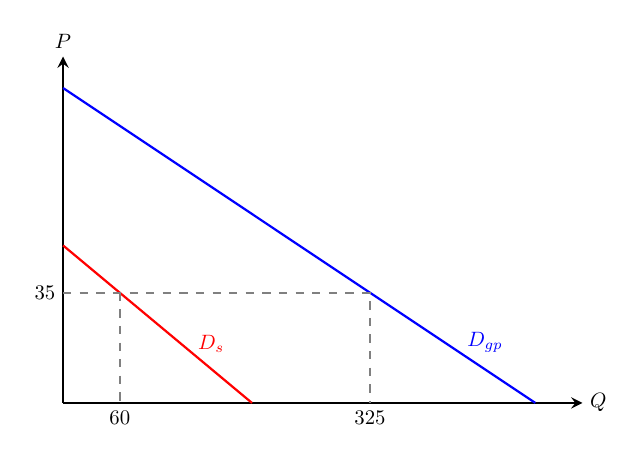
\begin{tikzpicture}[x=0.012cm, y=0.04cm, >=stealth, thick, every node/.style={scale=0.75}]
				\draw[->] (0,0) -- (550,0) node[right] {$Q$};
				\draw[->] (0,0) -- (0,110) node[above] {$P$};
				
				% 大众需求 P = 100 - 0.2Q
				\draw[blue] (0,100) -- (500,0) node[pos=0.85, above right, fill=white, inner sep=1pt] {$D_{gp}$};
				% 学生需求 P = 50 - 0.25Q
				\draw[red] (0,50) -- (200,0) node[pos=0.7, above right, fill=white, inner sep=1pt] {$D_s$};
				
				\draw[dashed, gray] (0,35) node[left, black] {$35$} -- (325,35) -- (325,0) node[below, black] {$325$};
				\draw[dashed, gray] (60,35) -- (60,0) node[below, black] {$60$};
			\end{tikzpicture}
		\end{center}
		
		b. 需求价格弹性计算
		
		根据需求点弹性的定义公式：
		$$ E_d = \frac{dQ}{dP} \cdot \frac{P}{Q} $$
		
		对于普通大众群体，在 $P=35$ 时的弹性为：
		$$ E_{d,gp} = (-5) \times \frac{35}{325} \approx -0.54 $$
		由于 $|E_{d,gp}| < 1$，说明该群体需求缺乏弹性。
		
		对于学生群体，在 $P=35$ 时的弹性为：
		$$ E_{d,s} = (-4) \times \frac{35}{60} \approx -2.33 $$
		由于 $|E_{d,s}| > 1$，说明该群体需求富有弹性。
		
		c. 收益最大化判定
		
		根据总收益与需求弹性的关系：
		$$ \frac{dTR}{dP} = Q(1 + E_d) $$
		当 $|E_d| < 1$ 时，价格与总收益同向变动，提价能增加收益；当 $|E_d| > 1$ 时，价格与总收益反向变动，降价能增加收益。
		目前普通大众缺乏弹性，应通过涨价增加收益；而学生群体富有弹性，应通过降价增加收益。因此，统一标价 35 美元并未实现总收益最大化。
		
		d. 总收益最大化定价
		
		方法一：边际收益法
		
		总收益最大化的必要条件是边际收益等于零，即：
		$$ MR = \frac{dTR}{dQ} = 0 $$
		
		对于普通大众，反需求函数为 $P = 100 - 0.2Q$，则：
		$$ TR_{gp} = 100Q - 0.2Q^2 $$
		$$ MR_{gp} = 100 - 0.4Q = 0 \implies Q^* = 250 $$
		代入需求函数得最优价格：
		$$ P_{gp}^* = 100 - 0.2 \times 250 = 50 $$
		
		对于学生群体，反需求函数为 $P = 50 - 0.25Q$，则：
		$$ TR_s = 50Q - 0.25Q^2 $$
		$$ MR_s = 50 - 0.5Q = 0 \implies Q^* = 100 $$
		代入需求函数得最优价格：
		$$ P_s^* = 50 - 0.25\times 100 = 25 $$
		
		方法二：二次函数最值法
		
		直接建立总收益关于价格 $P$ 的二次函数：
		$$ TR(P) = P \cdot Q(P) $$
		
		对于普通大众：
		$$ TR_{gp} = P(500 - 5P) = -5P^2 + 500P $$
		根据二次函数 $y = ax^2 + bx + c$ 的顶点公式 $x = -b/2a$，总收益最大化的价格为：
		$$ P_{gp}^* = \frac{-500}{2 \times (-5)} = 50 $$
		
		对于学生群体：
		$$ TR_s = P(200 - 4P) = -4P^2 + 200P $$
		总收益最大化的价格为：
		$$ P_s^* = \frac{-200}{2 \times (-4)} = 25 $$
		
		\begin{center}
			\begin{tikzpicture}[>=stealth, thick, every node/.style={scale=0.75}]
				% === 左图：普通大众 ===
				\begin{scope}[x=0.012cm, y=0.04cm]
					\draw[->] (0,0) -- (550,0) node[right] {$Q$};
					\draw[->] (0,0) -- (0,110) node[above] {$P, MR$};
					
					% 需求曲线与MR曲线
					\draw[blue] (0,100) -- (500,0) node[pos=0.9, above right] {$D_{gp}$};
					\draw[blue, dashed] (0,100) -- (250,0) node[below] {$100$};
					
					% 收益最大化点
					\draw[dashed, gray] (250,0) -- (250,50) -- (0,50) node[left, black] {$50$};
					\fill (250,50) circle (2pt) node[above right, fill=white, inner sep=1pt] {$E_1$};
					
					\node[below] at (250,-15) {(1) 普通大众 (最优 $P=50$)};
				\end{scope}
				
				% === 右图：学生群体 ===
				\begin{scope}[xshift=7.5cm, x=0.025cm, y=0.07cm]
					\draw[->] (0,0) -- (220,0) node[right] {$Q$};
					\draw[->] (0,0) -- (0,60) node[above] {$P, MR$};
					
					% 需求曲线与MR曲线
					\draw[red] (0,50) -- (200,0) node[pos=0.8, above right] {$D_s$};
					\draw[red, dashed] (0,50) -- (100,0) node[below] {$100$};
					
					% 收益最大化点
					\draw[dashed, gray] (100,0) -- (100,25) -- (0,25) node[left, black] {$25$};
					\fill (100,25) circle (2pt) node[above right, fill=white, inner sep=1pt] {$E_2$};
					
					\node[below] at (100,-8) {(2) 学生群体 (最优 $P=25$)};
				\end{scope}
			\end{tikzpicture}
		\end{center}
		
		
		\item \textbf{朱蒂已经决定每年不多不少花 500 美元在大学教材上，尽管她知道价格每年可能要上涨，并且她的祖父母明年将会给她一份可观的礼金。朱蒂对教材需求的价格弹性为多少？收入弹性呢？}
		
		\textbf{答：}
		1. 需求价格弹性分析：
		
		根据题意，朱蒂在教材上的总支出始终固定为 $P \cdot Q = 500$ 美元。由此可推导出她的教材需求函数为：
		$$Q = 500P^{-1}$$
		对该需求函数关于价格 $P$ 求导，得：
		$$\frac{dQ}{dP} = -500P^{-2}$$
		将其代入需求价格弹性公式 $E_d = \frac{dQ}{dP} \cdot \frac{P}{Q}$：
		$$E_d = \left( -500P^{-2} \right) \cdot \frac{P}{500/P} = -1$$
		朱蒂对教材的需求价格弹性恒等于 $-1$，属于单位弹性（Unit Elastic）。这意味着价格变动产生的支出效应完全被需求量的反向变动所抵消，总支出保持不变。
		
		2. 需求收入弹性分析：
		
		需求收入弹性定义为需求量变动百分比与收入变动百分比的比值。根据朱蒂的决策规则，无论其总收入 $I$（包括祖父母提供的礼金）如何变化，她分配给教材的预算始终固定为 500 美元。
		由于需求函数 $Q = 500/P$ 中不包含收入变量 $I$，即：
		$$\frac{\partial Q}{\partial I} = 0$$
		因此，需求收入弹性为：
		$$E_I = \frac{\partial Q}{\partial I} \cdot \frac{I}{Q} = 0$$
		朱蒂对教材的需求收入弹性为 $0$，说明教材在她的预算决策中表现为收入无弹性的商品。
		
		\begin{center}
			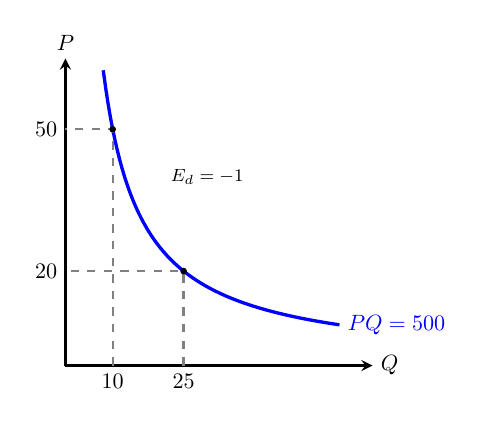
\begin{tikzpicture}[scale=0.6, >=stealth, thick, every node/.style={scale=0.8}, x=0.1cm, y=0.1cm]
				% 坐标轴
				\draw[->] (0,0) -- (65,0) node[right] {$Q$};
				\draw[->] (0,0) -- (0,65) node[above] {$P$};
				
				% 需求曲线 (PQ=500 -> P=500/Q)
				\draw[domain=8:58, samples=100, color=blue, very thick] plot (\x, {500/\x});
				\node[blue, right] at (58, 8.6) {$PQ=500$};
				
				% 选取两个点展示 TR 不变
				\draw[dashed, gray] (10,0) node[below, black] {$10$} -- (10,50) -- (0,50) node[left, black] {$50$};
				\draw[dashed, gray] (25,0) node[below, black] {$25$} -- (25,20) -- (0,20) node[left, black] {$20$};
				
				\fill (10,50) circle (2pt);
				\fill (25,20) circle (2pt);
				
				% 标注面积相等 (TR1 = TR2)
				\node[fill=white, inner sep=1pt] at (30,40) {\footnotesize $E_d = -1$};
			\end{tikzpicture}
		\end{center}
	
	\newpage
	\item \textbf{ACME公司确定，在目前的价格上，其计算机芯片的短期需求价格弹性为－2，其磁盘驱动器的短期需求价格弹性为－1。\\
		a. 如果公司决定将两种产品的价格都提高10％，其销售量会有什么变化？销售收入呢？\\
		b. 你能否从已知的信息中判断，哪个产品会给厂商带来最大的收入？如果能，为什么？如果不能，你还需要什么别的信息？}
	
	\textbf{答：}
	根据需求价格弹性定义及销售收入公式（$TR = P \times Q$），其核心计算关系如下：
	$$ \frac{\Delta Q}{Q} = E_d \times \frac{\Delta P}{P} $$
	$$ \frac{\Delta TR}{TR} = \left(1 + \frac{\Delta P}{P}\right)\left(1 + \frac{\Delta Q}{Q}\right) - 1 $$
	
	a. 当价格均提高10\%

		计算机芯片（$E_d = -2$）：
		$$ \frac{\Delta Q}{Q} = -2 \times 10\% = -20\% $$
		$$ \frac{\Delta TR}{TR} = (1+10\%)(1-20\%) - 1 = -12\% $$
		销量下降 20\%，销售收入下降 12\%。
		
		磁盘驱动器（$E_d = -1$）：
		$$ \frac{\Delta Q}{Q} = -1 \times 10\% = -10\% $$
		$$ \frac{\Delta TR}{TR} = (1+10\%)(1-10\%) - 1 = -1\% $$
		销量下降 10\%，销售收入下降 1\%。
	
	b. 不能判断。弹性信息仅反映价格变动对收入的边际影响（变动率），无法决定总收入的绝对水平。要比较两者总收入，还需获知两种产品的初始价格 $P$ 与初始销量 $Q$。
	
	\begin{center}
		\begin{tikzpicture}[scale=0.75, >=stealth, thick, every node/.style={scale=0.85}]
			% 坐标轴
			\draw[->] (0,0) -- (6.5,0) node[right] {$Q$};
			\draw[->] (0,0) -- (0,5) node[above] {$P$};
			
			% 需求曲线
			\draw[blue] (1,4.5) -- (5.5,1) node[right] {$D$};
			
			% 弹性区域划分虚线
			\draw[dashed, gray] (3.25, 2.75) -- (3.25, 0) node[below, black] {中点};
			
			% 标注产品与弹性
			\fill (2.125, 3.625) circle (2pt) node[above right, fill=white, inner sep=1pt] {芯片 $|E_d|>1$};
			\fill (3.25, 2.75) circle (2pt) node[above right, fill=white, inner sep=1pt] {驱动器 $|E_d|=1$};

		\end{tikzpicture}
	\end{center}
	\newpage
	\item \textbf{观察在下面概述的情形中一个人的行为，然后确定每一种商品相关的需求收入弹性（即该商品是正常品还是劣等品）。如果你不能确定收入弹性，你还需要别的什么信息？\\
		a. 比尔将其全部收入花在书籍和咖啡上。当他在书店的一只旧纸箱子里翻找东西时发现了20美元，他马上去买了一本新的精装诗集。\\
		b. 比尔丢失了他打算用来购买一杯双份蒸馏咖啡的10美元，他决定把新书折价卖给他的朋友，再用换来的钱买咖啡。\\
		c. 像波希米亚人那样生活已成了最新时尚，结果，咖啡和书籍的价格上涨了25％。比尔将这两种商品的消费削减了同样的百分比。\\
		d. 比尔离开了艺术学校，而获得了一个工商管理硕士（MBA）学位。他不喝咖啡且不读书了。现在他读《华尔街日报》，喝瓶装的矿泉水。}
	
	\textbf{答：}
	需求收入弹性
	$$E_I = \frac{\Delta Q/Q}{\Delta I/I}$$
	若 $E_I > 0$ 为正常品；若 $E_I < 0$ 为劣等品。
	
	a.书籍是正常品，咖啡的收入弹性无法确定。\\捡到20美元（意外的正向收入冲击）使他立即增加了书籍的消费，说明书籍的收入弹性为正，没有看出他对咖啡消费的改变，所以无法判断咖啡。
	
	b.书籍是正常品，咖啡是劣等品或者说必需品。\\丢失10美元是实际购买力的净损失（负向收入冲击)。在比尔的收入下降时，会卖掉新书（对书的需求下降），说明书籍是正常品；而他不惜卖书也要维持咖啡的消费，说明咖啡在收入下降时其需求未减反增，甚至优先维持），属于劣等品或者说必需品。
	
	c. 无法确定两者的收入弹性。\\这是价格同比例变动引发的价格效应（包含替代效应与收入效应），在未明确比尔名义收入是否发生变动以及变动幅度的情况下，无法分离出纯粹的收入弹性。
	
	d.咖啡和书籍是劣等品，《华尔街日报》和瓶装矿泉水是正常品。\\获得MBA学位通常伴随着收入的显著提升。当比尔的收入增加后，咖啡和书籍的需求直接降低到0，这说明其收入弹性为负，而对报纸和矿泉水的需求的增加说明其收入弹性为正。
	
	\item \textbf{假设食品需求的收入弹性是0.5，价格弹性是－1.0。假设费利西亚每年在食品上花费10000美元，食品价格为2美元，她的收入为25000美元。\\
		a. 如果一项食品销售税使得食品价格上升至2.5美元，她的食品消费会有什么变化？（提示：涉及较大价格变化时应假设采用弧弹性）\\
		b. 假设费利西亚得到2500美元的退税以缓解该销售税的影响。她现在的食品消费又将如何呢？\\
		c. 当她得到的退税数额等于销售税的支付数额时，她的境况是改善了还是变糟了？请说明原因。}
	
	\textbf{答：}
	初始食品消费量为：$Q_1 = 10,000 / 2 = 5,000$ 单位。
	
	a. 采用弧弹性公式计算价格上升后的消费量 $Q_2$：
	\[
	\begin{aligned}
		E_d &= \frac{\Delta Q / \bar{Q}}{\Delta P / \bar{P}} = \frac{Q_2 - 5000}{(5000 + Q_2)/2} / \frac{2.5 - 2.0}{(2.0 + 2.5)/2}
	\end{aligned}
	\]
	解得 $Q_2 = 4,000$ 单位。即食品消费量减少了 1,000 单位。
	
	b. 得到 2,500 美元退税后，收入变动率为 $\Delta I / I = 2,500 / 25,000 = 10\%$。
	根据需求收入弹性公式：
	\[
	\frac{\Delta Q}{Q} = E_I \cdot \frac{\Delta I}{I} = 0.5 \times 10\% = 5\%
	\]
	以 $Q_2$ 为基数计算，新的消费量为：$Q_3 = 4,000(1 + 5\%) = 4,200$ 单位。
	
	c. 费利西亚的境况变糟了。
	虽然退税能够在一定程度上弥补购买力的损失，但是销售税改变了食品和其他商品的相对价格，即使退税额等于其支付的税款，由于替代效应，消费者仍会减少对受税商品的消费并调整最优消费组合。根据显示偏好原理，退税后的新预算线虽经过或接近原来的点，但斜率已变化，消费者的最优选择点必然在无差异曲线下方区域。
	
	\begin{center}
		\begin{tikzpicture}[x=0.6cm, y=0.6cm, >=stealth, every node/.style={scale=0.8}]
			% 1. 坐标轴
			\draw[->, thick] (0,0) -- (15,0) node[right] {食品 $X$};
			\draw[->, thick] (0,0) -- (0,11) node[above] {其他商品 $Y$};
			
			% 2. 预算线逻辑计算 (采用夸大的退税截距以彻底分离曲线)：
			% L1 (初始): y = 8 - 4/7x 
			% L2 (征税): y = 8 - 1.25x (绕纵轴截距旋转，变得陡峭)
			% L3 (退税): y = 10 - 1.25x (平行外移，截距夸大至10以实现视觉分离)
			\draw[thick, black] (0,8) -- (14,0) node[pos=0.85, above right, inner sep=1pt] {$L_1$};
			\draw[thin, dashed, gray] (0,8) -- (6.4,0) node[pos=0.8, below left, inner sep=1pt] {$L_2$};
			\draw[thick, gray] (0,10) -- (8,0) node[pos=0.85, above left, inner sep=1pt, xshift=-4pt] {$L_3$};
			
			% 3. 无差异曲线绘制 (严格计算的一阶导数相切点坐标):
			% U0 (初始均衡): 与 L1 精确相切于 E0(7, 4), 系数 k = 28
			\draw[thick, blue, domain=2.8:13, samples=100] plot (\x, {28/\x}) node[right] {$U_0$};
			
			% U1 (最终均衡): 与 L3 精确相切于 E1(4, 5), 系数 k = 20
			\draw[thick, red, domain=2.0:9.5, samples=100] plot (\x, {20/\x}) node[right] {$U_1$};
			
			% 4. 均衡点标注 
			\filldraw[fill=white, draw=black, thick] (7,4) circle (1.5pt) node[above right, inner sep=2pt] {$E_0$};
			\filldraw[fill=white, draw=black, thick] (4,5) circle (1.5pt) node[above left, inner sep=2pt,yshift=-6pt,xshift=-3pt] {$E_1$};
			
			% 5. 辅助投影线与刻度标注
			\draw[dashed, gray] (7,0) node[below, black] {$5000$} -- (7,4);
			\draw[dashed, gray] (4,0) node[below, black, xshift=-4pt] {$4200$} -- (4,5);
			
		\end{tikzpicture}
	\end{center}
	
	\item \textbf{假设你经营着一个小企业，想预测你的产品价格提高之后需求量会发生什么变化。虽然你不知道你的产品的确切需求曲线，但是你知道第一年你要价45美元，销售了1200单位，第二年你要价30美元，销售了1800单位。\\
		a. 如果你打算把价格提高10％，那么，以百分比的形式计，对需求量变动的一个合理预测为多少？\\
		b. 如果你把价格提高10％，收入将会上升还是下降？}
	
	\textbf{答：}
	a. 首先运用弧弹性公式估算该区间的需求价格弹性：
	$$E_d = \frac{\Delta Q}{(Q_1+Q_2)/2} / \frac{\Delta P}{(P_1+P_2)/2} = -1$$
	由于价格提高 10\%，合理预测的需求量变动率为
	$$\frac{\Delta Q}{Q} = E_d \times 10\% = -10\%$$
	需求量将减少 10\%。
	
	b. 销售收入基本不变。由于该区间的需求弹性为单位弹性（$|E_d| = 1$），价格上升带来的正向边际收入与销量下降带来的负向边际损失刚好相互抵消。
	
	现价30美元，销量1800，初始收入 $TR = 54000$。提价10\%至33美元，销量下降10\%至1620，新收入 $TR = 33 \times 1620 = 53460$，两者差距极小。
	
	\newpage
	\item \textbf{假设你在管理一座营运成本基本上为零的收费桥梁。过桥需求 $Q$ 由 $P=15-(1/2)Q$ 给出。\\
		a. 画出过桥服务的需求曲线。\\
		b. 如果不收费，会有多少人通过该桥？\\
		c. 如果过桥费是5美元，相对应的消费者剩余的损失是多少？\\
		d. 该收费桥梁的运营方打算把价格提高到7美元。在这一相对较高的价格上，会有多少人通过该桥？该收费桥梁的收益是上升还是下降了？从你的答案出发，你对需求弹性有何判断？\\
		e. 求与价格从5美元上升到7美元相对应的消费者剩余的损失。}
	
	\textbf{答：}
	a. 需求曲线 $P = 15 - 0.5Q$ 是一条向下倾斜的直线，其纵轴截距为 15，横轴截距为 30,如下图所示）。
	
	b. 当不收费时（$P = 0$）：
	\[ 0 = 15 - 0.5Q \implies Q = 30 \]
	即会有 30 人通过该桥。
	
	c. 消费者剩余损失为两次价格水平下 $CS$ 的差值：
	\[ CS_0 (P=0) = \frac{1}{2} \times 30 \times 15 = 225 \]
	\[ CS_1 (P=5) = \frac{1}{2} \times 20 \times (15-5) = 100 \]
	\[ \Delta CS = 225 - 100 = 125 \text{ 美元} \]
	
	d. 当价格提高到 $P = 7$ 时，过桥人数 $Q = 2 \times (15 - 7) = 16$。
	收益变动分析如下：
	\[ TR_1 = 5 \times 20 = 100, \quad TR_2 = 7 \times 16 = 112 \]
	由于 $TR_2 > TR_1$，总收益上升。
	这表明在 $P \in [5, 7]$ 区间内，需求价格弹性 $|E_d| < 1$，即需求是缺乏弹性的，价格上涨带来的单位收益增加超过了销量下降的损失。
	
	e. 价格从 5 美元上升到 7 美元对应的消费者剩余损失为：
	\[ CS_2 (P=7) = \frac{1}{2} \times 16 \times (15-7) = 64 \]
	\[ \text{损失} = CS_1 - CS_2 = 100 - 64 = 36 \text{ 美元} \]
	
	\begin{center}
		\begin{tikzpicture}[scale=0.7, >=stealth, thick, every node/.style={scale=0.85}]
			% --- 左图：P=0 到 P=5 的变动 ---
			\begin{scope}[xshift=0cm]
				\draw[->] (0,0) -- (6.5,0) node[right] {$Q$};
				\draw[->] (0,0) -- (0,5.5) node[above] {$P$};
				
				% 需求曲线 (x=Q/5, y=P/3)
				\draw[blue] (0,5) node[left, black] {15} -- (6,0) node[below, black] {30};
				
				% P=5 辅助线
				\draw[dashed, gray] (0,1.67) node[left, black] {5} -- (4,1.67) -- (4,0) node[below, black] {20};
				
				% CS损失区域 (梯形 0,0, 4,1.67, 6,0)
				\fill[red, fill opacity=0.2] (0,0) -- (0,1.67) -- (4,1.67) -- (6,0) -- cycle;
				\node[red!80!black, fill=white, inner sep=1pt] at (2,0.8) {$\Delta CS = 125$};
				\node[below] at (3,-0.8) {(1) $P=0 \to 5$ 时的福利损失};
			\end{scope}
			
			% --- 右图：P=5 到 P=7 的变动 ---
			\begin{scope}[xshift=8.5cm]
				\draw[->] (0,0) -- (6.5,0) node[right] {$Q$};
				\draw[->] (0,0) -- (0,5.5) node[above] {$P$};
				
				\draw[blue] (0,5) node[left, black] {15} -- (6,0) node[below, black] {30};
				
				% P=5 辅助线
				\draw[dashed, gray] (0,1.67) node[left, black, xshift=-2pt] {5} -- (4,1.67) -- (4,0) node[below, black] {20};
				% P=7 辅助线
				\draw[dashed, gray] (0,2.33) node[left, black, xshift=-2pt] {7} -- (3.2,2.33) -- (3.2,0) node[below, black] {16};
				
				% CS损失区域 (梯形 0,1.67, 0,2.33, 3.2,2.33, 4,1.67)
				\fill[orange, fill opacity=0.3] (0,1.67) -- (0,2.33) -- (3.2,2.33) -- (4,1.67) -- cycle;
				\node[orange!80!black, fill=white, inner sep=1pt] at (1.6,2) {损失 $= 36$};
				\node[below] at (3,-0.8) {(2) $P=5 \to 7$ 时的福利损失};
			\end{scope}
		\end{tikzpicture}
	\end{center}
	
	\newpage
	\item \textbf{维拉正打算升级她那台新的个人计算机上的操作系统。她听说新操作系统Linux在技术上优于Windows而且价格低很多。然而，在询问了她的朋友之后，她发现他们用的都是装了Windows的个人计算机。他们也认为Linux的拷贝相对较少。维拉选择了Windows。你能解释一下她的决定吗？}
	
	\textbf{答：}
	维拉的决定是正网络外部性（连带外部效应或攀比效应）的典型体现。一个消费者如果需求随着其他人购买该商品数量增加而相应地增多时，那么就存在正的网络外部性。尽管Linux具有技术和价格上的内生优势，但操作系统核心效用更依赖于市场的大规模用户基数，由于维拉的朋友及广大市场都在广泛使用Windows，这种庞大的网络不仅提供了直接的文件兼容、社交等便利，还构筑起远超Linux丰富应用软件和硬件支持；反之则必须独自面对极高的学习成本以及软件缺失造成的隐形折损。因此，Windows巨大的正向网络外部性收益远远超出了Linux价格和技术上的优势，这也是维拉做出最终决策的根本原因。
	
	\item \textbf{假设你是一个农业合作组织的顾问，该组织正在决定其成员明年要不要将他们的棉花生产减半。该组织需要你的建议，即这个决定是否将会提高其成员的收益。了解到棉花（$C$）与大豆（$S$）的种植面积在南方是竞争性的，你对棉花需求的估计为 $C=3.5-1.0P_C+0.25P_S+0.50I$，这里 $P_C$ 为棉花的价格，$P_S$ 为大豆的价格，$I$ 为收入。你是该支持还是反对这项计划？是否需要更多的信息以使你能够做出确切的回答？}
	
	\textbf{答：}
	不能直接得出支持或反对的结论，需要更多的核心市场信息。判定减产能否提高总收益，其核心在于评估棉花的需求价格弹性。如果棉花需求缺乏弹性，即 $|E_d| < 1$，则减产导致的价格涨幅将超过产量的跌幅，从而增加总收益；反之，若需求富有弹性，减产会使总收益锐减。
	
	给定的需求函数仅仅提供了需求曲线的斜率系数 
	$$\frac{\partial C}{\partial P_C} = -1.0$$
	根据点弹性公式：
	$$ E_d = \frac{\partial C}{\partial P_C} \cdot \frac{P_C}{C} = -1.0 \times \frac{P_C}{C} $$
	要计算具体的弹性值并做出确切回答，我们必须另外获得以下信息：一是当期大豆的市场价格$P_S$和宏观收入水平$I$，这用来测算基期棉花实际需求量$C$和市场均衡价格$P_C$；二是其他独立棉花产区供给反应预期。如果其它独立棉花产区不减产甚至增加产量填补空缺，合作社单边减产也没有办法推高市场价格$P_C$，最终只会失去市场份额、导致损失利润。
	
	\newpage
	\item \textbf{一个消费者只吃牛排和土豆。其预算为每10天30美元，而她必须买足够的土豆来吃，至少每天2单位。\\
		a. 土豆价格为0.5美元，牛排价格为10美元。消费者将消费两种商品各多少？\\
		b. 现在假设土豆的价格上升为1美元。消费者购买每种商品各多少？\\
		c. 现在假设土豆价格上升为1.25美元。消费者购买每种商品各多少？\\
		d. 土豆是哪种商品？\\
		e. 你预测土豆的需求曲线会一直保持这种趋势吗？为什么？}
	
	\textbf{答：}
	设消费的土豆数量为 $X$，牛排数量为 $Y$。消费者的预算约束为 $P_X X + P_Y Y = 30$。维持生存的极值约束为 $X \ge 20$（即 10 天至少消费 20 单位土豆）。
	
	a. 当 $P_X = 0.5, P_Y = 10$ 时。
	维持生存至少需购买 20 单位土豆，花费 $20 \times 0.5 = 10$ 美元。剩余 20 美元预算恰好可购买 2 单位牛排。因此，消费组合为 20 单位土豆，2 单位牛排。
	
	b. 当 $P_X = 1$ 时。
	维持生存至少需购买 20 单位土豆，花费 $20 \times 1 = 20$ 美元。剩余 10 美元预算恰好可购买 1 单位牛排。因此，消费组合为 20 单位土豆，1 单位牛排。
	
	c. 当 $P_X = 1.25$ 时。
	维持生存的 20 单位土豆需花费 $20 \times 1.25 = 25$ 美元。剩余 5 美元不足以购买 1 单位的完整牛排。由于牛排不可细分，为了满足生存需要并耗尽预算，所有的资金将被迫全部投入土豆的购买中：
	$$ X = \frac{30}{1.25} = 24 $$
	因此，消费组合为 24 单位土豆，0 单位牛排。
	
	d. 土豆是吉芬品。当土豆价格从 1 美元升至 1.25 美元时，预算空间的极度压缩产生了巨大的负向收入效应。由于必须满足绝对的生存线限制，消费者被迫放弃了昂贵的肉类，转而增加了对廉价主食（土豆）的需求量（从 20 增至 24）。这表现出了“价格上升，需求量反而增加”的违背需求法则的典型特征。
	
	e. 不会一直保持这种趋势。一旦土豆价格超过 1.5 美元（此时 30 美元的总预算全部用于买土豆也无法达到 20 单位的最低生存线），预算约束将彻底崩塌。为了生存，消费者将被迫放弃现有的消费组合体系，去寻找更廉价的替代主食，此时土豆的需求量必然急剧下降。
	
	\begin{center}
		\begin{tikzpicture}[x=0.3cm, y=1.2cm, >=stealth, thick, every node/.style={scale=0.85}]
			% 1. 坐标轴
			\draw[->] (0,0) -- (32,0) node[right] {土豆 $X$};
			\draw[->] (0,0) -- (0,3.6) node[above] {牛排 $Y$};
			
			% 纵轴截距
			\node[left] at (0,3) {$3$};
			
			% 2. 最低消费生存线 (移到底层，颜色调淡，避免喧宾夺主)
			\draw[dashed, red!50, very thick] (20,0) -- (20,3.3) 
			node[above, red!80!black] {$X \ge 20$};
			
			% 3. 预算线演变 (错开标签位置，彻底消除重叠)
			% 预算线 1 (P_x = 0.5) - 浅灰，标签放末端
			\draw[gray] (0,3) -- (28, 1.6) node[right] {$P_X=0.5$};
			
			% 预算线 2 (P_x = 1.0) - 深灰，标签放末端
			\draw[darkgray] (0,3) -- (30, 0) node[above right] {$P_X=1.0$};
			
			% 预算线 3 (P_x = 1.25) - 主题蓝，标签放线段中下部开阔处
			\draw[blue] (0,3) -- (24, 0);
			\node[blue, below left,yshift=3pt] at (14, 1.25) {$P_X=1.25$};
			
			% 4. 投影虚线 (细化线条，精简文字)
			\draw[dashed, gray, thin] (0,2) node[left, black] {$2$} -- (20,2);
			\draw[dashed, gray, thin] (0,1) node[left, black] {$1$} -- (20,1);
			
			% X轴关键刻度
			\draw (20,0) -- (20,-0.1) node[below] {$20$};
			\draw (24,0) -- (24,-0.1) node[below] {$24$};
			
			% 5. 均衡点 (仅保留代号，坐标已由坐标轴自然体现)
			\fill[gray] (20,2) circle (2pt) node[above right] {$E_1$};
			\fill[darkgray] (20,1) circle (2pt) node[above right] {$E_2$};
			\fill[blue] (24,0) circle (2pt) node[above right] {$E_3$};
			
			% 6. 吉芬效应指示 (移至横轴下方，彻底解决画面内部拥挤)
			\draw[->, red, thick] (20.5, -0.5) -- (23.5, -0.5) node[midway, below] {吉芬效应};
		\end{tikzpicture}
	\end{center}
	
	\end{enumerate}
	
	\newpage
	\section{附录练习题}
	\begin{enumerate}[label=\textbf{\arabic*.}, leftmargin=*]
		\item \textbf{下面的效用函数中哪些符合凸的无差异曲线？哪些并不符合？}\\
			a. \( U(X,Y) = 2X + 5Y \)\\
			b. \( U(X,Y) = (XY)^{0.5} \)\\
			c. \( U(X,Y) = \min(X,Y) \)，这里 $\min$ 为 $X$ 和 $Y$ 两个数值中的最小值。\\
			d. \( U(X,Y) = \log(X) + \log(Y) \)
		
		\textbf{答：}
		无差异曲线凸性的定义：偏好是凸的，当且仅当任意两个无差异消费束的加权平均至少与原消费束一样好。其中，边际替代率（$MRS$）严格递减对应严格凸，$MRS$ 非递增对应弱凸。
		
		\begin{enumerate}[label=\textbf{\alph*.}, leftmargin=2em]
			\item $U(X,Y) = 2X + 5Y$：完全替代型效用函数，无差异曲线为直线，$MRS=MU_X/MU_Y=0.4$（恒定不变），属于弱凸。
			\item $U(X,Y) = (XY)^{0.5}$：柯布-道格拉斯效用函数，$MRS=Y/X$（随 $X$ 增加严格递减），无差异曲线凸向原点，属于严格凸。
			\item $U(X,Y) = \min(X,Y)$：完全互补型效用函数，无差异曲线为 L 形，两种商品必须按固定比例消费，不存在替代关系，属于弱凸。
			\item $U(X,Y) = \log(X) + \log(Y) = \log(XY)$：这是柯布-道格拉斯效用函数的严格单调递增变换，与 (b) 代表完全相同的偏好，$MRS=Y/X$ 严格递减，无差异曲线同样凸向原点，属于严格凸。
		\end{enumerate}
		
		\begin{center}
			\begin{tikzpicture}[scale=0.75, >=stealth, thick, every node/.style={scale=0.85}]
				% 完全替代 (a)
				\begin{scope}[xshift=0cm]
					\draw[->] (0,0) -- (4,0) node[right] {$X$};
					\draw[->] (0,0) -- (0,4) node[above] {$Y$};
					\draw[blue] (0.5, 3.0) -- (3.5, 1.2) node[right, fill=white, inner sep=1pt] {$U$};
					\node[below] at (2,-0.5) {(a) 弱凸 (直线)};
				\end{scope}
				% 柯布-道格拉斯 (b)(d)
				\begin{scope}[xshift=5.8cm]
					\draw[->] (0,0) -- (4,0) node[right] {$X$};
					\draw[->] (0,0) -- (0,4) node[above] {$Y$};
					\draw[red, domain=0.6:3.5, samples=100] plot (\x, {2.1/\x}) node[right, fill=white, inner sep=1pt] {$U$};
					\node[below] at (2,-0.5) {(b)(d) 严格凸 (双曲线)};
				\end{scope}
				% 完全互补 (c)
				\begin{scope}[xshift=11.6cm]
					\draw[->] (0,0) -- (4,0) node[right] {$X$};
					\draw[->] (0,0) -- (0,4) node[above] {$Y$};
					\draw[green!60!black] (1.8, 3.5) -- (1.8, 1.8) -- (3.5, 1.8) node[right, fill=white, inner sep=1pt] {$U$};
					\draw[dashed, gray] (0,0) -- (1.8, 1.8);
					\node[below] at (2,-0.5) {(c) 弱凸 (L形)};
				\end{scope}
			\end{tikzpicture}
		\end{center}
		
		\item \textbf{说明下面两个效用函数所导出的商品 $X$ 和 $Y$ 的需求函数相同。\\
			a. \( U(X,Y) = \log(X) + \log(Y) \)\\
			b. \( U(X,Y) = (XY)^{0.5} \)}
		
		\textbf{答：}
		正单调变换不改变消费者的序数偏好，因此得出的最优消费选择与需求函数完全一致。设商品价格为 $P_X, P_Y$，收入为 $I$，预算约束为 $P_X X + P_Y Y = I$。
		
		\textbf{a. $U(X,Y) = \log(X) + \log(Y) = \log(XY)$}
		
		消费者效用最大化的一阶条件为边际效用之比等于价格之比：
		$$\frac{MU_X}{MU_Y} = \frac{Y}{X} = \frac{P_X}{P_Y} \implies Y = \frac{P_X}{P_Y}X$$
		代入预算约束方程：
		$$P_X X + P_Y \left( \frac{P_X}{P_Y}X \right) = I \implies 2P_X X = I$$
		解得需求函数为：
		$$X^* = \frac{I}{2P_X}, \quad Y^* = \frac{I}{2P_Y}$$
		
		\textbf{b. $U(X,Y) = (XY)^{0.5}$}
		
		同样根据一阶条件求解：
		$$\frac{MU_X}{MU_Y} = \frac{0.5X^{-0.5}Y^{0.5}}{0.5X^{0.5}Y^{-0.5}} = \frac{Y}{X} = \frac{P_X}{P_Y} \implies Y = \frac{P_X}{P_Y}X$$
		由于边际替代率与 (a) 完全相同，代入预算约束后得到的需求函数也完全一致：
		$$X^* = \frac{I}{2P_X}, \quad Y^* = \frac{I}{2P_Y}$$
		
		\item \textbf{假设效用函数由 $U(X,Y) = \min(X,Y)$ 给出，正如练习题1中的c部分所示。那么将因为 $X$ 价格的变化而引起的其需求的变化进行分解的斯卢茨基方程是什么？什么是收入效应？什么是替代效应？}
		
		\textbf{答：}
		对于完全互补品 $U(X,Y) = \min(X,Y)$，消费者的最优选择始终满足固定比例消费，即 $X = Y$。结合预算约束方程 $P_X X + P_Y Y = I$，可推导出该商品的初始需求函数为：
		$$X = \frac{I}{P_X + P_Y}$$
		
		斯卢茨基方程的一般形式将价格变动引起的总效应精确分解为替代效应和收入效应两部分：
		$$ \underbrace{\frac{\partial X}{\partial P_X}}_{\text{总效应}} = \underbrace{\left. \frac{\partial X}{\partial P_X} \right|_{\bar{U}}}_{\text{替代效应}} + \underbrace{\left( -X \frac{\partial X}{\partial I} \right)}_{\text{收入效应}} $$
		
		针对完全互补品：
		
		替代效应：由于商品必须按固定比例消费，无差异曲线呈现为直角 L 型。当相对价格发生变化时，如果对消费者进行收入补偿以维持其原有效用水平，其最优消费组合依然被死死锁定在无差异曲线的直角拐点上，不存在两种商品之间的相互替代。因此，完全互补品的替代效应恒等于 $0$，即
		$$\left. \frac{\partial X}{\partial P_X} \right|_{\bar{U}} = 0$$
		
		收入效应：既然替代效应为零，价格的变化便仅仅通过改变消费者的实际购买力来影响需求。当 $X$ 的价格发生变化时，引起的实际收入变动带来的收入效应计算如下：
		$$ -X \frac{\partial X}{\partial I} = -X \left( \frac{1}{P_X + P_Y} \right) = - \frac{I}{(P_X + P_Y)^2} $$
		
		总效应：价格变化带来的总效应完全由收入效应构成。对需求函数直接求导也可印证此结论：
		$$ \frac{\partial X}{\partial P_X} = - \frac{I}{(P_X + P_Y)^2} $$
		
		这说明，对于完全互补品而言，其斯卢茨基方程退化并简化为总效应完全等于收入效应：
		$$ \frac{\partial X}{\partial P_X} = -X \frac{\partial X}{\partial I} $$
		
		\begin{center}
			\begin{tikzpicture}[x=0.8cm, y=0.8cm, >=stealth, thick, every node/.style={scale=0.85}]
				% 坐标轴
				\draw[->] (0,0) -- (9.5,0) node[right] {$X$};
				\draw[->] (0,0) -- (0,8.5) node[above] {$Y$};
				
				% 比例射线 X=Y
				\draw[dashed, gray] (0,0) -- (7.5,7.5);
				
				% 预算线 BL1
				\draw[black] (0,6) node[left] {$BL_1$} -- (9, 1.5) node[right] {$BL_1$}; 
				
				% 预算线 BL2 (X价格上升)
				\draw[blue] (0,6) -- (6,0) node[below] {$BL_2$};
				
				% 斯卢茨基补偿预算线 BLC (经过 E1，平行于 BL2)
				\draw[red, dashed] (0,8) node[left] {$BL_C$} -- (8,0) node[below] {$BL_C$};
				
				% L型无差异曲线
				\draw[thick, blue] (3,6.5) -- (3,3) -- (6.5,3) node[right] {$U_2$};
				\draw[thick, blue] (4,7.5) -- (4,4) -- (7.5,4) node[right] {$U_1$};
				
				% 均衡点 (使用 fill=white 防止遮挡网格与连线)
				\fill[black] (4,4) circle (2pt) node[above right, fill=white, inner sep=1pt,yshift=2pt,xshift=2pt] {$E_1 (E_C)$};
				\fill[black] (3,3) circle (2pt) node[below right, fill=white, inner sep=1pt,yshift=-3pt] {$E_2$};
				
				% 投影线与标注
				\draw[dashed, gray] (4,0) node[below, black] {$X_1$} -- (4,4);
				\draw[dashed, gray] (3,0) node[below, black] {$X_2$} -- (3,3);
				
				% 效应箭头
				\draw[->, purple, very thick] (3.8, -0.6) -- (3.2, -0.6) node[midway, below] {收入效应 = 总效应};
				\node[below, text=black] at (3.5, -1.3) {(替代效应 $= 0$)};
			\end{tikzpicture}
		\end{center}
		
		\item \textbf{莎伦的效用函数如下：$U(X,Y) = \sqrt{X} + \sqrt{Y}$。其中，$X$ 为她对单独包装的块状糖的消费量，价格 $P_X = 1$ 美元，$Y$ 为浓咖啡的消费量，价格 $P_Y = 3$ 美元。\\
			a. 推导莎伦对单独包装的块状糖和浓咖啡的需求函数。\\
			b. 假定她的收入 $I = 100$ 美元。莎伦将消费多少数量的单独包装的块状糖和浓咖啡？\\
			c. 收入的边际效用为多少？}
		
		\textbf{答：}
		
		\textbf{a. 推导需求函数}
		
		消费者预算约束为 $P_X X + P_Y Y = I$。分别计算商品的边际效用：
		$$MU_X = \frac{1}{2\sqrt{X}}, \quad MU_Y = \frac{1}{2\sqrt{Y}}$$
		根据效用最大化条件，边际效用之比等于价格之比：
		$$\frac{MU_X}{MU_Y} = \frac{\sqrt{Y}}{\sqrt{X}} = \frac{P_X}{P_Y} \implies \frac{Y}{X} = \left(\frac{P_X}{P_Y}\right)^2 \implies Y = \left(\frac{P_X}{P_Y}\right)^2 X$$
		代入预算约束方程中：
		$$P_X X + P_Y \left(\frac{P_X}{P_Y}\right)^2 X = I \implies X \left( P_X + \frac{P_X^2}{P_Y} \right) = I$$
		由此解得广义需求函数为：
		$$X^* = \frac{I}{P_X + P_X^2/P_Y}, \quad Y^* = \frac{I}{P_Y + P_Y^2/P_X}$$
		将已知的 $P_X = 1$ 和 $P_Y = 3$ 代入，得到具体的线性需求函数形式：
		$$X^* = \frac{I}{1 + 1/3} = \frac{3I}{4}, \quad Y^* = \frac{I}{3 + 9} = \frac{I}{12}$$
		
		\newpage
		\textbf{b. 计算具体消费量}
		
		将收入 $I = 100$ 美元代入推导出的需求函数中：
		$$X^* = \frac{3 \times 100}{4} = 75, \quad Y^* = \frac{100}{12} \approx 8.33$$
		即莎伦将消费 $75$ 块块状糖和约 $8.33$ 杯浓咖啡。
		
		\textbf{c. 计算收入的边际效用}
		
		收入的边际效用等于拉格朗日乘数 $\lambda$，根据一阶条件 
		$$\lambda = \frac{MU_X}{P_X}$$
		代入最优解进行计算：
		$$\lambda = \frac{1}{2P_X\sqrt{X^*}} \approx 0.0577$$
		这表明，在当前消费水平下，每增加 $1$ 美元的收入，莎伦的总效用将增加约 $0.0577$ 个单位。
		
		\item \textbf{莫里斯的效用函数如下：$U(X,Y) = 20X + 80Y - X^2 - 2Y^2$。其中，$X$ 为他对 CD 的消费量，价格为 1 美元，$Y$ 为他对录像带的消费量，租金价格为 2 美元。他计划在这两种形式的娱乐上花 41 美元。求最大化莫里斯效用的 CD 数量与录像带租赁数量。}
		
		\textbf{答：}
		根据题意，莫里斯的预算约束方程为 $X + 2Y = 41$。分别计算两种商品的边际效用：
		$$MU_X = 20 - 2X, \quad MU_Y = 80 - 4Y$$
		
		根据效用最大化条件，边际效用之比等于价格之比：
		$$\frac{MU_X}{MU_Y} = \frac{P_X}{P_Y} \implies \frac{20 - 2X}{80 - 4Y} = \frac{1}{2}$$
		化简得：$Y = X + 10$
		
		将 $Y = X + 10$ 联立代入预算约束方程：
		$$X + 2(X + 10) = 41 \implies X^* = 7$$
		$$Y^* = 7 + 10 = 17$$
		
		此时莫里斯的最大总效用为：
		$$U(7,17) = 20 \times 7 + 80 \times 17 - 7^2 - 2 \times 17^2) = 873$$
		
		\begin{center}
			\begin{tikzpicture}[x=0.4cm, y=0.2cm, >=stealth, thick, every node/.style={scale=0.85}]
				% 1. 坐标轴 (物理长宽比严格 1:1，呈现完美的方形包围盒)
				\draw[->] (0,0) -- (12,0) node[right] {$X$};
				\draw[->] (0,0) -- (0,24) node[above] {$Y$};
				\node[below left] at (0,0) {$O$};
				
				% 2. 预算线 BL: 只画到正方形边界 (X=11.5处)
				\draw[black] (0, 20.5) -- (11.5, 14.75);
				\fill[black] (0, 20.5) circle (1.5pt) node[left] {$20.5$};
				
				% 3. 无差异曲线 U=873
				\draw[blue!80, domain=4.9:11.5, samples=100, smooth] 
				plot (\x, {20 - sqrt(13.5 - 0.5*(\x-10)^2)}) 
				node[below right, font=\footnotesize] {$U=873$};
				
				% 4. 均衡点 E 与投影辅助线
				\coordinate (E) at (7, 17);
				\draw[dashed, gray!70, thin] (7,0) node[below, text=black] {$7$} -- (E) 
				-- (0,17) node[left, text=black] {$17$};
				\fill[red] (E) circle (1.5pt);
				
				% 5. 核心标签
				\node[above right, text=red, fill=white, inner sep=1pt, xshift=1pt, yshift=1pt] at (E) {$E(7,17)$};
			\end{tikzpicture}
		\end{center}
		
	\end{enumerate}
	% =======================================================
	%               第 5 章：不确定性与消费者行为
	% =======================================================
	\chapter{不确定性与消费者行为}
	
	\section{复习题}
	\begin{enumerate}[label=\textbf{\arabic*.}, leftmargin=*]
		\item \textbf{如果一个人是风险厌恶者，这意味着什么？为什么有些人厌恶风险，而有些人又喜好风险？}
		
		\textbf{答：}
		风险厌恶者是指在面临期望收益相同的确定性方案和不确定性方案时，总是偏好确定性结果。从效用函数来看，其效用函数具有严格凹性（边际效用递减），也就是说增加财富带来的边际效用减损小于减少财富所引起的效用变化。
		
		偏好差异的根源在于每个人的效用函数不同。风险厌恶者面对递减的边际效用。而风险喜好者却会拥有递增的边际效用（效用函数为凸）。这些差异由各种因素决定：一是极度贫困或极度富有都可能改变个体的风险边际偏好；二是心理感知，个人对损失的敏感程度（损失厌恶）不同；三是社会背景、职业特征等会造成不同的期望效用评估框架。
		
		\item \textbf{在对可变性的度量中，为什么方差比取值范围更好？}
		
		\textbf{答：}
		取值范围仅关注分布的两个极端点（最大值与最小值），完全忽略了所有中间结果及其发生的概率分布。若两个方案极值相同但其中一个结果更向均值集中，取值范围将无法区分其风险差异。
		
		方差通过计算所有可能结果与期望值偏离程度的平方，并以概率为权重进行加权平均，全面捕捉了概率分布的离散程度。它不仅考虑了变动的幅度，更考量了变动的频率，因此能够更科学、精准地衡量经济活动的风险（可变性）。
		\begin{center}
			\begin{tikzpicture}[x=0.6cm, y=1.2cm, >=stealth, thick, every node/.style={scale=0.85}]
				% 坐标轴
				\draw[->] (0,0) -- (10.5,0) node[right] {结果 ($X$)};
				\draw[->] (0,0) -- (0,3.6) node[above] {概率密度};
				
				% 绘制两条曲线 (使用 cos 函数的幂次来确保在 x=1 和 x=9 时完美收敛于 0)
				% 曲线A：方差小，集中 (8次幂使其陡峭)
				\draw[blue, thick, domain=1:9, samples=100] plot (\x, {3 * (cos((\x-5)*22.5))^8});
				
				% 曲线B：方差大，分散 (2次幂使其平缓)
				\draw[gray, thick, dashed, domain=1:9, samples=100] plot (\x, {1.4 * (cos((\x-5)*22.5))^2});
				
				% 均值辅助线
				\draw[dashed, thin, gray] (5,0) node[below, text=black] {$E[X]$} -- (5,3.2);
				
				% 边界辅助线 (极值点)
				\draw[dashed, thin, gray] (1,0) node[below, text=black] {$X_{\min}$} -- (1,0.6);
				\draw[dashed, thin, gray] (9,0) node[below, text=black] {$X_{\max}$} -- (9,0.6);
				
				% 标注曲线A (带白色背景防遮挡)
				\draw[->, thin, blue] (3.2, 2.8) node[above, fill=white, inner sep=1pt,xshift=-6pt] {方案 A: 方差小} to[bend left=15] (4.3, 2.1);
				
				% 标注曲线B (带白色背景防遮挡)
				\draw[->, thin, gray!90!black] (7.5, 1.8) node[above, fill=white, inner sep=1pt,xshift=5pt] {方案 B: 方差大} to[bend right=15] (6.6, 1.1);
				
				% 底部大括号表示“相同的取值范围”
				\draw[decorate, decoration={brace, amplitude=5pt, mirror}, black, thin] (1, -0.6) -- (9, -0.6) node[midway, below=5pt] {相同的取值范围};
			\end{tikzpicture}
		\end{center}
		\item \textbf{乔治有5000美元可以投资于共同基金。共同基金 A 的期望回报率为 15\%，共同基金 B 的期望回报率为 10\%。乔治应该选择共同基金 A 还是 B？}
		
		\textbf{答：}
		仅凭期望回报率无法进行理性决策。决策取决于乔治的风险偏好以及两只基金的风险水平（标准差）。
		
		若乔治为风险厌恶者，且基金 A 的风险显著高于基金 B，他可能会选择回报率较低但更稳健的基金 B。乔治的最优决策取决于他的无差异曲线与风险-收益预算线的切点。在未获得基金风险参数（标准差）和乔治风险系数的情况下，无法判定最终选择。
		
		\item \textbf{消费者追求期望效用最大化的含义是什么？你能举出某个人不追求期望效用最大化的例子吗？}
		
		\textbf{答：}
		期望效用最大化的核心含义是：消费者在不确定环境下做决策时，其目标不是追求“金钱数额”的平均值最大化，而是追求“金钱带来的满足感（效用）”的加权平均值最大化。
		由于边际效用递减，风险厌恶者会拒绝一个期望收益为正但风险极大的方案。例如，相对于 50\% 概率获得 2000 元、50\% 概率获得 0 元（期望收益 1000 元）的赌局，消费者往往更偏好稳拿 1000 元，因为后者提供的确定性满足感更高。
		
		在面临收益时，面对“100\% 确定获得 3000 元”与“80\% 概率获得 4000 元（期望收益 3200 元）”，多数人会放弃高期望收益而选择前者，表现出对确定性的强烈偏好（风险厌恶）；\\
		但在面临同等条件的损失时，面对“100\% 确定损失 3000 元”与“80\% 概率损失 4000 元（期望损失 3200 元）”，多数人却会拒绝确定性损失，选择去赌那个概率，表现出风险爱好。
		
		这种“面对收益求稳、面对损失搏命”的偏好，证明了个体决策并非始终遵循期望效用最大化。
		
		\item \textbf{为什么有时即使支付的保险费超过了期望损失，人们通常还是想要得到对风险环境的完全保险？}
		
		\textbf{答：}
		由于风险厌恶者的效用函数是凹的，遭受损失时的效用大幅下降远超同额保费带来的效用减损。支付略高于期望损失的保费，可以换取一种“确定性的效用”，其水平高于承担风险时的“期望效用”。期望财富与确定性等值（CE）之间的差额即为风险溢价。只要保费中的管理费（附加保费）小于风险溢价，完全保险就是理性的。
		
		\begin{center}
			\begin{tikzpicture}[x=0.3cm, y=1.2cm, >=stealth, thick, every node/.style={scale=0.8}]
				% 坐标轴
				\draw[->] (0,0) -- (22,0) node[right] {财富 ($W$)};
				\draw[->] (0,0) -- (0,4.8) node[above] {效用 ($U$)};
				
				% 设定参数: W1=2, W2=18 -> E[W]=10. U=sqrt(x)
				% U(2)=1.41, U(18)=4.24, E[U]=2.825. CE = 2.825^2 = 7.98
				
				% 效用曲线 (去除 ultra thick, 保持小图精致感)
				\draw[blue, thick, domain=0:20, samples=100] plot (\x, {sqrt(\x)}) node[right] {$U(W)$};
				
				% 弦 (期望效用线)
				\draw[red, dashed, thick] (2,1.414) -- (18,4.242);
				
				% 关键点投影 (使用 thin 避免辅助线喧宾夺主)
				\draw[dashed, gray, thin] (2,1.414) -- (2,0) node[below, black] {$W_1$};
				\draw[dashed, gray, thin] (2,1.414) -- (0,1.414) node[left, black] {$U(W_1)$};
				
				\draw[dashed, gray, thin] (18,4.242) -- (18,0) node[below, black] {$W_2$};
				\draw[dashed, gray, thin] (18,4.242) -- (0,4.242) node[left, black] {$U(W_2)$};
				
				% E[W] 与 U(E[W])
				\draw[dashed, gray, thin] (10,3.162) -- (10,0) node[below, black] {$E[W]$};
				\draw[dashed, gray, thin] (10,3.162) -- (0,3.162) node[left, black] {$U(E[W])$};
				\fill (10,3.162) circle (1.5pt);
				
				% E[U] 与 CE
				\draw[dashed, gray, thin] (7.98,2.828) -- (7.98,0) node[below, black] {$CE$};
				\draw[dashed, gray, thin] (0,2.828) node[left, black] {$E[U]$} -- (10,2.828);
				
				% E[U] 在弦上的点 A (微调 label 位置防遮挡)
				\fill (10,2.828) circle (1.5pt) node[below right, xshift=1pt, yshift=2pt] {$A$};
				
				% CE 在曲线上的点
				\fill (7.98,2.828) circle (1.5pt);
				
				% 风险溢价标注 (整体下移至 -0.6，避免与 X 轴标签重叠)
				\draw[<->, >=stealth, red, thin] (7.98, -0.6) -- (10, -0.6) node[midway, below] {风险溢价};
				
				% 首尾极值点
				\fill (2,1.414) circle (1.5pt);
				\fill (18,4.242) circle (1.5pt);
			\end{tikzpicture}
		\end{center}
		
		\item \textbf{为什么保险公司表现为风险中性的，即便它的经理人员是风险厌恶的？}
		
		\textbf{答：}
		这种现象源于个人决策与机构运作逻辑的差异。对于经理人员而言，他们的个人财富、薪酬和职业声誉通常高度依赖于这一家公司的业绩，这种“把鸡蛋放在一个篮子里”的现状决定了他们具有风险厌恶特征。
		
		但保险公司的运作基于“大数定律”：通过承保大量相互独立且分布一致的个体风险，这些偶然的利好与利空会在公司内部相互抵消。对于保险公司这一集体而言，实际总损失会高度趋近于期望损失。在庞大的保单池中，每一笔业务的波动风险几乎被稀释为零，公司只需按期望值定价并保持精算平衡。因此，保险公司在市场行为中表现为只关注期望收益的“风险中性者”。
		
		\item \textbf{在什么时候，为了减少不确定性而花钱获得更多的信息是值得的？}
		
		\textbf{答：}
		从经济学角度看，信息的价值在于它能够帮助决策者“修正概率”，从而做出更优的选择。信息的价值等于“获取信息后的最高期望效用”与“未获信息时的最高期望效用”之差。
		
		只有当信息的价值（即它通过减少决策失误带来的潜在收益提升或损失规避）大于获取信息的货币成本时，付费才是理性的。通常在以下两种情况信息最值钱：一是决策面临极高的不确定性；二是不同状态下的最优策略差异极大（即“选错”的代价极其惨重）。如果信息无法改变你既定的决策，那么它的价值就为零。
		
		\item \textbf{投资者如何通过投资组合的分散化来规避风险？}
		
		\textbf{答：}
		分散化在于利用不同资产之间收益率的“非同步性”，即相关系数 $\rho < 1$。当投资者同时持有多种收益不完全正相关的资产时，某一项资产的意外下跌往往会被另一项资产的上涨或稳定所对冲。
		
		通过构建投资组合，投资者可以几乎完全消除风险（即仅与特定公司或行业相关的风险，如高管变动或技术故障）。这是因为在大量资产的组合中，这些随机的个体扰动会相互抵消。尽管分散化无法消除影响整个市场的“系统性风险”（如宏观经济衰退），但它能以不降低期望收益为前提，显著降低投资组合的总波动率，规避风险。
		
		\item \textbf{为什么有些投资者将他们资产中的大部分投资于风险资产，而另一些投资者却将其大部分资产投资于无风险资产？（提示：这两种投资者得到的平均回报率是否相同？如果相同，为什么？）}
		
		\textbf{答：}
		这反映了投资者在“风险厌恶程度”上的个体差异。风险厌恶系数较低的投资者对波动的容忍度更高，愿意忍受资产价值的剧烈跳动以换取更高的期望收益；而高度风险厌恶者则更看重本金的确定性，宁愿牺牲收益也要确保财富不缩水。
		
		这两种投资者的平均回报率显然不同。风险资产必须提供比无风险资产更高的期望收益，这一差额被称为“风险溢价”。如果两者的回报率相同，理性的投资者将全部涌向无风险资产，导致风险资产价格大跌直至其预期回报率回升。因此，重仓风险资产的投资者虽然面临更大的损失可能，但从长期平均来看，他们获得的回报必然更高，这是市场对他们“承担恐惧”的经济补偿。
		
	\end{enumerate}
	
	\newpage
	\section{练习题}
	\begin{enumerate}[label=\textbf{\arabic*.}, leftmargin=*]
		\item \textbf{考察一种有三种可能结果的彩票：\\获得 125 美元的概率为 0.2；\\获得 100 美元的概率为 0.3；\\获得 50 美元的概率为 0.5。\\a. 该彩票的期望值是多少？b. 结果的方差是多少？c. 一个风险中性者愿意花多少钱购买这种彩票？}
		
		\textbf{答：}
		a. 该彩票的期望值为各潜在结果与其对应发生概率的加权和：
		\[
		\begin{aligned}
			E(X) &= 0.2 \times 125 + 0.3 \times 100 + 0.5 \times 50 = 80
		\end{aligned}
		\]
		即该彩票的期望收益为 80 美元。
		
		b. 方差为各可能结果偏离期望值的平方的概率加权平均：
		\[
		\begin{aligned}
			\text{Var}(X) &= 0.2 \times (125 - 80)^2 + 0.3 \times (100 - 80)^2 + 0.5 \times (50 - 80)^2 = 975
		\end{aligned}
		\]
		即结果的方差为 975。
		
		c. 风险中性者的效用函数为线性函数，其决策唯一取决于期望收益，完全不要求额外的风险溢价。因此，风险中性者愿意为该彩票支付的最高价格严格等于其期望值，即 80 美元。
		
		\item \textbf{假设你正投资于一个新成立的计算机公司，该公司的盈利取决于两个方面：（1）美国国会是否会通过关税议案，从而提高日本计算机的价格；（2）美国经济增长的快慢。你要关注的四种相互不同的世界状态是什么？}
		
		\textbf{答：}
		公司的盈利水平由两个相互独立的宏观不确定性事件共同决定，基于状态依存理论可以分为四种状态。\\状态一：国会通过了关税议案并且经济增长快，此时该类型公司既拥有贸易保护溢价优势又享受着大量宏观需求扩张带来的双重好处，因而盈利最高；\\状态二：国会通过了关税议案并且经济增长慢，此时贸易保护的相对价格优势被总量需求萎缩部分抵消，公司盈利中上；\\状态三:国会未通过议案并且经济增长快，此时公司面临直接的国际竞争，但是繁荣的宏观环境提供了足够的市场容量，因此盈利水平处于中下；\\状态四：国会未通过议案并且经济增长慢，此时公司面临着竞争劣势和需求萎缩等负面冲击，同时陷入两难境地，因而盈利垫底。
		
		\newpage
		\item \textbf{理查德正在决定要不要购买州发行的彩票，每张彩票的价格为 1 美元，取得回报的概率与回报值分别为：
			\begin{center}
				\normalfont % 强制恢复正常字重，消除加粗
				\renewcommand{\arraystretch}{1.3} 
				\begin{tabular}{cc}
					\toprule
					\makebox[3cm][c]{概率} & \makebox[3cm][c]{回报（美元）} \\
					\midrule
					0.50 & 0.00 \\
					0.25 & 1.00 \\
					0.20 & 2.00 \\
					0.05 & 7.50 \\
					\bottomrule
				\end{tabular}
			\end{center}
			a. 期望值与方差是多少？\\b. 理查德的绰号是“风险-不-瑞克”，因为他极度厌恶风险。他会购买彩票吗？\\c. 理查德获得了 1000 张彩票，讨论你将怎样确定他愿意卖出这批彩票的最低价格。\\d. 从长期来看，该州从该活动中可以得到什么？}
		
		\textbf{答：}
		a. 根据概率分布，该单张彩票的期望值为：
		\[
		\begin{aligned}
			E(X) &= 0.5 \times 0 + 0.25 \times 1 + 0.2 \times 2 + 0.05 \times 7.5 = 1.025
		\end{aligned}
		\]
		方差度量了彩票收益的波动性：
		\[
		\begin{aligned}
			\text{Var}(X) &= 0.5 \times (-1.025)^2 + 0.25 \times (-0.025)^2 + 0.2 \times (0.975)^2 + 0.05 \times (6.475)^2 \approx 2.812
		\end{aligned}
		\]
		期望值为 1.025 美元，方差约为 2.812。
		
		b. 他不会购买。尽管彩票的期望收益（1.025 美元）微弱高于其购买成本（1.00 美元），但其方差高达 2.812。由于理查德“极度厌恶风险”，其效用函数呈现高度凹性，这批风险敞口给他带来的“确定性等值（$CE$）”必然因为巨额的风险溢价折损而跌破 1 美元。当 $CE < 1$ 时，理性决策是拒绝购买。
		
		\begin{center}
			\begin{tikzpicture}[x=4.5cm, y=3.2cm, >=stealth, thick, every node/.style={scale=0.85}]
				% 坐标轴
				\draw[->] (0,0) -- (1.5,0) node[right] {$W$};
				\draw[->] (0,0) -- (0,1.3) node[above] {$U$};
				
				% 极强曲率效用曲线 U(W) = W^0.25 (增强凹性，视觉更震撼)
				\draw[blue, domain=0:1.4, samples=100] plot (\x, {\x^0.25}) node[right] {$U(W)$};
				
				% 为了清晰，我们对物理坐标进行微调（夸大 Ew 与 Wc 的间距）
				\def\Wc{0.9}   % 视觉上的成本点
				\def\Ew{1.2}   % 视觉上的期望值点（向右拉开空间）
				\def\CE{0.55}  % 视觉上的确定性等值
				\def\Eu{0.86}  % 期望效用 E[U]
				
				% 1. Wc (成本) 投影
				\draw[dashed, gray, thin] (\Wc,0) node[below, black] {$W_c$} -- (\Wc, 0.974) -- (0, 0.974) node[left, black] {$U(W_c)$};
				
				% 2. Ew (期望回报) 投影
				\draw[dashed, gray, thin] (\Ew,0) node[below, black] {$E[W]$} -- (\Ew, 1.046) -- (0, 1.046) node[left, black, yshift=4pt] {$U(E[W])$};
				
				% 3. CE (确定性等值) 与 Eu (期望效用) 投影
				\draw[dashed, red, thin] (\CE,0) node[below, text=red] {$CE$} -- (\CE, \Eu) -- (0, \Eu) node[left, text=red, yshift=-4pt] {$E[U]$};
				
				% 【关键修正】：补齐从期望效用水平 Eu 出发，连接到期望回报 Ew 的水平辅助线
				\draw[dashed, red, thin] (\CE, \Eu) -- (\Ew, \Eu);
				\draw[dashed, red, thin] (\Ew, 0) -- (\Ew, \Eu);
				
				% 4. 关键标注点
				\fill (\Wc, 0.974) circle (1.5pt);
				\fill (\Ew, 1.046) circle (1.5pt);
				\fill (\Ew, \Eu) circle (1.8pt) node[right, text=red, xshift=2pt] {彩票点}; % 标定彩票位置
				\fill (\CE, \Eu) circle (1.5pt);
				
				% 指示逻辑：CE 远小于 Wc
				\draw[->, red, thin] (0.75, 0.4) node[above, fill=white, inner sep=1pt] {$CE < W_c$} to[bend right=15] (0.65, 0.1);
			\end{tikzpicture}
		\end{center}
		
		c. 理查德愿意卖出彩票的最低价格，本质上是他内心的确定性等值（$CE$）。通俗来说，虽然 1000 张彩票名义上平均能中 1025 美元，但由于他极度害怕风险，不想持有这些彩票。为了换取一份安稳，他愿意接受一个远低于1025 美元的现金价格。这种心理折价幅度取决于他有多怕风险——如果他怕到了极点，哪怕有人只出900美元买他这叠票，他也会因为能立刻换成现金而感到心满意足。
		
		d. 从长期来看，州政府是在做一笔赔本的买卖。根据大数定律，当彩票卖得足够多时，彩票的实际赔付额会非常稳定地接近其期望值 1.025 美元。这意味着州政府每卖出一张 1 美元的彩票，平均就要倒贴 0.025 美元给彩民，这在经济上是完全不可持续的。
		
		\item \textbf{假设有一个投资者关心的某个商业项目可能有三个前景，其概率与回报如下表所示：
			\begin{center}
				\normalfont
				\renewcommand{\arraystretch}{1.3}
				\begin{tabular}{cc}
					\toprule
					\makebox[3cm][c]{概率} & \makebox[3cm][c]{回报（美元）} \\
					\midrule
					0.4 & 100 \\
					0.3 & 30 \\
					0.3 & $-30$ \\
					\bottomrule
				\end{tabular}
			\end{center}
			这项不确定性投资的期望值是多少？方差呢？}
		
		\textbf{答：}
		该项不确定性投资的期望值为：
		\[
		\begin{aligned}
			E(X) &= 0.4 \times 100 + 0.3 \times 30 + 0.3 \times (-30) = 40
		\end{aligned}
		\]
		投资回报的方差为：
		\[
		\begin{aligned}
			\text{Var}(X) &= 0.4 \times (100 - 40)^2 + 0.3 \times (30 - 40)^2 + 0.3 \times (-30 - 40)^2 = 2940
		\end{aligned}
		\]
		即该投资的期望回报为 40 美元，方差为2940。
		
		\begin{center}
			\begin{tikzpicture}[x=0.045cm, y=8cm, >=stealth, thick, every node/.style={scale=0.8}]
				% 坐标轴
				\draw[->] (-50,0) -- (130,0) node[right] {回报};
				\draw[->] (0,0) -- (0,0.55) node[above] {概率 ($P$)};
				
				% 绘制离散概率针状图
				\draw[blue, thick] (-30,0) -- (-30, 0.3) node[above, text=black, fill=white, inner sep=1pt] {$0.3$};
				\fill[blue] (-30, 0.3) circle (1.5pt);
				\node[below] at (-30,0) {$-30$};
				
				\draw[blue, thick] (30,0) -- (30, 0.3) node[above, text=black, fill=white, inner sep=1pt] {$0.3$};
				\fill[blue] (30, 0.3) circle (1.5pt);
				\node[below] at (30,0) {$30$};
				
				\draw[blue, thick] (100,0) -- (100, 0.4) node[above, text=black, fill=white, inner sep=1pt] {$0.4$};
				\fill[blue] (100, 0.4) circle (1.5pt);
				\node[below] at (100,0) {$100$};
				
				% 期望值辅助线
				\draw[dashed, red, thick] (40,0) -- (40,0.46) node[above, text=red, fill=white, inner sep=1pt] {$E[X]=40$};
				
				% 标准差波动区间可视表现 (\sigma \approx 54.2, 左右边界为 -14.2 与 94.2)
				\draw[<->, gray, thin] (-14.2, 0.15) -- (94.2, 0.15);
				\draw[gray, thin] (-14.2, 0.13) -- (-14.2, 0.17);
				\draw[gray, thin] (94.2, 0.13) -- (94.2, 0.17);
				\node[fill=white, inner sep=1pt, text=gray] at (40, 0.15) {波动区间 ($\pm \sigma$)};
			\end{tikzpicture}
		\end{center}
		
		\item \textbf{你是一名保险代理人，必须为一个新顾客山姆制定保单。他的公司目前正致力于研制一种替代品。潜在回报如下：
			\begin{center}
				\normalfont
				\renewcommand{\arraystretch}{1.3}
				\begin{tabular}{ccc}
					\toprule
					\makebox[2cm][c]{概率} & \makebox[4cm][c]{回报（美元）} & \makebox[3cm][c]{结果} \\
					\midrule
					0.999 & $-1,000,000$ & 失败 \\
					0.001 & $1,000,000,000$ & 成功并卖出配方 \\
					\bottomrule
				\end{tabular}
			\end{center}
			a. 期望回报率与方差是多少？\\b. 山姆最多愿意付出多少钱来购买保险？假定他是风险中性的。\\c. 假设日本计划下月推出竞品，而不知情的山姆刚拒绝了你提出的 1000 美元保费方案。若你知道该内幕，谈判中你会提高还是降低保费？山姆基于其已有信息会接受吗？}
		
		\textbf{答：}
		a. 项目的期望回报为两类极端事件的加权和：
		\[
		\begin{aligned}
			E(X) &= 0.999 \times (-1,000,000) + 0.001 \times 1,000,000,000 = 1,000
		\end{aligned}
		\]
		方差计算如下：
		\[
		\begin{aligned}
			\text{Var}(X) &= 0.999 \times (-1,000,000 - 1,000)^2 + 0.001 \times (1,000,000,000 - 1,000)^2 \\
			&\approx 1.001 \times 10^{15}
		\end{aligned}
		\]
		期望回报为 1000 美元，方差约为$1.001 \times 10^{15}$。
		
		b. 若山姆是风险中性者，他只关心期望货币收益，不为规避波动性支付任何风险溢价。保险是对“潜在损失”的转移，该项目失败带来的期望损失额度为 $0.999 \times 1,000,000 = 999,000$ 美元。因此，他愿意付出的最高保费必须等于这项风险敞口精算公平保费为999,000美元。如果任何一笔高于这个数额的保费都会挤占他的净期望收益，就会被拒绝。(听起来很扯，但理论值就是这么多)
		
		c. 日本竞品的推出形成了重大的利空，导致山姆项目成功的概率骤降。从保险精算角度看，失败概率大幅上升，因此保险公司面临的期望赔付额接近1,000,000美元，代理人必须大幅提高保费来覆盖恶化的风险底线。但是处在信息劣势的情况下，他依然基于原有的概率模型做出决策。既然他没有考虑利空都拒绝1000美元，面对代理人突然提高巨额报价时显然会更加坚决地拒绝。也完美诠释了信息不对称下，市场逆向选择所造成的交易失败。
		
		
		\item \textbf{假设娜塔莎的效用函数为 $u(I) = \sqrt{10I}$，其中 $I$ 为以千美元为单位的年收入。a. 娜塔莎是风险喜好的、风险中性的还是风险厌恶的？请解释。b. 假设娜塔莎现在的收入为 40 000 美元，同时明年也肯定可以获得这样的收入。她现在有另外一个工作机会，获得 44 000 美元收入的概率为 0.6，获得 33 000 美元的概率为 0.4。她会选择这份新工作吗？c. 在 b 部分中，娜塔莎为了规避新工作带来的收入波动，愿意购买保险吗？如果愿意，她愿意支付多少保费？}
		
		\textbf{答：}
		a. 风险偏好与效用函数的凹凸性存在严格对应关系。对娜塔莎的效用函数求一阶与二阶导数可知：
		\[
		\begin{aligned}
			u'(I) &= \frac{\sqrt{10}}{2\sqrt{I}} > 0 \\
			u''(I) &= -\frac{\sqrt{10}}{4I^{3/2}} < 0
		\end{aligned}
		\]
		由于其效用函数的二阶导数恒小于 0，表明其具备边际效用递减的特征，因此娜塔莎是风险厌恶者。
		
		b. 她不会选择这份新工作。我们分别计算两种选择的效用：现有工作的收入是确定的，其效用为 $u(40) = \sqrt{10 \times 40} = 20$。而新工作的期望收入为 $E(I) = 0.6 \times 44 + 0.4 \times 33 = 39.6$ 千美元。新工作的期望效用为各潜在结果效用的概率加权和：
		\[
		\begin{aligned}
			E(u) &= 0.6 \times u(44) + 0.4 \times u(33) \\
			&= 0.6 \times \sqrt{440} + 0.4 \times \sqrt{330} \\
			&\approx 19.852
		\end{aligned}
		\]
		由于新工作的期望效用（$19.852$）严格小于现有确定性工作的效用（$20$），且其期望收入本身就低于当前收入，因此理性的风险厌恶者绝不会选择转换工作。
		
		c. 娜塔莎愿意购买保险以锁定收入。假设她接受了新工作，为了彻底规避风险，她心里会有一个确定性等值（$CE$）。令 $u(CE) = E(u) = 19.852$，解得 $CE \approx 39.41$ 千美元。风险溢价为期望收入与确定性等值之间的差额：
		\[
		\begin{aligned}
			\text{风险溢价} = E(I) - CE = 39.6 - 39.41 = 0.19 \text{ 千美元}
		\end{aligned}
		\]
		这意味着，娜塔莎最多愿意支付 190 美元的溢价保费，以将波动的期望收入转化为确定的财富水平。
		
		\begin{center}
			\begin{tikzpicture}[x=0.75cm, y=0.75cm, >=stealth, thick, every node/.style={scale=0.85}]
				% 坐标轴：从绝对原点出发，告别漂浮感
				\draw[->] (0,0) -- (11.5,0) node[right] {$I$ (千美元)};
				\draw[->] (0,0) -- (0,9.5) node[above] {$U(I)$};
				
				% 视觉夸张：采用平滑映射，强制拉大“肚子”以凸显强烈的风险厌恶
				% 数学底座约束：各段斜率依次为 1.5 > 1.2 > 0.4 > 0.3，保证绝对的严格凹函数特征
				\draw[blue, smooth] plot coordinates {(0,0) (2,3) (4.5,6) (8,7.4) (10,8) (11,8.3)} node[right] {$u(I)$};
				
				% 风险弦 (连接 33 和 44 的期望效用线)
				\draw[dashed, gray, thin] (2,3) -- (10,8);
				
				% --- 坐标投影与视觉映射 ---
				
				% 1. 较差结果 (33)
				\draw[dashed, gray, thin] (2,0) node[below, text=black] {$33$} -- (2,3) -- (0,3) node[left, text=black] {$18.17$};
				\fill (2,3) circle (1.5pt);
				
				% 2. 较好结果 (44)
				\draw[dashed, gray, thin] (10,0) node[below, text=black] {$44$} -- (10,8) -- (0,8) node[left, text=black] {$20.98$};
				\fill (10,8) circle (1.5pt);
				
				% 3. 新工作期望值 E[I] 与 风险彩票点 (弦上的点)
				\draw[dashed, gray, thin] (6.8,0) node[below, text=black] {$39.6$} -- (6.8,6);
				\fill (6.8,6) circle (1.5pt) node[below right, text=black, fill=white, inner sep=1pt, xshift=2pt] {新工作期望};
				
				% 4. 确定性等值 CE (曲线上的点，对应 E[U])
				\draw[dashed, red, thin] (4.5,0) node[below, text=red] {$39.41$} -- (4.5,6) -- (0,6) node[left, text=red] {$19.85$};
				% 横向辅助线：极具张力地凸显从期望财富退缩至确定性等值的物理距离
				\draw[dashed, red, thin] (4.5,6) -- (6.8,6); 
				\fill (4.5,6) circle (1.5pt);
				
				% 5. 现有工作 (确定的 40)
				\draw[dashed, black, thin] (8,0) node[below, text=black] {$40$} -- (8,7.4) -- (0,7.4) node[left, text=black] {$20$};
				\fill (8,7.4) circle (1.5pt) node[above left, text=black, fill=white, inner sep=1pt] {现有工作};
				
				% --- 风险溢价指示 ---
				\draw[<->, >=stealth, red, thin] (4.5, -0.6) -- (6.8, -0.6) node[midway, below] {风险溢价};
				
			\end{tikzpicture}
		\end{center}
		
		\item \textbf{假定两个投资项目有相同的三个支付，但是每个支付相对应的概率各不相同，如下表所示。}
		\begin{center}
			\normalfont
			\renewcommand{\arraystretch}{1.3}
			\begin{tabular}{ccc}
				\toprule
				\makebox[3cm][c]{支付（美元）} & \makebox[3cm][c]{项目 A 概率} & \makebox[3cm][c]{项目 B 概率} \\
				\midrule
				300 & 0.10 & 0.30 \\
				250 & 0.80 & 0.40 \\
				200 & 0.10 & 0.30 \\
				\bottomrule
			\end{tabular}
		\end{center}
		\textbf{a. 求每个投资项目的期望支付和标准差。b. 吉尔的效用函数为 $U=5I$，她会选择哪个项目？c. 肯恩的效用函数为 $U=5\sqrt{I}$，他会选择哪个项目？d. 劳拉的效用函数为 $U=5I^2$，她会选择哪个项目？}
		
		\textbf{答：}
		a. 两个投资项目的期望支付在数学上是等价的：
		\[
		\begin{aligned}
			E(I_A) &= 0.1 \times 300 + 0.8 \times 250 + 0.1 \times 200 = 250 \\
			E(I_B) &= 0.3 \times 300 + 0.4 \times 250 + 0.3 \times 200 = 250
		\end{aligned}
		\]
		由于项目 B 的概率分布更向两极分散，其波动性显著更高。具体标准差推导如下：
		\[
		\begin{aligned}
			\text{Var}(I_A) &= 0.1 \times 50^2 + 0.8 \times 0^2 + 0.1 \times (-50)^2 = 500 \implies \sigma_A \approx 22.36 \\
			\text{Var}(I_B) &= 0.3 \times 50^2 + 0.4 \times 0^2 + 0.3 \times (-50)^2 = 1500 \implies \sigma_B \approx 38.73
		\end{aligned}
		\]
		
		b. 吉尔是风险中性者。因为其效用函数二阶导数 $U''(I) = 0$，决策唯一依据于期望支付。由于 $E(I_A) = E(I_B) = 250$，两项目带给她的期望效用均为 1250，因此她对这两个项目完全无差异。
		
		c. 肯恩是风险厌恶者。其效用函数为凹函数（$U''(I) < 0$）。在期望支付相同的约束下，风险厌恶者必然偏好方差更小的选项以寻求确定性。经计算，$E(U_A) \approx 78.98 > E(U_B) \approx 78.82$，因此他会选择风险更低的项目 A。
		
		d. 劳拉是风险喜好者。其效用函数为凸函数（$U''(I) > 0$），表现出边际效用递增。经计算，$E(U_A) = 315,000 < E(U_B) = 320,000$，因此她会选择波动更为剧烈的项目 B。
		
		\begin{center}
			\begin{tikzpicture}[x=3.5cm, y=3.5cm, >=stealth, thick, every node/.style={scale=0.85}]
				% 坐标轴
				\draw[->] (0,0) -- (1.6,0) node[right] {相对收入 ($I$)};
				\draw[->] (0,0) -- (0,1.7) node[above] {效用 ($U$)};
				
				% 学术色彩降噪：统一归一化至点 (1,1)，采用黑、灰、虚线构建高级感
				\draw[black, domain=0:1.5, samples=100] plot (\x, {\x}) node[right, fill=white, inner sep=1pt] {吉尔 (中性)};
				\draw[black, dashed, domain=0:1.5, samples=100] plot (\x, {sqrt(\x)}) node[above right, fill=white, inner sep=1pt] {肯恩 (厌恶)};
				\draw[gray, very thick, domain=0:1.25, samples=100] plot (\x, {\x*\x}) node[left, fill=white, inner sep=1pt, text=black,yshift=4pt,xshift=-4pt] {劳拉 (喜好)};
				
				% 期望点投影
				\draw[dashed, gray, thin] (1,0) node[below, text=black] {$E[I]=250$} -- (1,1) -- (0,1) node[left, text=black] {$E[U]$};
				\fill (1,1) circle (1.5pt);
			\end{tikzpicture}
		\end{center}
		
		\item \textbf{作为一位拥有 250 000 美元财富的农场主，你要在将上年的收入（200 000 美元）投入一个回报率为 5\% 的无风险货币市场基金上等待季节过去与种植夏季玉米之间做选择。种植的成本为 200 000 美元，6 个月之后可以收割。如果雨水充足，那么种植夏季玉米在收割时将获得 500 000 美元的收入；如果遇到干旱，那么收益将为 50 000 美元。第三种选择是你可以购买农业公司的抗干旱夏季玉米，成本为 250 000 美元。如果雨水充足，你将会有 500 000 美元的收益；如果遇到干旱，那么收益为 350 000 美元。你是风险厌恶的，同时你对家庭财富（$W$）的偏好由 $U(W) = \sqrt{W}$ 给出。这个夏季发生干旱的概率为 0.30，而雨水充足的概率为 0.70。你将选择上述三个投资项目中的哪一个？请解释。}
		
		\textbf{答：}
		农场主的决策取决于各投资选项带来的期望效用。根据题意，其初始总财富为 $450,000$ 美元。我们依次计算三种选项的期望财富（$E[W]$）与期望效用（$E[U]$）。
		
		第一，选项一（无风险基金）：最终财富 $W_1 = 450,000 + 200,000 \times 0.05 = 460,000$。由于无不确定性，其效用即为 $U_1 = \sqrt{460,000} \approx 678.23$。
		
		第二，选项二（普通玉米）：雨水充足时财富为 $750,000$，干旱时为 $300,000$。期望财富 $E[W_2] = 0.7(750,000) + 0.3(300,000) = 615,000$。其期望效用为：
		\[ E[U_2] = 0.7 \times \sqrt{750,000} + 0.3 \times \sqrt{300,000} \approx 770.54 \]
		
		第三，选项三（抗旱玉米）：雨水充足时财富为 $700,000$，干旱时为 $550,000$。期望财富 $E[W_3] = 0.7(700,000) + 0.3(550,000) = 655,000$。其期望效用为：
		\[ E[U_3] = 0.7 \times \sqrt{700,000} + 0.3 \times \sqrt{550,000} \approx 808.15 \]
		
		由于 $E[U_3] > E[U_2] > U_1$，农场主将选择购买抗干旱夏季玉米。该选项在提升期望财富的同时大幅收窄了收益波动，对风险厌恶者而言具有绝对的效用占优。
		
		\begin{center}
			\begin{tikzpicture}[x=0.95cm, y=0.8cm, >=stealth, thick, every node/.style={scale=0.85}]
				% 坐标轴：从绝对原点出发，彻底告别漂浮感
				\draw[->] (0,0) -- (12.5,0) node[right] {财富 $W$ (万美元)};
				\draw[->] (0,0) -- (0,11) node[above] {效用 $U(W)$};
				
				% 视觉夸张：放弃真实比例，通过手动坐标映射强制拉大“肚子”
				% 保证数学严谨：各段斜率依次为 2.33 > 1.25 > 0.8 > 0.44 > 0.26，确保是一条完美的严格凹曲线
				\draw[blue, smooth] plot coordinates {(0,0) (1.5,3.5) (3.5,6.0) (5.0,7.2) (9.5,9.2) (11.0,9.6) (12,9.75)} node[right] {$U(W)$};
				
				% --- 风险弦 ---
				% 选项2：普通玉米 (高风险、大波动，用灰色长虚线)
				\draw[dashed, gray, thin] (1.5,3.5) -- (11.0,9.6);
				% 选项3：抗旱玉米 (低风险、对冲型，用黑色实线)
				\draw[black, thin] (5.0,7.2) -- (9.5,9.2);
				
				% --- 坐标投影与视觉映射 ---
				
				% 1. 普通玉米 极值点 (30 和 75)
				\draw[dashed, gray, thin] (1.5,0) node[below, text=black] {$30$} -- (1.5,3.5);
				\fill[gray] (1.5,3.5) circle (1.5pt);
				
				\draw[dashed, gray, thin] (11.0,0) node[below, text=black] {$75$} -- (11.0,9.6);
				\fill[gray] (11.0,9.6) circle (1.5pt);
				
				% 2. 抗旱玉米 极值点 (55 和 70)
				\draw[dashed, gray, thin] (5.0,0) node[below, text=black] {$55$} -- (5.0,7.2);
				\fill (5.0,7.2) circle (1.5pt);
				
				\draw[dashed, gray, thin] (9.5,0) node[below, text=black] {$70$} -- (9.5,9.2);
				\fill (9.5,9.2) circle (1.5pt);
				
				% 3. 选项一：货币基金 (46，确定性点)
				\draw[dashed, black, thin] (3.5,0) node[below, text=black] {$46$} -- (3.5,6.0) -- (0,6.0) node[left, text=black] {$U_1$};
				\fill (3.5,6.0) circle (1.5pt) node[above left, text=black, fill=white, inner sep=1pt] {无风险基金};
				
				% 4. 选项二期望：普通玉米 (E[W2]=61.5)
				\draw[dashed, gray, thin] (6.5,0) node[below, text=black] {$61.5$} -- (6.5,6.71);
				\draw[dashed, gray, thin] (6.5,6.71) -- (0,6.71) node[left, text=gray] {$E[U_2]$};
				\fill[gray] (6.5,6.71) circle (1.5pt) node[below right, text=gray, fill=white, inner sep=1pt] {普通期望};
				
				% 5. 选项三期望：抗旱玉米 (E[W3]=65.5)
				% 运用红色高亮凸显其在均值与方差上的双重占优
				\draw[dashed, red, thin] (8.0,0) node[below, text=red] {$65.5$} -- (8.0,8.53);
				\draw[dashed, red, thin] (8.0,8.53) -- (0,8.53) node[left, text=red] {$E[U_3]$};
				\fill[red] (8.0,8.53) circle (1.5pt) node[above left, text=red, fill=white, inner sep=1pt] {抗旱期望};
				
				% --- 视觉逻辑引导 ---
				% 指示从选项2向选项3的效用跃迁（期望财富增加 + 风险减小）
				\draw[->, red, thick] (6.6, 6.85) -- (7.8, 8.35) node[midway, below right, fill=white, inner sep=1pt] {效用占优};
				
			\end{tikzpicture}
		\end{center}
		
		\item \textbf{画出这样一个人的以收入为变量的效用函数曲线 $U(I)$：他在收入较低时为风险喜好的，但在收入较高时为风险厌恶的。你能说明为什么这样一个效用函数可能合理地描述了一个人的偏好吗？}
		
		\textbf{答：}
		符合该特征的效用曲线在数学形态上表现为一条“反 S 型反转曲线”。在跨越某一阶层门槛收入 $I^*$ 之前，曲线呈现下凸形态（$U''(I) > 0$，边际效用递增）；在跨越该门槛之后，曲线平滑转变为上凸形态（$U''(I) < 0$，边际效用递减）。这种矛盾的偏好结构异常精确地解释了为何现实中同一批人会同时具有“购买彩票（寻求风险）”与“购买保险（规避风险）”的行为异象。
		
		这背后的逻辑源于阶层流动的非线性。身处社会底层的低收入群体深知，微薄的收入增长对跨越阶层毫无用处。既然按部就班不能改变命运，他们就更倾向于追逐博彩这类高方差的资产，试图放手一搏完成财富的阶跃。在这个阶段，他们是典型的风险偏好者。但当财富积累跨过稳固中产阶层的门槛$I^*$后，守住现有的生活成了第一要务。由于任何剧烈的资产波动都可能引发阶层滑落，他们会果断买入保险来对冲下行风险，转变为坚定的风险厌恶者。
		
		\begin{center}
			\begin{tikzpicture}[x=0.85cm, y=0.85cm, >=stealth, thick, every node/.style={scale=0.85}]
				% 坐标轴
				\draw[->] (0,0) -- (7.5,0) node[right] {$I$};
				\draw[->] (0,0) -- (0,5.2) node[above] {$U(I)$};
				
				% Friedman-Savage 曲线 (Logistic 平滑映射)
				\draw[blue, smooth, domain=0:7, samples=100] plot (\x, {4.5 / (1 + exp(-2*(\x-3.5)))});
				
				% 拐点标注 (极简符号化)
				\draw[dashed, gray, thin] (3.5,0) node[below, text=black] {$I^*$} -- (3.5, 2.25);
				\fill (3.5, 2.25) circle (1.5pt) node[above left, text=black, fill=white, inner sep=1pt,xshift=-2pt] {拐点};
				
				% 区间定性大括号 (去除冗余解释词汇)
				\draw[decorate, decoration={brace, amplitude=4pt, mirror}, gray] (0, -0.5) -- (3.5, -0.5) node[midway, below=4pt, text=black] {风险喜好};
				\draw[decorate, decoration={brace, amplitude=4pt, mirror}, gray] (3.5, -0.5) -- (7, -0.5) node[midway, below=4pt, text=black] {风险厌恶};
			\end{tikzpicture}
		\end{center}
		\newpage
		
		\item \textbf{停车监控与最优罚款设计。市政当局目标是在维持既定威慑水平下最小化执法成本。已知监控人员成本为1万美元/人。不同监控人数对应的处罚概率为：1人（0.25），2人（0.5），3人（0.75），4人（1）。现状是雇用2人监控，罚款金额为20美元。\\ a. 如果司机是风险中性的，应如何调整监控人数与罚款金额？\\ b. 如果司机是高度风险厌恶的，结论有何改变？\\ c. 违章处罚保险是否合理？请从公共政策角度分析。}
		
		\textbf{答：}
		
		a. 风险中性司机仅根据期望处罚成本进行决策。现状的威慑水平对应的期望罚款为：
		\[
		\begin{aligned}
			E(F) &= 0.5 \times 20 = 10 \text{ 美元}
		\end{aligned}
		\]
		为维持该威慑水平，不同监控人数所需的罚款金额不同：若雇用 $1$ 人（概率 $0.25$），需罚款 $40$ 美元；若雇用 $3$ 人（概率 $0.75$），需罚款 $13.33$ 美元；若雇用 $4$ 人（概率 $1$），需罚款 $10$ 美元。由于罚款是无社会成本的财富转移，而雇用监控人员需要消耗实际资源，因此“高罚款、低执法概率”是最优模式。市政当局应雇用 $1$ 名监控人员，并将罚款提高至 $40$ 美元。
		
		b. 对于高度风险厌恶的司机，其收入的边际效用递减，对“低概率大额损失”的厌恶程度远高于风险中性者。在相同的期望罚款下，“低概率、高罚款”组合的确定性等价成本更高，威慑力更强。因此，为了维持原有的威慑水平，罚款金额无需达到 $40$ 美元。结论是市政当局仍应雇用 $1$ 名监控人员以最小化执法成本，但设定的罚款金额可低于 $40$ 美元。
		
		c. 不合理。若允许提供违章处罚保险，不确定的罚款将被转化为确定的保费。若保费与违章次数无关，司机违章的边际成本将降为零，从而引发严重的道德风险，导致违章次数大幅增加。此外，违章停车会产生负外部性，保险使得司机无须承担其行为的社会成本，造成资源错配。为抵消威慑力的下降，市政当局不得不增加监控人员或进一步提高罚款，从而形成恶性循环。
		
		\newpage
		\item \textbf{投资组合选择与资本配置线。本题考察资本配置线（CAL）变化对最优投资组合的影响。设无风险资产收益率 $R_f$，风险资产（股票）期望收益率 $R_m$，标准差 $\sigma_m$。\\ a. 股票标准差增大，期望回报率不变，分析其影响。\\ b. 股票期望回报率提高，标准差不变，分析其影响。\\ c. 无风险国库券回报率提高，分析其影响。}
		
		\textbf{答：}
		基本模型中，投资组合的期望收益率 $R_p$ 与标准差 $\sigma_p$ 的关系由资本配置线（CAL）给出：
		\[
		\begin{aligned}
			R_p &= R_f + \left( \frac{R_m - R_f}{\sigma_m} \right) \sigma_p
		\end{aligned}
		\]
		其中，斜率 $(R_m - R_f) / \sigma_m$ 为夏普比率，表示每单位风险的超额回报率。
		
		a. 股票标准差 $\sigma_m$ 增大，期望回报率 $R_m$ 不变。此时夏普比率下降，资本配置线变得更平缓。由于风险价格上升，替代效应促使投资者用无风险资产替代风险资产；同时原组合效用下降，收入效应使风险厌恶者进一步减少风险承担。两效应方向一致，投资者会减少股票在投资组合中的比重。
		
		\begin{center}
			\begin{tikzpicture}[x=1.2cm, y=1.2cm, >=stealth, thick, every node/.style={scale=0.85}]
				\draw[->] (0,0) -- (5,0) node[right] {$\sigma_p$};
				\draw[->] (0,0) -- (0,5) node[above] {$R_p$};
				\coordinate (rf) at (0, 1.5);
				\coordinate (rm_old) at (3, 4);
				\coordinate (rm_new) at (4.5, 4);
				
				\draw[black] (rf) -- (rm_old) node[midway, sloped, above] {原CAL};
				\draw[blue, dashed] (rf) -- (rm_new) node[midway, sloped, below] {新CAL};
				
				\fill[black] (rf) circle (1.5pt) node[left] {$R_f$};
				\fill[black] (rm_old) circle (1.5pt) node[above left] {$(R_m, \sigma_m)$};
				\fill[blue] (rm_new) circle (1.5pt) node[right] {$(R_m, \sigma'_m)$};
				
				\draw[->, gray, thin] (2.5, 3.58) to[bend left=15] (2.9, 3.2);
			\end{tikzpicture}
		\end{center}
		
		b. 股票期望回报率 $R_m$ 提高，标准差 $\sigma_m$ 不变。此时夏普比率上升，资本配置线变得更陡峭。风险价格下降，替代效应促使投资者用风险资产替代无风险资产；原组合效用上升，收入效应使投资者愿意承担更多风险。两效应方向一致，投资者会增加股票在投资组合中的比重。
		
		\begin{center}
			\begin{tikzpicture}[x=1.2cm, y=1.2cm, >=stealth, thick, every node/.style={scale=0.85}]
				\draw[->] (0,0) -- (5,0) node[right] {$\sigma_p$};
				\draw[->] (0,0) -- (0,5) node[above] {$R_p$};
				\coordinate (rf) at (0, 1.5);
				\coordinate (rm_old) at (4, 3.2);
				\coordinate (rm_new) at (4, 4.5);
				
				\draw[black] (rf) -- (rm_old) node[midway, sloped, below] {原CAL};
				\draw[blue, dashed] (rf) -- (rm_new) node[midway, sloped, above] {新CAL};
				
				\fill[black] (rf) circle (1.5pt) node[left] {$R_f$};
				\fill[black] (rm_old) circle (1.5pt) node[below right] {$(R_m, \sigma_m)$};
				\fill[blue] (rm_new) circle (1.5pt) node[above right] {$(R'_m, \sigma_m)$};
				
				\draw[->, gray, thin] (2.5, 2.56) to[bend left=15] (2.3, 3.1);
			\end{tikzpicture}
		\end{center}
		
		c. 无风险国库券回报率 $R_f$ 提高。此时资本配置线截距上移，且超额回报率 $(R_m - R_f)$ 下降导致斜率变小。替代效应使无风险资产更具吸引力，减少股票持有；收入效应使财富增加，投资者愿意承担更多风险。两效应方向相反，总效应不确定。保守型投资者可能减少股票比重，进取型投资者可能增加股票比重。
		
		\begin{center}
			\begin{tikzpicture}[x=1.2cm, y=1.2cm, >=stealth, thick, every node/.style={scale=0.85}]
				\draw[->] (0,0) -- (5,0) node[right] {$\sigma_p$};
				\draw[->] (0,0) -- (0,5) node[above] {$R_p$};
				\coordinate (rf_old) at (0, 1.0);
				\coordinate (rf_new) at (0, 2.5);
				\coordinate (rm) at (4.5, 4.5);
				
				\draw[black] (rf_old) -- (rm) node[midway, sloped, below] {原CAL};
				\draw[blue, dashed] (rf_new) -- (rm) node[midway, sloped, above] {新CAL};
				
				\fill[black] (rf_old) circle (1.5pt) node[left] {$R_f$};
				\fill[blue] (rf_new) circle (1.5pt) node[left] {$R'_f$};
				\fill[black] (rm) circle (1.5pt) node[right] {$(R_m, \sigma_m)$};
				
				\draw[->, gray, thin] (1.5, 2.16) to[bend left=15] (1.3, 3.0);
			\end{tikzpicture}
		\end{center}
		
	\end{enumerate}
	